%% LyX 2.3.6 created this file.  For more info, see http://www.lyx.org/.
%% Do not edit unless you really know what you are doing.
\documentclass[english,BCOR8mm, most, usenames, dvipsnames]{scrartcl}
\usepackage[T1]{fontenc}
\usepackage[latin9]{inputenc}
\usepackage[a4paper]{geometry}
\geometry{verbose,tmargin=3cm,bmargin=3cm,lmargin=2cm,rmargin=2cm,headheight=2cm,headsep=1cm,footskip=2cm}
\usepackage{fancyhdr}
\pagestyle{fancy}
\setlength{\parskip}{\medskipamount}
\setlength{\parindent}{0pt}
\usepackage{xcolor}
\usepackage{babel}
\usepackage{float}
\usepackage{textcomp}
\usepackage{url}
\usepackage{algorithm2e}
\usepackage{tcolorbox}
\usepackage{amsmath}
\usepackage{amsthm}
\usepackage{amssymb}
\usepackage{graphicx}
\usepackage{wasysym}
\usepackage[unicode=true,pdfusetitle,
 bookmarks=true,bookmarksnumbered=false,bookmarksopen=false,
 breaklinks=false,pdfborder={0 0 0},pdfborderstyle={},backref=false,colorlinks=true]
 {hyperref}
\hypersetup{
 linkcolor=blue, urlcolor=blue, citecolor=blue, pdfstartview={FitH}, unicode=true}

\makeatletter

%%%%%%%%%%%%%%%%%%%%%%%%%%%%%% LyX specific LaTeX commands.
%% Because html converters don't know tabularnewline
\providecommand{\tabularnewline}{\\}
%% A simple dot to overcome graphicx limitations
\newcommand{\lyxdot}{.}


%%%%%%%%%%%%%%%%%%%%%%%%%%%%%% Textclass specific LaTeX commands.
\newcommand{\lyxaddress}[1]{
	\par {\raggedright #1
	\vspace{1.4em}
	\noindent\par}
}
\theoremstyle{definition}
\newtheorem{defn}{\protect\definitionname}[section]
\theoremstyle{definition}
\newtheorem{example}{\protect\examplename}[section]
\theoremstyle{plain}
\newtheorem{thm}{\protect\theoremname}[section]
\theoremstyle{remark}
\newtheorem{rem}{\protect\remarkname}[section]
\theoremstyle{plain}
\newtheorem{conjecture}{\protect\conjecturename}[section]
\theoremstyle{definition}
\newtheorem{xca}{\protect\exercisename}[section]
\theoremstyle{remark}
\newtheorem{claim}{\protect\claimname}[section]

%%%%%%%%%%%%%%%%%%%%%%%%%%%%%% User specified LaTeX commands.
\usepackage{ifpdf}
\ifpdf

% set fonts for nicer pdf view
\IfFileExists{lmodern.sty}
 {\usepackage{lmodern}}{}

\fi % end if pdflatex is used

\@ifpackageloaded{babel}{
 % increase link area for cross-references and autoname them,
 \AtBeginDocument{\renewcommand{\ref}[1]{\mbox{\autoref{#1}}}}
 \@ifundefined{extrasenglish}{\usepackage[english]{babel}}{}
 \addto\extrasenglish{%
  \renewcommand*{\equationautorefname}[1]{}%
  \renewcommand{\sectionautorefname}{sec.\negthinspace}%
  \renewcommand{\subsectionautorefname}{sec.\negthinspace}%
  \renewcommand{\subsubsectionautorefname}{sec.\negthinspace}%
 }
}{}

\usepackage{footmisc}
\usepackage{listings}
\usepackage{colortbl}

\definecolor{codegreen}{rgb}{0,0.6,0}
\definecolor{codegray}{rgb}{0.5,0.5,0.5}
\definecolor{codepurple}{rgb}{0.58,0,0.82}
\definecolor{backcolour}{rgb}{1,0.99,0.94}

\lstdefinestyle{mystyle}{
    backgroundcolor=\color{backcolour},   
    commentstyle=\color{codegreen},
    keywordstyle=\color{magenta},
    numberstyle=\tiny\color{codegray},
    stringstyle=\color{codepurple},
    basicstyle=\ttfamily\footnotesize,
    breakatwhitespace=false,         
    breaklines=true,                 
    captionpos=b,                    
    keepspaces=true,                 
    numbers=left,                    
    numbersep=5pt,                  
    showspaces=false,                
    showstringspaces=false,
    showtabs=false,  
    frame=single,
    tabsize=2
}

\lstset{style=mystyle}

\makeatother

\usepackage{listings}
\providecommand{\claimname}{Claim}
\providecommand{\conjecturename}{Conjecture}
\providecommand{\definitionname}{Definition}
\providecommand{\examplename}{Example}
\providecommand{\exercisename}{Exercise}
\providecommand{\remarkname}{Remark}
\providecommand{\theoremname}{Theorem}
\renewcommand{\lstlistingname}{Listing}

\begin{document}
\title{BDMA - Machine Learning}
\date{Fall 2023}
\author{Jose Antonio Lorencio Abril}
\maketitle
\begin{center}
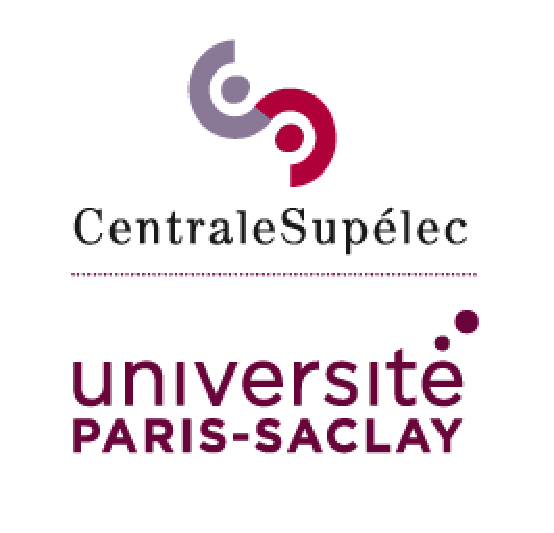
\includegraphics[scale=0.7]{../../../Decision-Modeling/LectureNotes/source/CS-logo}
\par\end{center}

\begin{flushright}
Professor: Tom Dupuis
\par\end{flushright}

\begin{flushright}
Student e-mail: jose-antonio.lorencio-abril@student-cs.fr
\par\end{flushright}

\newpage{}

\lyxaddress{This is a summary of the course \emph{Machine Learning} taught at
the Universit� Paris Saclay - CentraleSup�lec by Professor Tom Dupuis
in the academic year 23/24. Most of the content of this document is
adapted from the course notes by Dupuis, \cite{Dupuis2023}, so I
won't be citing it all the time. Other references will be provided
when used.}

\tableofcontents{}

\newpage{}

\part{Deep Learning}

\section{Introduction}

\textbf{Artificial Intelligence} is a wide concept, encompassing different
aspects and fields. We can understand the term AI as the multidisciplinary
field of study that aims at recreating human intelligence using artificial
means. This is a bit abstract, and, in fact, there is no single definition
for what this means. Intelligence is not fully understood, and thus
it is hard to assess whether an artificial invention has achieved
intelligence, further than intuitively thinking so.

For instance, AI involves a whole variety of fields:
\begin{itemize}
\item Perception
\item Knowledge
\item Cognitive System
\item Planning
\item Robotics
\item Machine Learning (Neural Networks)
\item Natural Language Processing
\end{itemize}
Leveraging all of these, people try to recreate or even surpass human
performance in different tasks. For example, a computer program that
can play chess better than any human could ever possibly play, such
as Stockfish, or a system that is able to understand our messages
and reply, based on the knowledge that it has learnt in the past,
such as ChatGPT and similar tools. Other examples are self-driving
cars, auto-controlled robots, etc.

Therefore, AI is a very wide term, which merges many different scientific
fields. \textbf{Machine Learning}, on the other side, is a narrower
term, which deals with the study of the techniques that we can use
to make a computer learn to perform some task. It takes concepts from
Statistics, Optimization Theory, Computer Science, Algorithms, etc.
A relevant subclass of Machine Learning, which has come to be one
of the most prominent fields of research in the recent years, is \textbf{Neural
Networks }or \textbf{Deep Learning}, which consists on an ML technique
based on the human brain. Many amazing use cases that we see everywhere,
like Siri (Apple assistant), Cortana (Windows assistant), Amazon recommender
system, Dall-E (OpenAI image generation system), etc. Not only this,
but the trend is growing, and the interest in DL is continuously increasing.

This is partly also due to the increase in computing resources, and
the continuous optimization that different techniques are constantly
experiencing. For instance, for a model trained on one trillion data
points, in 2021 the training process required around 16500x less compute
than a model trained in 2012.

But not everything is sweet and roses when using DL. Since these systems
are being involved in decision making processes, there are some questions
that arise, like whose responsibility is it when a model fails? Moreover,
data is needed to train the models, so it is relevant to address how
datasets should be collected, and to respect the privacy of the people
that produce data. In addition, the recent technologies that are able
to generate new content and to modify real content, make it a new
issue that AI can create false information, mistrust, and even violence
or paranoia.

Nonetheless, let's not focus on the negative, there are lots of nice
applications of DL, and it is a key component to deal with data, achieving
higher performance than traditional ML techniques for huge amount
of data.

\subsection{AI History}

In 1950, Alan turing aimed to answer the question '\emph{Can machines
think?}' through a test, which came to be named the \textbf{Turing
Test}, and consists in a 3 players game. First, a similar game is
the following: 2 talkers, a man and a female, and 1 interrogator.
The interrogator asks questions to the talkers, with the aim of determining
who is the man and who is the female. The man tries to trick the interrogator,
while the woman tries to help him to identify her.

Then, the Turing Test consists in replacing the man by an artificial
machine. Turing thought that a machine that could trick a human interrogator,
should be considered intelligent.

Later, in 1956, in the Dartmouth Workshop organized by IBM, the term
\textbf{Artificial Intelligence} was first used to describe \emph{every
aspect of learning or any other feature of intelligence can be so
precisely described that a machine can be made to simulate it}.

From this year on, there was a focus on researching about \textbf{Symbolic
AI}, specially in three areas of research:
\begin{itemize}
\item Reasoning as search: a different set of actions leads to a certain
goal, so we can try to find the best choice of action to obtain the
best possible outcome.
\item Natural Language: different tools were developed, following grammar
and language rules.
\item Micro world: small block based worlds, that the system can identify
and move.
\end{itemize}
In 1958, the \textbf{Perceptron} was conceived, giving birth to what
is called the connectionism, an approach to AI based on the human
brain, and a big hype that encouraged funding to support AI research.
At this era, scientists experience a bit of lack of perspective, thinking
that the power of AI was much higher than it was. For instance, H.
A. Simon stated in 1965 that '\emph{machines will be capable, within
twenty years, of doing any work a man can do.}' We can relate to our
time, with the huge hype that AI is experiencing, as well as the many
apocaliptic theories that some people are making. Maybe we are again
overestimating the power of AI.

The time from 1974 to 1980 is seen as the first winter of AI, in which
research was slowed down and funding was reduced. This was due to
several problems found at the time:
\begin{itemize}
\item There were few computational resources.
\item The models at the time were not scalable.
\item The Moravec's paradox: it is comparatively easy to make computers
exhibit adult level performance on intelligence test or playing checkers,
and difficult or impossible to give them the skills of a one-year-old
when it comes to perception and mobility.
\item Marvin Minsky made some devastating critics to connectionism, compared
to symbolic, rule-based models:
\begin{itemize}
\item Limited capacity: Minsky showed that single-layer perceptrons (a simple
kind of neural network) could not solve certain classes of problems,
like the XOR problem. While it was later shown that multi-layer perceptrons
could solve these problems, Minsky's work resulted in a shift away
from neural networks for a time.
\item Lack of clear symbols: Minsky believed that human cognition operates
at a higher level with symbols and structures (like frames and scripts),
rather than just distributed patterns of activation. He often argued
that connectionist models lacked a clear way to represent these symbolic
structures.
\item Generalization and Abstraction: Minsky was concerned that connectionist
models struggled with generalizing beyond specific training examples
or abstracting high-level concepts from raw data.
\item Inefficiency: Minsky pointed out that many problems which seemed simple
for symbolic models could be extremely computationally intensive for
connectionist models.
\item Lack of explanation: Connectionist models, especially when they become
complex, can be seen as \textquotedbl black boxes\textquotedbl ,
making it difficult to interpret how they arrive at specific conclusions.
\item Over-reliance on learning: Minsky believed that not all knowledge
comes from learning from scratch, and some of it might be innate or
structured in advance. He felt connectionism put too much emphasis
on learning from raw data.
\end{itemize}
\end{itemize}
In 1980, there was a boom in expert knowledge systems that made AI
recover interest. An \textbf{expert system} solves specific tasks
following an ensemble of rules based on knowledge facilitated by experts.
A remarkable use case was the XCON sorting system, developed for the
Digital Equipment Corporation, which helped them save 40M\$ per year.
In addition, connectionism also came again on scene, thanks to the
development of \textbf{backpropagation} applied to neurons, by Geoffrey
Hinton. All these achievement made funding to come back to the field.

Nonetheless, there came a second winter of AI, from 1987 to 1994,
mainly because several companies were disappointed and AI was seen
as a technology that couldn't solve wide varieties of tasks. The funding
was withdrawn from the field and a lot AI companies went bankrupt.

Luckily, from 1995 there started a new return of AI in the industry.
The Moore's Law states that speed and memory of computer doubles every
two years, and so computing power and memory was rapidly increasing,
making the use of AI systems more feasible each year. During this
time, many new concepts were introduced, such as \textbf{intelligent
agents} as systems that perceive their environment and take actions
which maximize their chances of success; or different \textbf{probabilistic
reasoning tools} such as Bayesian networks, hidden Markov models,
information theory, SVM,... In addition, AI researchers started to
reframe their work in terms of mathematics, computer science, physics,
etc., making the field more attractive for funding. A remarkable milestone
during this time was the victory of Deep Blue against Garry Kasparov.

The last era of AI comes from 2011 to today, with the advent and popularization
of \textbf{Deep Learning} (DL), which are deep graph processing layers
mimicking human neurons interactions. This happened thanks to the
advances of hardware technologies, that have enabled the enormous
computing requirements needed for DL. The huge hype comes from the
spectacular results shown by this kind of systems in a huge variety
of tasks, such as computer vision, natural language processing, anomaly
detection,...

In summary, we can see how the history of AI has been a succession
of hype and dissapointment cycles, with many actors involved and the
industry as a very important part of the process.

\section{Machine Learning Basics}

In this section, we review some notation, and basic knowledge of Linear
Algebra, Probability and Machine Learning.

\subsection{Linear Algebra Basics}

A \textbf{scalar} is a number, either real and usually denoted $x\in\mathbb{R}$,
or natural and denoted $n\in\mathbb{N}$. A \textbf{vector} is an
array of numbers, usually real, $x\in\mathbb{R}^{n},$ or
\[
x=\left[\begin{array}{c}
x_{1}\\
x_{2}\\
\vdots\\
x_{n}
\end{array}\right].
\]
 A \textbf{matrix} is a 2-dimensional array of numbers, $A\in\mathbb{R}^{n\times m}$,
or
\[
A=\left[\begin{array}{ccc}
A_{11} & \dots & A_{1n}\\
\vdots & \ddots & \vdots\\
A_{m1} & \dots & A_{mn}
\end{array}\right].
\]
 A \textbf{tensor} is an $n$-dimensional array of numbers, for example
$A\in\mathbb{R}^{m\times k\times p}$ is a 3-dimensional tensor.

Usually, we will be working with matrices, which can be operated in
different ways:
\begin{itemize}
\item Transposition: $A^{T}$ is the transposed of $A$, defined as $\left(A^{T}\right)_{ij}=A_{j,i}$.
\item Multiplication: Let $A\in\mathbb{R}^{m\times k},B\in\mathbb{R}^{k\times n}$,
their multiplication, $C\in\mathbb{R}^{m\times n}$ is defined as
\[
C=A\cdot B=AB=\left(C_{ij}\right)_{i\leq m,j\leq n}=\left(\sum_{k}A_{ik}B_{kj}\right)_{i\leq m,j\leq n}.
\]
 Note that the following holds for every matrix $A,B$:
\[
\left(AB\right)^{T}=B^{T}A^{T}.
\]
\item Point-wise operations: if we have two matrices of the same size, $A,B\in\mathbb{R}^{m\times n}$,
we can use apply scalar operator point-wise to each pair of elements
in the same position in the two matrices. For example, the sum or
the substraction of matrices.
\end{itemize}
There are also special matrices:
\begin{itemize}
\item Identity matrix: the identity matrix is a square matrix that preserves
any vector it is multiplied with. For vectors of size $n$, the identity
matrix $I_{n}$ verifies
\[
I_{n}x=x,\forall x\in\mathbb{R}^{n}.
\]
\item Inverse matrix: the inverse of a square matrix, $A\in\mathbb{R}^{n\times n}$,
when it exists, is defined as the only matrix $A^{-1}$ such that
\[
A^{-1}A=AA^{-1}=I_{n}.
\]
\end{itemize}
Another important concept is that of the norm, which is basically
measuring how far a point is from the origin of the space and can
be used to measure distances:

\begin{tcolorbox}
\begin{defn}
A \textbf{norm} is a function $f$ that measures the size of vectors,
and must have the following properties:
\begin{itemize}
\item $f\left(x\right)=0\iff x=0,$
\item $f\left(x+y\right)\leq f\left(x\right)+f\left(y\right),$ and
\item $\forall\alpha\in\mathbb{R},f\left(\alpha x\right)=\left|\alpha\right|f\left(x\right).$
\end{itemize}
\end{defn}
\end{tcolorbox}

A very important family of norms is the $L^{p}$ norm, defined as
\[
\left\Vert x\right\Vert _{p}=\left(\sum_{i}\left|x_{i}\right|^{p}\right)^{\frac{1}{p}}.
\]
 The \textbf{Euclidean norm} is the $L^{2}$ norm, noted $\left\Vert x\right\Vert $
and equivalent to computing $\sqrt{x^{T}x}$. In Machine Learning,
it is not uncommon to find the use of the squared Euclidean norm,
since it maintains the ordinals and is easier to operate with. The
\textbf{Manhattan norm} is the $L^{1}$ norm, and it is used when
the difference between zero and nonzero elements is important. Finally,
the \textbf{Max norm} is the $L^{\infty}$, or $\left\Vert x\right\Vert _{\infty}=\max_{i}\left|x_{i}\right|$.

\subsection{Probability Basics}

A \textbf{random variable}, $X$, is a variable that can take different
values, $x$, randomly. They can be \textbf{discrete}, like the number
drawn from a dice, or \textbf{continuous}, like the humidity in the
air.

A probability distribution, $p$, is a \textbf{Probability Mass Function
(PMF)} for discrete variables, and a \textbf{Probability Density Function
(PDF)} for continuous random variables. It must satisfy:
\begin{itemize}
\item The domain of $p$ describe all possible states of $X$.
\item $\forall x\in X,p\left(x\right)\geq0$.
\item $\int_{x\in X}p\left(x\right)dx=1$.
\end{itemize}
It is usual to have two (or more) random variables, $X$ and $Y$,
and to be interested in the probability distribution of their combination,
$p\left(x,y\right)$. In this context, we define the \textbf{marginal
probability} of the variable $X$ as
\[
p\left(X=x\right)=\int_{y\in Y}p\left(x,y\right)dy,\forall x\in X.
\]
 The \textbf{conditional probability} of the variable $Y$ conditioned
to $X=x$ is
\[
p\left(Y=y|X=x\right)=\frac{p\left(Y=y,X=x\right)}{P\left(X=x\right)}.
\]
 Finally, there is the \textbf{chain rule of conditional probabilities},
in which we start with $n$ random variables, $X_{1},...,X_{n}$,
and it follows:
\[
p\left(X_{1}=x_{1},...,X_{n}=x_{n}\right)=p\left(X_{1}=x_{1}\right)\prod_{i=2}^{n}p\left(X_{i}=x_{i}|X_{1}=x_{1},...,X_{i-1}=x_{i-1}\right).
\]

\begin{example}
For example, let's say $X=\left\{ 1,2,3\right\} $, $Y=\left\{ 1,2\right\} $
and $Z=\left\{ 1,2\right\} $ with the following probabilities:
\begin{center}
\begin{tabular}{|c|c|c|c|}
\hline 
$X$ & $Y$ & $Z$ & $p\left(x,y,z\right)$\tabularnewline
\hline 
\hline 
1 & 1 & 1 & $\frac{1}{6}$\tabularnewline
\hline 
1 & 1 & 2 & $\frac{1}{6}$\tabularnewline
\hline 
1 & 2 & 1 & $\frac{1}{12}$\tabularnewline
\hline 
1 & 2 & 2 & $\frac{1}{24}$\tabularnewline
\hline 
2 & 1 & 1 & $\frac{1}{24}$\tabularnewline
\hline 
2 & 1 & 2 & $\frac{1}{20}$\tabularnewline
\hline 
2 & 2 & 1 & $\frac{1}{20}$\tabularnewline
\hline 
2 & 2 & 2 & $\frac{1}{20}$\tabularnewline
\hline 
3 & 1 & 1 & $\frac{1}{6}$\tabularnewline
\hline 
3 & 1 & 2 & $\frac{1}{12}$\tabularnewline
\hline 
3 & 2 & 1 & $\frac{1}{20}$\tabularnewline
\hline 
3 & 2 & 2 & $\frac{1}{20}$\tabularnewline
\hline 
\end{tabular}
\par\end{center}

Then, the marginal probabilities for the variable $X$ are
\[
P\left(X=1\right)=\frac{1}{6}+\frac{1}{6}+\frac{1}{12}+\frac{1}{24}=\frac{11}{24},
\]
\[
P\left(X=2\right)=\frac{1}{24}+\frac{1}{20}+\frac{1}{20}+\frac{1}{20}=\frac{23}{120},
\]
\[
P\left(X=3\right)=\frac{1}{6}+\frac{1}{12}+\frac{1}{20}+\frac{1}{20}=\frac{21}{60}=\frac{7}{20}.
\]

The conditional probability for the event $\left\{ Y=1|X=3\right\} $
is:
\[
P\left(Y=1|X=3\right)=\frac{P\left(Y=1,X=3\right)}{P\left(X=3\right)}=\frac{\frac{1}{6}+\frac{1}{12}}{\frac{7}{20}}=\frac{\frac{1}{4}}{\frac{7}{20}}=\frac{5}{7}.
\]

The conditional probability for the event $\left\{ Z=1|X=3,Y=1\right\} $
is:
\[
P\left(Z=1|X=3,Y=1\right)=\frac{P\left(X=3,Y=1,Z=1\right)}{P\left(X=3,Y=1\right)}=\frac{\frac{1}{6}}{\frac{1}{4}}=\frac{2}{3}.
\]

The probability of the event $\left\{ X=3,Y=1,Z=1\right\} $ could
be computed from the conditional probabilities as follows, in case
we only knew these:
\begin{align*}
P\left(X=3,Y=1,Z=1\right)= & P\left(X=3\right)\cdot P\left(Y=1|X=3\right)\cdot P\left(Z=1|X=3,Y=1\right)\\
= & \frac{7}{20}\cdot\frac{5}{7}\cdot\frac{2}{3}=\frac{10}{60}=\frac{1}{6}.
\end{align*}
\end{example}
When there are several variables, it is possible that the value of
one of them is dependant, somehow, on the values that the other variables
take; or that it is not:

\begin{tcolorbox}
\begin{defn}
Two random variables $X$ and $Y$ are \textbf{independant}, denoted
$X\perp Y$, if $\forall x\in X,y\in Y,p\left(X=x,Y=y\right)=p\left(X=x\right)\cdot p\left(Y=y\right).$ 

$X$ and $Y$ are \textbf{conditionally independent} given the random
variable $Z$, written $X\perp_{Z}Y$ if $\forall x\in X,y\in Y,z\in Z$,
\[
p\left(X=x,Y=y|Z=z\right)=p\left(X=x|Z=z\right)\cdot p\left(Y=y|Z=z\right).
\]
\end{defn}
\end{tcolorbox}

In Statistics and Machine Learning, there are some measures that summarize
information about random variables, and that hold great importance.

\begin{tcolorbox}
\begin{defn}
The \textbf{expectation} of a function $f\left(x\right)$ where $x\sim p\left(x\right)$
is the average value of $f$ over $x$:
\[
\mathbb{E}_{x\sim p}\left[f\left(x\right)\right]=\int_{x\in X}p\left(x\right)f\left(x\right)dx.
\]
 The \textbf{variance} of $f\left(x\right)$ measures how the values
of $f$ varies from its average:
\[
Var\left[f\left(x\right)\right]=\mathbb{E}\left[\left(f\left(x\right)-\mathbb{E}\left[f\left(x\right)\right]\right)^{2}\right],
\]
 and the \textbf{standard deviation }is the square root of the variance.

The \textbf{covariance} of two random variables provides informaiton
about how much two values are linearly related. More generally, if
we apply two functions $f\left(x\right),$ where $x\sim p\left(x\right)$,
and $g\left(y\right)$, where $y\sim p\left(y\right)$, the covariance
between them is:
\[
Cov\left[f\left(x\right),g\left(y\right)\right]=\mathbb{E}\left[\left(f\left(x\right)-\mathbb{E}\left[f\left(x\right)\right]\right)\left(g\left(y\right)-\mathbb{E}\left[g\left(y\right)\right]\right)\right].
\]
\end{defn}
\end{tcolorbox}


\subsection{Machine Learning Basics}

To finalize with this review chapter, we are going to remember some
basic concepts of Machine Learning.

First, let's give a definition of the concept:

\begin{tcolorbox}
\begin{defn}
A computer program is said to \textbf{learn} from experience $E$
with respect to some class of tasks $T$ and performance measure $P$,
if its performance at tasks in $T$, as measured by $P$, improves
with experience $E$.
\end{defn}
\end{tcolorbox}

\begin{itemize}
\item The \textbf{task} $T$ can be classification, regression, translation,
generation, anomaly detection,...
\item The \textbf{performance measure $P$ }is specific to the tasks involved,
and can be accuracy for classification, for example. It is measured
on a \textbf{test set}.
\item The \textbf{experience} $E$ is divided into two main categories:
\begin{itemize}
\item \textbf{Supervised learning}: a dataset of points associated with
a label or a target determines the expected outcome of each event.
\item \textbf{Unsupervised learning}: a dataset of points without labels
or targets, in which the desirable outcome needs to be define in some
different way.
\end{itemize}
\end{itemize}
Mathematically, we can formalize this as having a dataset of $m$
points and $k$ features, which can be represented as a matrix $X\in\mathbb{R}^{m\times k}$.
In the case of supervised learning, $X$ is associated with a vector
of labels, $y$, and we aim to learn a joint distribution, $p\left(X,y\right)$
to infer
\[
p\left(Y=y|X=x\right)=\frac{p\left(x,y\right)}{\sum_{y'}p\left(x,y'\right)}.
\]
 The goal is then to find a function $\hat{f}$ that associates each
$x$ to the best approximation of $y$, and that is capable of generalizing
to unseen data. Usually, $\hat{f}$ is parameterized by a set of parameters,
$\theta$, which are learnt during training.

The main challenge of an ML model is \textbf{generalization} to unseen
data estimated on test data after the training on training data. \textbf{Overfitting}
occurs when the gap between training error and test error is too large,
while \textbf{underfitting} occurs when the training error is too
large. The \textbf{capacity} of a model is the range of functions
that it is able to leanr and control how likely the model can overfit
or underfit. This is visualized in Figure \ref{fig:Appropriate-capacity,-overfittin}.

\begin{figure}
\begin{centering}
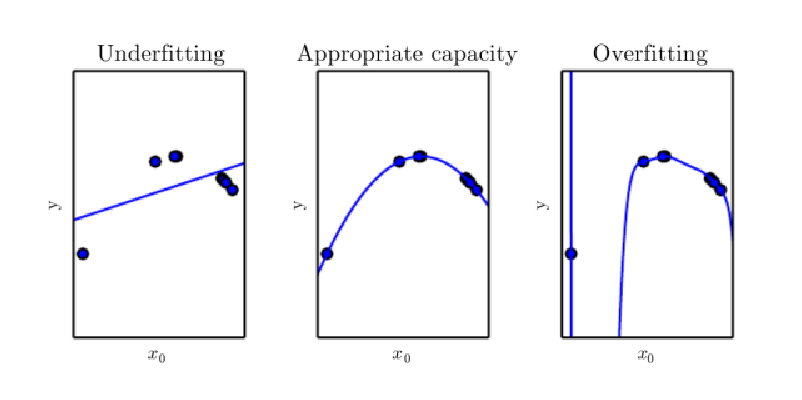
\includegraphics[scale=0.7]{pegado1}
\par\end{centering}
\caption{\label{fig:Appropriate-capacity,-overfittin}Appropriate capacity,
overfitting and underfitting visualization.}
\end{figure}

When we want to train a model, we will define the parameters that
characterize it, and then we need to obtain the best possible of the
parameters, according to the data. For this, we use estimators:

\begin{tcolorbox}
\begin{defn}
Given an unknown parameter $\theta$, we estimate it through an \textbf{estimator},
$\hat{\theta}$. A \textbf{point estimator} is a function of the data,
$X$,
\[
\hat{\theta}=g\left(X\right).
\]
 The \textbf{bias} of an estimator is
\[
bias\left(\hat{\theta}\right)=\mathbb{E}\left[\hat{\theta}\right]-\theta.
\]
 An estimator is \textbf{unbiased }if $bias\left(\hat{\theta}\right)=0$.

The \textbf{variance} of an estimator is $Var\left(\hat{\theta}\right)$.
\end{defn}
\end{tcolorbox}

There are different ways to construct estimators, but one that is
frequently used and that has solid mathematical foundations is the
\textbf{maximum likelihood estimator}. Consider a dataset $X=\left\{ x_{1},...,x_{n}\right\} $
and $p\left(x;\theta\right)$ a parametric family of probability distribution
that maps for each $x$ the probability $p_{data}\left(x\right)$.
This is, for each $\theta$, $p\left(x;\theta\right)$ is a probability
density function. The maximum likelihood estimator is then
\begin{align*}
\theta_{ML}= & \arg\max_{\theta}p_{model}\left(X;\theta\right)\\
= & \arg\max_{\theta}\prod_{i=1}^{n}p_{model}\left(x_{i};\theta\right),
\end{align*}
 considering that all instances of data are independent and identically
distributed (iid). It is also a common practice to use the maximum
\textbf{log}-likelihood instead, removing the product and avoiding
floating point issues, since when the dataset is large, the product
will rapidly go to 0. In addition, the logarithm does not modify the
ordinals of the function. Therefore, we can use:
\[
\theta_{ML}=\arg\max_{\theta}\sum_{i=1}^{n}\log\left(p_{model}\left(x_{i};\theta\right)\right).
\]


\section{Deep Neural Networks}

\subsection{Perceptron}

A deeper explanation of the perceptron can be read in my notes from
another course, \url{https://lorenc1o.github.io/BDMA_Notes/universities/UPC/Machine_Learning_summary.pdf}.

A perceptron is an algorithm for supervised learning of binary classifiers.
That is, we have a dataset $X\in\mathbb{R}^{n\times m}$ associated
with a vector of labels $y\in\left\{ 0,1\right\} ^{n}$. Then, the
perceptron learns a function $\hat{f}$ parametrized by a vector of
weights $w\in\mathbb{R}^{m}$ and a bias $b$, such that:
\[
\hat{f}\left(x\right)=\begin{cases}
1 & if\ w\cdot x+b>0\\
0 & \sim
\end{cases}.
\]

Therefore, it is a linear classifier, which divides the input space
into two regions separated by a hyperplane. This means that a perceptron
cannot separate non-linear data.

\subsection{Multi-layer perceptron}

A deeper explanation of the MLP can be read in my notes from another
course, \url{https://lorenc1o.github.io/BDMA_Notes/universities/UPC/Machine_Learning_summary.pdf}.

When we say 'Deep' neural network, we refer to a series of stacked
perceptrons. However, just like this, the model is still linear. This
is why activation functions are introduced. An \textbf{activation
function} is a function that is applied to the output of a perceptron,
to make it non linear.

For example, ReLU is a piecewise-linear function defined as
\[
ReLU\left(z\right)=\begin{cases}
z & if\ z\geq0\\
0 & \sim
\end{cases}=\max\left\{ z,0\right\} .
\]
 This function preserves much of the good oprimization properties
of a linear function, i.e., it is differentiable (apart from one point),
and its derivative is constant.
\begin{example}
Learn the XOR function with a 2-layer MLP.

The XOR function is represented with the table:
\begin{center}
\begin{tabular}{|c|c|c|}
\hline 
$x_{1}$ & $x_{2}$ & $y$\tabularnewline
\hline 
\hline 
0 & 0 & 0\tabularnewline
\hline 
0 & 1 & 1\tabularnewline
\hline 
1 & 0 & 1\tabularnewline
\hline 
1 & 1 & 0\tabularnewline
\hline 
\end{tabular}
\par\end{center}

We want to use a 2-layer MLP to learn this function:
\begin{center}
\includegraphics[scale=0.6]{xor\lyxdot drawio}
\par\end{center}

In $h_{1}$, it will be
\[
w_{11}x_{1}+w_{12}x_{2}+b_{1},
\]
 and in $h_{2}$
\[
w_{11}x_{1}+w_{12}x_{2}+b_{1}.
\]
 This can be represented as
\[
h=W_{h}^{T}X+b_{h}.
\]
 Then, we apply ReLU
\[
\max\left(0,W_{h}^{T}X+b_{h}\right),
\]
 and finally the output layer
\[
y=W_{y}^{T}\max\left(0,W_{h}^{T}X+b_{h}\right)+b_{y}.
\]

Let's see the different inputs:
\begin{center}
\begin{tabular}{|c|c|c|c|}
\hline 
$x_{1}$ & $x_{2}$ & $h$ & $y$\tabularnewline
\hline 
\hline 
0 & 0 & $\left(\begin{array}{cc}
w_{11} & w_{12}\\
w_{21} & w_{22}
\end{array}\right)\left(\begin{array}{c}
0\\
0
\end{array}\right)+\left(\begin{array}{c}
b_{1}\\
b_{2}
\end{array}\right)=\left(\begin{array}{c}
b_{1}\\
b_{2}
\end{array}\right)$ & $\left(\begin{array}{cc}
w_{1}^{y} & w_{2}^{y}\end{array}\right)\left(\begin{array}{c}
\max\left(0,b_{1}\right)\\
\max\left(0,b_{2}\right)
\end{array}\right)+b_{y}\leq0$\tabularnewline
\hline 
0 & 1 & $\left(\begin{array}{c}
w_{12}+b_{1}\\
w_{22}+b_{2}
\end{array}\right)$ & $\left(\begin{array}{cc}
w_{1}^{y} & w_{2}^{y}\end{array}\right)\left(\begin{array}{c}
\max\left(0,w_{12}+b_{1}\right)\\
\max\left(0,w_{22}+b_{2}\right)
\end{array}\right)+b_{y}>0$\tabularnewline
\hline 
1 & 0 & $\left(\begin{array}{c}
w_{11}+b_{1}\\
w_{21}+b_{2}
\end{array}\right)$ & $\left(\begin{array}{cc}
w_{1}^{y} & w_{2}^{y}\end{array}\right)\left(\begin{array}{c}
\max\left(0,w_{11}+b_{1}\right)\\
\max\left(0,w_{21}+b_{2}\right)
\end{array}\right)+b_{y}>0$\tabularnewline
\hline 
1 & 1 & $\left(\begin{array}{c}
w_{11}+w_{12}+b_{1}\\
w_{21}+w_{22}+b_{2}
\end{array}\right)$ & $\left(\begin{array}{cc}
w_{1}^{y} & w_{2}^{y}\end{array}\right)\left(\begin{array}{c}
\max\left(0,w_{11}+w_{12}+b_{1}\right)\\
\max\left(0,w_{21}+w_{22}+b_{2}\right)
\end{array}\right)+b_{y}\leq0$\tabularnewline
\hline 
\end{tabular}
\par\end{center}

A solution is:
\[
W_{h}=\left(\begin{array}{cc}
1 & 1\\
1 & 1
\end{array}\right),b_{h}=\left(\begin{array}{c}
0\\
-1
\end{array}\right),W_{y}=\left(\begin{array}{c}
1\\
-2
\end{array}\right),b=0.
\]
 Let's check:
\begin{center}
\begin{tabular}{|c|c|c|c|}
\hline 
$x_{1}$ & $x_{2}$ & $h$ & $y$\tabularnewline
\hline 
\hline 
0 & 0 & $\left(\begin{array}{c}
0\\
-1
\end{array}\right)$ & $\left(\begin{array}{cc}
1 & -2\end{array}\right)\left(\begin{array}{c}
0\\
0
\end{array}\right)=0\leq0$\tabularnewline
\hline 
0 & 1 & $\left(\begin{array}{c}
1\\
1-1
\end{array}\right)$ & $\left(\begin{array}{cc}
1 & -2\end{array}\right)\left(\begin{array}{c}
1\\
0
\end{array}\right)=1>0$\tabularnewline
\hline 
1 & 0 & $\left(\begin{array}{c}
1\\
1-1
\end{array}\right)$ & $\left(\begin{array}{cc}
1 & -2\end{array}\right)\left(\begin{array}{c}
1\\
0
\end{array}\right)=1>0$\tabularnewline
\hline 
1 & 1 & $\left(\begin{array}{c}
1+1\\
1+1-1
\end{array}\right)$ & $\left(\begin{array}{cc}
1 & -2\end{array}\right)\left(\begin{array}{c}
2\\
1
\end{array}\right)=0\leq0$\tabularnewline
\hline 
\end{tabular}
\par\end{center}

So, it works! Note that this solution is not unique!

What happens is actually that the solution for the XOR problem is
not linearly separable:
\begin{center}
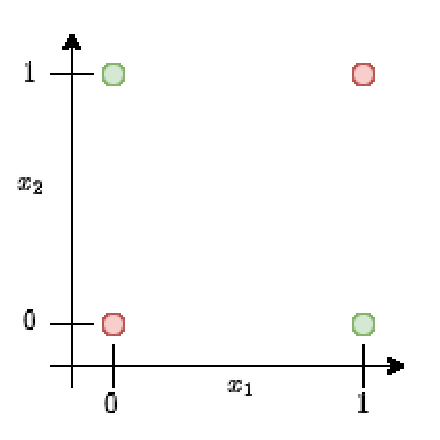
\includegraphics[scale=0.6]{xor_space}
\par\end{center}

But, the hidden layer transforms this space, making the problem linearly
separable, and therefore solvable in the last layer:
\begin{center}
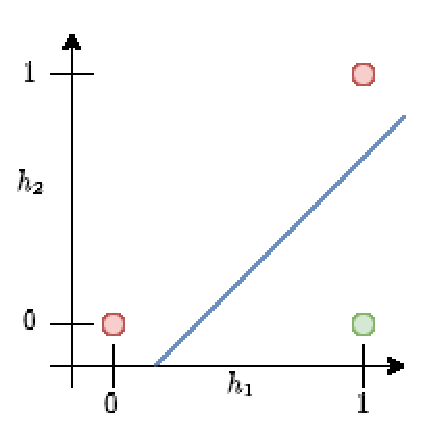
\includegraphics[scale=0.6]{xor_space_trans}
\par\end{center}
\end{example}

\subsection{Cost Functions}

The cost function is important when working with neural networks,
because our goal is to ultimately train the model to solve some problem,
and the cost functions will be the function that our model will aim
at minimizing, thus guiding the training process.

Usually, we will need to choose a cost function $\mathcal{L}$ that
is suitable for our problem. Then, we will minimize $\mathcal{L}$
with stochastic gradient descent, by:
\begin{itemize}
\item Training on a training dataset.
\item Estimating error on an evaluation dataset.
\item Computing the gradients using backpropagation.
\end{itemize}
In this process, we will aim to find good local minima, instead of
global minimum. This is related to overfitting (learning only the
training data, losing generalization capabilities), and to the empirical
fact that deep neural network have surprisingly good local and non-global
optima.

\subsubsection{Choice of cost function}

In the general case, we use the maximum likelihood principle, taking
the output types of the network into account. This means that we assume
our dataset $\left\{ x_{1},...,x_{n}\right\} $ to be independently
and identically distributed (i.i.d.) from an unknown distribution,
$p_{data}\left(x\right)$. We choose a parametric model family $p_{model}\left(x;\theta\right)$
represented as a neural network, which we use to estimate an approximation
of the true distribution. For this, we utilize the \textbf{maximum
likelihood estimator}, defined as
\[
\theta_{ML}=\arg\max_{\theta}\prod_{i=1}^{n}p_{model}\left(x_{i};\theta\right).
\]
 Usually, to avoid floating point errors, the log-likelihood is used
instead:
\[
\theta_{ML}=\arg\max_{\theta}\sum_{i=1}^{n}\log p_{model}\left(x_{i};\theta\right).
\]

In the maximum likelihood estimation framework, we might apply activation
functions to the output layer to get a desired structure for our distribution.
This choice will also influence the mathematical form of the cost
function. For example, we can use linear units for regression or for
Gaussian distributions, sigmoid units for binary classification or
softmax units for multi-class classification.

\paragraph{Linear units for regression}

A \textbf{linear output layer} is such that, given the features $h$,
the output is
\[
\hat{y}=W^{T}h+b,
\]
 where $W$ is the weights vector and $b$ the bias.

We can use this to predict real or vector valued variables, such as
prices, biometrics,...

\paragraph{Linear unit for Gaussian distribution}

A \textbf{Gaussian output unit} is such that, given features $h$,
a linear layer produces a vector $\hat{y}$ representing the mean
and the covariance matrix of a conditional Gaussian distribution:
\[
p\left(y|x\right)=\mathcal{N}\left(y;\hat{y},I\right).
\]

Covariance is usually not modelled or simplified to be diagonal (in
which case we need to ensure that the output is non-negative).

\paragraph{Binary classification}

In this case, the objective is to predict a binary variable, $y$:
the neural network must predict $P\left(y=1|x\right)$. Thus, we must
ensure that the output is a probability, in the interval $\left[0,1\right]$.
For this, we can take
\[
P\left(y=1|x\right)=\max\left\{ 0,\min\left\{ 1,W^{T}h+b\right\} \right\} .
\]
 The problem with this approach is that if $W^{T}h+b\notin\left[0,1\right]$
then the gradient is 0 and the training will stop. To solve this issue,
we can use a \textbf{sigmoid unit}, which is 
\[
\hat{y}=\sigma\left(W^{T}h+b\right)=\frac{1}{1+e^{-W^{T}h+b}}.
\]


\paragraph{Softmax unit for multi-class classification}

Now our objective is to classify the input data into one among $N>2$
classes. We want to predict $\hat{y}$ with $\hat{y_{i}}P\left(y=i|x\right)$,
subject to $\hat{y_{i}}\in\left[0,1\right],\forall i$ and $\sum_{i}y_{i}=1$.

In the output layer we can have $N$ perceptrons, each of them computing
$z_{i}=\log P\left(y=i|x\right)$, i.e., the \textbf{logits}. With
this, we can apply the \textbf{softmax output unit} to all of them,
obtaining our vector of probabilities, as
\[
softmax\left(z\right)_{i}=\frac{e^{z_{i}}}{\sum_{j}e^{z_{j}}}.
\]


\subsubsection{Cross-entropy}

In classification problems we want to estimate the probability of
different outcomes. Let the estimated probability of outcome $i$
be $p_{model}\left(x=i\right)$ with to-be-optimized parameters $\theta$
and let the frequency of outcome $i$ in the training set be $p\left(x=i\right)$.
Given $N$ conditionally independent samples in the training set,
then the likelihood of the parameters $\theta$ of the model $p_{model}\left(x=i\right)$
on the training set is:
\[
\mathcal{L}\left(\theta\right)=\prod_{i\in X}p_{model}\left(x=i\right)^{N\cdot p\left(x=i\right)}.
\]
 Therefore, the log-likelihood, divided by $N$, is
\[
\frac{1}{N}\log\left(\mathcal{L}\left(\theta\right)\right)=\frac{1}{N}N\cdot\sum_{i\in X}p\left(x=i\right)\log p_{model}\left(x=i\right)=\sum_{i\in X}p\left(x=i\right)\log p_{model}\left(x=i\right).
\]

Cross-entropy minimization is frequently used in optimization and
rare-event probability estimation. When comparing a distribution $q$
against a fixed reference distribution $p$, cross-entropy and KL
divergence are identical up to an additive constant (since $p$ is
fixed): According to the Gibbs' inequality, both take on their minimal
values when $p=q$, which is $0$ for KL divergence, and $H\left(p\right)$
for cross-entropy. In the engineering literature, the principle of
minimizing KL divergence (Kullback's \textquotedbl Principle of Minimum
Discrimination Information\textquotedbl ) is often called the Principle
of Minimum Cross-Entropy (MCE), or Minxent.

\subsection{Why deep NN?}

Depth is the longest data path data can take from input to output.
For a deep feed forward NN, depth is the number of hidden layers plus
the output layer. State-of-the-art architectures used in practice
have dozens to hundreds of layers.

\begin{tcolorbox}
\begin{thm}
Universal Approximation Theorem

Let $\varphi\left(\right)$ be a nonconstant, bounded, and monotonically
increasing continuous function. Let $I_{m_{0}}$ denote the $m_{0}-$dimensional
unit hypercube, $\left[0,1\right]^{m_{0}}$. The space of continuous
functions on $I_{m_{0}}$ is denoted by $C\left(I_{m_{0}}\right)$.

Then, given any function $f\in C\left(I_{m_{0}}\right)$ and $\varepsilon>0$,
there exists an integer $m_{1}$ and sets of real constants $\alpha_{i},b_{i}$
and $w_{ij}\in\mathbb{R}$ where $i=1,...,m_{1}$ and $j=1,...,m_{0}$
such that we may define
\[
F\left(x\right)=\sum_{i=1}^{m_{1}}\alpha_{i}\cdot\varphi\left(\sum_{j=1}^{m_{0}}w_{ij}\cdot x_{j}+b_{i}\right)
\]
 as an approximate realization of the function $f$, that is
\[
\left|F\left(x\right)-f\left(x\right)\right|<\varepsilon,\forall x\in I_{m}.
\]
\end{thm}
\end{tcolorbox}

This theorem is very relevant, because it says that for any mapping
function $f$ in supervised learning, there exists a MLP with $m_{1}$
neurons in the hidden layer which is able to approximate it with a
desired precision.

However, it only proves the existence of a shallow (just one hidden
layer) MLP with $m_{1}$ neurons in the hidden layer that can approximate
the function, but it does not tell how to find this number.

As a rule of thumb for the generalization error, it is
\[
\varepsilon=\frac{VC_{dim}\left(MLP\right)}{N},
\]
 where $VC_{dim}$ is the Vapnik-Chervonenkis dimension, a measure
of the capacity of a model. It refers to the largest set of points
that the model can shatter. It is not easy to compute, but a rough
upper bound for a FFNN is $O\left(W\log W\right)$, with $W$ being
the total number of weight in the network.

Also, this theorem hints us that having more neurons in the hidden
layers will give us better training error, but worse generalization
error: overfitting.

However, for most functions $m_{1}$ is very high, and becomes quickly
computationally intractable: so we need to go deeper.

\begin{tcolorbox}
\begin{thm}
No Free Lunch Theorem

Multiple informal formulations:
\begin{itemize}
\item For every learning algorithm A and B, there are as many problems where
A has a better generalization error than problems where B has a better
one.
\item All learning algorithms ahve the same generalization error if we average
over all learning problems.
\item There is no universally better learning algorithm.
\end{itemize}
\end{thm}
\end{tcolorbox}

\begin{tcolorbox}
\textbf{Depth Property}

The number of polygonal regions generated by a MLP with a ReLU function,
$d$ inputs, $n$ neurons per hidden layer and $l$ layers is
\[
O\left(\binom{n}{d}^{d\left(l-1\right)}n^{d}\right).
\]
\end{tcolorbox}

This number grows exponentially with depth. This means that adding
depth basically allows for more transformations of the input space.

\subsection{Gradient-based Learning}

The \textbf{gradient} of a function $f:\mathbb{R}^{n}\rightarrow\mathbb{R}$,
is $\nabla f:\mathbb{R}^{n}\rightarrow\mathbb{R}^{n}$, defined at
the point $p=\left(x_{1},...,x_{n}\right)$ as
\[
\nabla f\left(p\right)=\left(\begin{array}{c}
\frac{\partial f}{\partial x_{1}}\left(p\right)\\
\vdots\\
\frac{\partial f}{\partial x_{n}}\left(p\right)
\end{array}\right).
\]
 This is, it's the local derivative or slope of each dimension at
a certain point.

Going in the opposite direction of the gradient is a na�ve but practical
guess of the direction of the local minimum. This is the base for
the gradient descent method.

\begin{tcolorbox}
\textbf{Gradient-descent method }(Cauchy, 1847)

A parametric function $f\left(\theta\right)$ can be iteratively minimized
by following the opposite direction of the gradient:
\[
\theta_{t+1}=\theta_{t}-\varepsilon\nabla_{\theta}f\left(\theta\right),
\]
 where $\varepsilon>0$ is the \textbf{learning rate}.

We stop iterating when the gradient is near to 0.
\end{tcolorbox}

Notice that this is useless if we have a close form for the gradient!
In that case it is easier to just minimize it. This is useful when
this is not the case, which always happens for neural networks.

In addition, there are variations to the method, for example, we can
vary $\varepsilon$ during training.

\begin{tcolorbox}
\textbf{Stochastic gradient descent}

Given a cost function $f\left(\theta\right)$, parameters of the network
are updated with
\[
\theta\leftarrow\theta-\varepsilon\nabla_{\theta}f\left(\theta\right).
\]

For the negative log-likelihood (MLE), the function is:
\[
f\left(\theta\right)=\frac{1}{m}\sum_{i=1}^{m}L\left(x^{\left(i\right)},y^{\left(i\right)},\theta\right),
\]
 so the estimated gradient is
\[
\nabla_{\theta}f\left(\theta\right)=\frac{1}{m}\sum_{i=1}^{m}\nabla_{\theta}L\left(x^{\left(i\right)},y^{\left(i\right)},\theta\right).
\]
\end{tcolorbox}

The \textcolor{red}{problem} with this approach is that to take a
single step of gradient descent, we must compute the loss over the
whole dataset everytime, making the method not scalable at all. This
is called \textbf{batch gradient descent}.

One \textcolor{lime}{solution} is to compute the gradient with 1 sample
only at each step, which is very noisy and inefficient, but works.
This is the \textbf{stochastic gradient descent}.

In the middle ground, we find the \textbf{mini-batch gradient descent},
which divides the dataset into subsets, and updates the parameters
after processing each of these subsets. A batch is a collection is
a collection of samples used at each iteration for performing SDG
in DL. A bigger batch provides a better gradient estimation, and therefore
a faster learning, but also implies more device memory and slower
descent.

Therefore, there is a tradeoff between money and performance at companies.
In practice, a batch is set between 1 to 256 on one GPU.

But there is an even \textbf{\textcolor{red}{greater problem}}, the
computation of the gradient is computationally very costly. To go
around this problem, \textbf{back-propagation} was invented, as an
efficient technique for gradient computation. 

\subsubsection{Back-propagation}

The back-propagation algorithm is based on the chain rule for the
derivative of composite functions: if we have $y=g\left(x\right)$
and $z=f\left(y\right)=f\left(g\left(x\right)\right)=\left(f\circ g\right)\left(x\right)$,
then
\[
\frac{df}{dx}\left(x\right)=f'\left(g\left(x\right)\right)g'\left(x\right),
\]
 or, abusing notation, 
\[
\frac{dz}{dx}=\frac{dz}{dy}\frac{dy}{dx}.
\]
 This is generalized to multivariate funtions as follows: let $x\in\mathbb{R}^{m},y\in\mathbb{R}^{n},g:\mathbb{R}^{m}\rightarrow\mathbb{R}^{n}$
and $f:\mathbb{R}^{n}\rightarrow\mathbb{R}$. If $z=f\left(y\right)=f\left(g\left(x\right)\right)$,
then
\[
\frac{\partial z}{\partial x_{i}}\left(x\right)=\sum_{j}\frac{\partial z}{\partial y_{j}}\frac{\partial y_{j}}{\partial x_{i}},
\]
 or, 
\[
\nabla_{x}z=\left(\frac{\partial y}{\partial x}\right)^{T}\nabla_{y}z,
\]
 where $\left(\frac{\partial y}{\partial x}\right)$ is the Jacobian
of $g$.

Now, back-propagation is a recursive application of the chain rule,
starting from the cost function. The algorithm works as follows:
\begin{enumerate}
\item \textbf{Forward pass}: a feedforward network takes as input $x$ and
produces the output $\hat{y}$. The information flows from layer to
layer.
\item \textbf{Cost function}: compute the error between expected output
and actual output.
\item \textbf{Back-propagate}: evaluate the individual gradient of each
parameter and propagates them backwards to update them. For this,
we use the concept of \textbf{local derivative}: the derivative of
connected nodes are computed locally on the edges of the graph. For
non-connected nodes, we multiply the edges connected between the nodes,
and we sum over all incoming edges.
\end{enumerate}
If we do this in a forward way, summing over all paths becomes intractable
pretty quickly, while when doing it in a backwards way, it allows
to obtain the derivative of the output with respect to every node
directly in one pass. This leads to massive parallelization.

I did a more detailed explanation, with visualizations in my previous
notes, \url{https://lorenc1o.github.io/BDMA_Notes/universities/UPC/Machine_Learning_summary.pdf}.

\section{Deep Neural Networks: Optimization and Regularization}

\subsection{Optimization}

Recall that neural networks learn by optimizing a cost function, $J\left(\theta\right)$.
This optimization is, in practice, performed by gradient descent,
so we must be able to compute $\nabla_{\theta}J\left(\theta\right)$.
The \textcolor{red}{problem} is that this is computationally very
costly. However, we have seen how back-propagation is an efficient
gradient computation technique.

Now, learning is related to what we want to optimize, since we are
interested in the performance on the test set, which is not always
possible to ensure. Therefore, what is done is minimizing a cost function,
$J$, hoping that it will improve the performance in the test set.
But this relationship is also what makes learning and optimizing two
different things! In pure optimization, our objective is minimizing
$J$, while in learning, the objective is the ability to \textbf{generalize},
or perform well on the test set. Optimizing $J$ on the training set
does not ensure a good generalization, and sometimes worse results
regarding the pure optimization problem in the training set, can yield
better results in the learning problem (think about the overfitting
problem).

Therefore, optimization is a crucial part of learning, and gradient-descent
is a ``cheap'' optimization technique. However, it is not exempt
of problems:
\begin{itemize}
\item Local minima and saddle points: small gradients can stop or greatly
slow down the method.
\item Partial estimation of gradients slows down descent, but can be beneficial
for generalization. This refers to computing the gradient in batches,
instead of in the full dataset (as we saw).
\end{itemize}
In addition, there are problems that are specific to the kind of functions
that arise when working with neural networks:
\begin{itemize}
\item Bad convergence: due to the existence of many local optima.
\item Long training time: the speed of stochastic gradient descent depends
on initialization.
\item Overfitting: deep neural networks have a lot of free parameters. They
can sometimes learn by heart the whole training set, losing the ability
to generalize.
\item Vanishing gradients: in the backpropagation scheme, the first layers
of the network may not receive sufficiently large gradients early
in training.
\end{itemize}
There are different techniques to address these problems. Let's see
some of them.

\subsubsection{Solving Bad Convergence}

It's important to stabilize and improve the convergence of gradient
descent on DNNs, and for this we need good optimization techniques.

\paragraph{Gradient Clipping}

Gradient Clipping proposes to clip the gradient norm to a threshold
$v$, so:
\begin{enumerate}
\item Compute the gradient, say $g$.
\item If $\left\Vert g\right\Vert >th$, then 
\[
g\leftarrow\frac{g\cdot th}{\left\Vert g\right\Vert },
\]
 where $th$ is a threshold to the maximum admissible gradient norm.
\end{enumerate}
This way, we keep the direction of the gradient, while preventing
\emph{overshooting}, i.e., taking too large steps. Although this introduces
a bias in the optimization process, it works well in practice.

A visualization is the following:
\begin{center}
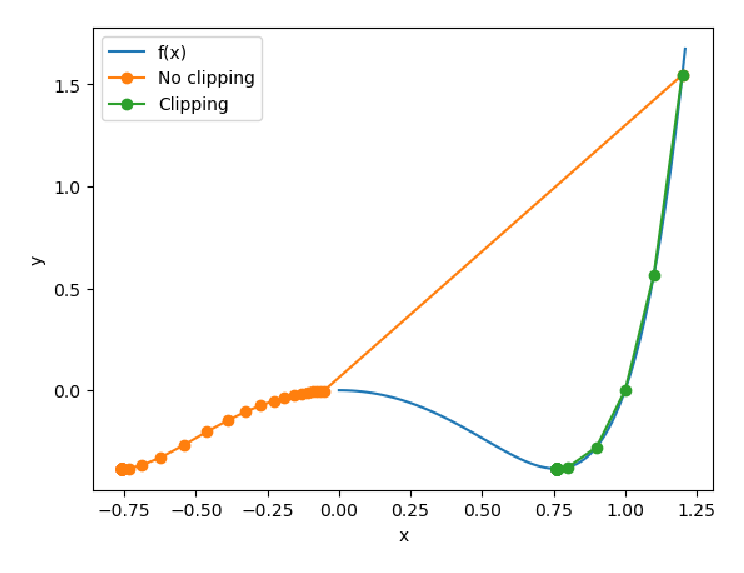
\includegraphics[scale=0.6]{pegado11}
\par\end{center}

Here, we can observe how if we don't clip, the gradient is too large
and we miss the minimum at the right, while clipping enables us to
get ther easily.

\paragraph{Gradient with Momentum}

Momentum represents an acceleration method for stochastic gradient
descent. The idea is to smooth gradient steps with some momentum or
inertia, using previous gradient steps as a ``\emph{memory}'' of
the direction.

Let's call the gradient at step $t$, $G^{t}\left(\theta\right)$,
then we define the velocity, $v^{t}\left(\theta\right)$, as
\[
v^{t}\left(\theta\right)=\alpha v^{t-1}\left(\theta\right)-\left(1-\alpha\right)G^{t}\left(\theta\right),
\]
 where $0\leq\alpha<1$ is a parameter controlling how much of the
gradient we use for the parameter update, usually set as 0.9. If it
is set to 0, we obtain the vanilla SGD.

The updates are done as
\[
\theta^{t+1}=\theta^{t}-\eta v^{t}\left(\theta\right),
\]
 where $\eta$ is the learning rate.

The momentum approach is shown below, observing a slight speedup.
\begin{center}
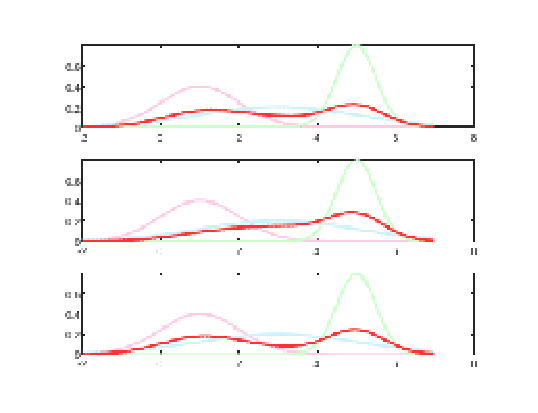
\includegraphics[scale=0.6]{pegado15}
\par\end{center}

\paragraph{Nesterov Momentum}

This represents a variant of gradient descent with momentum. It tries
to address the problem of the momentum approach, which is that is
tends to oscillate around the minimum. Nesterov corrects these oscillations
by estimating the gradient after the momentum update as:
\[
v^{t}\left(\theta\right)=\alpha v^{t-1}\left(\theta\right)-\left(1-\alpha\right)G\left(\theta-\alpha v^{t-1}\left(\theta\right)\right).
\]

\includegraphics[scale=0.6]{pegado16}

We can observe how the oscillations are less prominent. If the function
was different and momentum oscillates around the minimum, Nesterov
would help with this.

\paragraph{Dynamic Learning Rate}

Stochastic gradient descent estimates the gradient with only one sample,
and iterates over the whole dataset, as
\[
\theta\leftarrow\theta-\eta G\left(\theta;x^{i},y^{i}\right).
\]
 It is common to use minibatches instead:
\[
\theta\leftarrow\theta-\eta G\left(\theta;x^{i_{0}:i_{0}+B},y^{i_{0}:i_{0}+B}\right)=\theta-\eta\nabla_{\theta}\sum_{i=i_{0}}^{i_{0}+B}L\left(\theta;x^{i},y^{i}\right).
\]
 The learning rate is very important, and in fact it should decrease
during training, as we get closer to the optimum. Some reasons to
make this decrease are:
\begin{itemize}
\item True gradients becomes small when $\theta$ is close to the minimum.
\item With SGD, estimating the gradient with samples introduces noise, and
these gradients don't necessarily decrease.
\item A sufficient condition for convergence of SGD is:
\[
\sum_{k=1}^{\infty}\eta_{k}=\infty,\ and\ \sum_{k=1}^{\infty}\eta_{k}^{2}<\infty.
\]
\end{itemize}
In practice, what we do is apply a linear decay until some point $\tau$,
and keep it constant after this point:
\[
\eta_{k}=\left(1-\frac{k}{\tau}\right)\eta_{0}+\frac{k}{\tau}\eta_{\tau},
\]
 and $\eta_{\tau}$ after $\tau$ iterations.

Now, the question is, how to choose $\eta_{0},\eta_{\tau}$ and $\tau$?
There are several options:
\begin{itemize}
\item With trail and error (using train/validation sets).
\item It's better to monitor the loss function during training.
\item A practical choice:
\begin{itemize}
\item Choose $\tau$ so that the whole training dataset is seen around 100
times.
\item Choose $\eta_{\tau}$ around 1\% of $\eta_{0}$.
\item $\eta_{0}$ comes with experience:
\begin{itemize}
\item Too big: big variations in loss
\item Too small: learning is slow, we can get stuck in a plateau
\end{itemize}
\item Recipe:
\begin{itemize}
\item Try multiple $\eta_{0}$ over 100 iterations
\item Pick $\eta_{0}$ slightly higher than the best
\end{itemize}
\end{itemize}
\end{itemize}

\paragraph{Cyclical Learning Rate}

Optimization difficulties comes more from plateaus than from bad local
optima, and increasing $\eta$ allows to go across these plateaus.
For this, what is done is varying the learning rate in a cyclical
manner, from a minimum bound, $\eta_{min}$ to a maximum bound, $\eta_{max}$.

\paragraph{Super Convergence with One-Cycle Policy}

Only once cycle works as:
\begin{itemize}
\item Start with a small learning rate to begin convergence.
\item Increases and then stabilizes to high value, to cross big plateaus.
\item Decreases to a small value, to optimize local minima.
\end{itemize}
\begin{center}
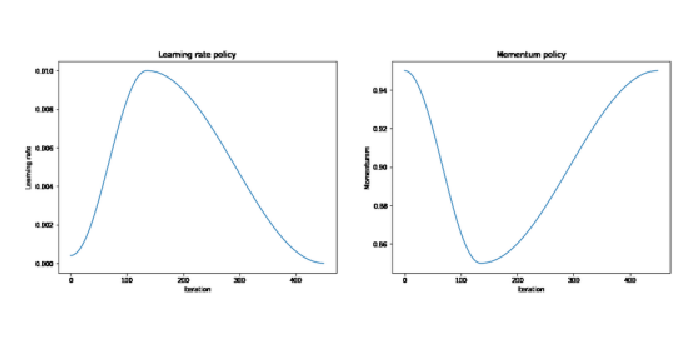
\includegraphics{pegado17}
\par\end{center}

\paragraph{SGD with Adaptive Learning Rates}

Preconditioning:
\[
\theta^{t+1}\leftarrow\theta^{t}-\eta_{t}P_{t}^{-1}G\left(\theta^{t}\right),
\]
 where $P_{t}$ can be defined in different ways. Let's see AdaGrad
and RMSProp.

\textbf{AdaGrad}: parameters with largest partial derivatives should
have a rapid decrease.
\[
P_{t}=\left[diag\left(\sum_{j=0}^{t}G\left(\theta^{t}\right)G\left(\theta^{t}\right)^{T}\right)\right]^{\frac{1}{2}}.
\]
 More precisely:
\[
\begin{cases}
g^{t}\leftarrow G\left(\theta^{t}\right)\\
r^{t}\leftarrow r^{t-1}+g^{t}\odot g^{t}\\
\theta^{t+1}\leftarrow\theta^{t}-\frac{\lambda}{\delta+\sqrt{r^{t}}}\odot g^{t}
\end{cases}
\]

AdaGrad converges quickly on convex problems. However, keeping all
the history with momentum can be detrimentary, and smoothing the gradient
destroys information. 

RMSProp: introduces momentum when computing the precondicioner. The
idea is to adapt the learning rate to the curvature of the loss function,
putting the brakes on when the function is steep and accelerating
when the loss function is flat.
\[
P_{t}=\left[diag\left(\alpha P_{t-1}+\sum_{j=0}^{t}G\left(\theta^{t}\right)G\left(\theta^{t}\right)^{T}\right)\right]^{\frac{1}{2}}.
\]


\paragraph{More precisely:
\begin{align*}
v^{t}\left(\theta\right) & =\alpha v^{t-1}\left(\theta\right)+\left(1-\alpha\right)G\left(\theta\right)^{2}\protect\\
\theta^{t+1} & =\theta^{t}-\frac{\eta}{\epsilon+\sqrt{v^{t}\left(\theta\right)}}G\left(\theta\right).
\end{align*}
 Adam}

Adam (Adaptative Moment Estimation) builds on RMSProp, but also uses
a moving average of the gradients. It works as:
\begin{align*}
m^{t}\left(\theta\right) & =\beta_{1}m^{t-1}\left(\theta\right)+\left(1-\beta_{1}\right)G\left(\theta\right)\\
v^{t}\left(\theta\right) & =\beta_{2}v^{t-1}\left(\theta\right)+\left(1-\beta_{2}\right)G\left(\theta\right)^{2}\\
\theta^{t+1} & =\theta^{t}-\eta\frac{m\left(\theta\right)}{\epsilon+\sqrt{v\left(\theta\right)}}.
\end{align*}
 In practice, Adam is the most used optimizer. However, there are
more efficient algorithm, like LARS (Layerwise Adaptive Rate Scaling)
or LAMB (LARS+Adam).

\paragraph{Comparison}
\begin{itemize}
\item SGD momentum should allow for better solution, but hyperparameters
are harder to find.
\item Adam is easier to tune.
\end{itemize}

\subsection{Initialization and Normalization}

The parameters of a deep learning model need initial values. The assignation
of initial values is called \textbf{initialization}, and can impact
the optimization process in several ways:
\begin{itemize}
\item A bad initialization can make the training process not to converge.
\item It can impact the convergence quality, in terms of speed and the value
reached.
\item Also, it can impact the generalization error.
\end{itemize}
Therefore, a difficult question arises: initial parameters can help
optimization, but can detriment the generalization error.

\begin{tcolorbox}
\textbf{Principle: Break Symmetries}

Two identical parameters, connected to the same input, should be initialized
differently, to incentivize different learning.
\end{tcolorbox}

One option could be to initialize everything to 0, but this is not
a good choice, because it disentivizes learning. Instead, there are
different initialization schemes, like random initialization.

\subsubsection{Random Initialization}

Random initialization uses a probability distribution to initialize
the weights. For example, \textbf{Xavier initialization} uses an uniform
distribution as
\[
W_{i,j}\sim U\left(-\frac{\sqrt{6}}{\sqrt{n_{i}+n_{i+1}}},\frac{\sqrt{6}}{\sqrt{n_{i}+n_{i+1}}}\right),
\]
 where $n_{j}$ is the number of neurons in layer $j=1,...,N$. The
input layer is initialized as
\[
W_{0,j}\sim\mathcal{N}\left(0,\sqrt{\frac{2}{n_{1}}}\right).
\]


\subsubsection{Input normalization}

Gradient descent is sensitive to strong variations in the input, and,
ideally, the surface of the loss function should ahve a uniform curvature
in all directions, similar to a sphere. This can be incentivized by
input normalization, i.e., normalizing all input parameters so that
they all lie in a similar value range.

Moreover, there is the concept of \textbf{batch normalization}, or
adaptive reparametrization. This consists in normalizing the input
of each layer of a neural network. It is motivated by the following:
\begin{itemize}
\item Deep neural networks are compositions of functions, whose parameters
are iteratively updated during training.
\item The updates are done simultaneously to all layers, and unexpected
effects can come into play, since each layer is updated assuming all
other layers remain constant.
\item Therefore, the updates to other layers can add high order effects
that can lead to the problem of \textbf{gradient explosion}, a situation
in which the gradient keeps growing indefinitely.
\end{itemize}
In this case, the idea is to normalize the distribution of each input
feature in each layer, across each minibatch, to a normal, $\mathcal{N}\left(0,1\right)$:
\begin{align*}
\mu & \leftarrow\frac{1}{m}\sum_{i=1}^{m}\overline{x}^{i},\\
\sigma^{2} & \leftarrow\frac{1}{m}\sum_{i=1}^{m}\left(\overline{x}^{i}-\mu\right)^{2},\\
\overline{x}^{i} & \leftarrow\frac{\overline{x}^{i}-\mu}{\sqrt{\sigma^{2}-\varepsilon}}.
\end{align*}
 Remember that $\varepsilon$ is the approximation of the generalization
error, $\varepsilon=\frac{VC_{dim}}{N}$.

\subsection{Regularization}

The loss function can be small on the training data, but large on
the dataset. This is the overfitting problem, that we have seen before.
Deep NN can tend to overfit, since more depth implies more free parameters,
and therefore a higher VC dimension, which can increase $\varepsilon$
according the rule of thumb for its approximation. 

A way to go around this is to put constraints on the weights, to reduce
the VC dimension. This can be done through regularization.

\subsubsection{$\mathcal{L}_{2}$ Regularization (or Ridge)}

$\mathcal{L}_{2}$ regularization keeps the $\mathcal{L}_{2}$ norm
of the free patameters, $\left\Vert \theta\right\Vert $, as small
as possible, during learning.

The intuition is that each neuron will use all its inputs with small
weights, instead of specializing on a small part with high weights.

To accomplish this, we have to minimize two things at the same time:
the training loss and a penanlty term representing the norm of the
weights:
\[
\mathcal{J}\left(\theta\right)=\mathbb{E}_{D}\left[\left\Vert t-y\right\Vert ^{2}\right]+\lambda\left\Vert \theta\right\Vert ^{2},
\]
 where $\lambda$ is the \textbf{regularization parameter}, controlling
the strength of the regularization:
\begin{itemize}
\item If $\lambda$ is small, there is only a small regularization, allowing
higher weights.
\item If $\lambda$ is high, the weights will be kept very small, but they
may not minimize the training loss.
\end{itemize}
The gradient of this new loss function is
\[
\nabla_{\theta}\mathcal{J}\left(\theta\right)=-2\left(t-y\right)\nabla_{\theta}y+2\lambda\theta,
\]
 and so the parameter updates become
\[
\Delta\theta=\eta\left(t-y\right)\nabla_{\theta}y-\eta\lambda\theta.
\]
 The $\mathcal{L}_{2}$ regularization leads to weights decay: even
if there is no output error, the weight will converge to 0, forcing
the weights to constatly learn, and disincentivizing the specialization
on particular examples (overfitting), enhancing generalization.

\subsubsection{$\mathcal{L}_{1}$ regularization (or Lasso)}

In this case, we penalize the absolute value of the weights, instead
of their euclidean norm:
\[
\mathcal{J}\left(\theta\right)=\mathbb{E}_{D}\left[\left\Vert t-y\right\Vert ^{2}\right]+\lambda\left\Vert \theta\right\Vert _{1}.
\]
 This method leads to very sparse representations, where a lot of
neurons may be inactive, and only a few represent the input.

\subsubsection{Early Stopping}

During training, a common behavior is the following:
\begin{center}
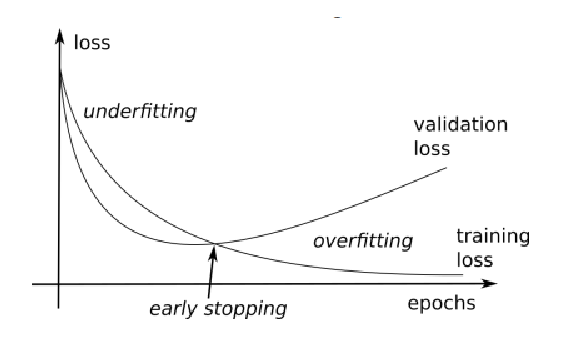
\includegraphics[scale=0.6]{pegado18}
\par\end{center}

It's usual that the training error decreases constantly, while the
validation error decreases, and the increases again. If we manage
to find the optimal point in this process, we can stop earlier the
training process, before the validation error gets larger.

This method is equivalent to $\mathcal{L}_{2}$ normalization, both
limiting the capacity of the model:
\begin{itemize}
\item With Ridge regularization, small slope regions contract the dimension
of $\theta$, which decays to 0, and high slope regions are not regularized
because they help descent.
\item With early stopping, parameters with high slope are learned before
parameters with low slope.
\end{itemize}

\subsubsection{Dropout}

Dropout considers all the networks can be formed by removing some
units from a network. With this in mind, the method consists of:
\begin{itemize}
\item At each optimization iteration: we apply random binary masks on the
units to consider.
\end{itemize}
The probability of dropout, $p$, is a hyperparameter. Therefore,
what we do at training time is, at each step, deactivate some neurons,
randomly. This incentivizes generalization, since relying on some
neurons specializing a lot for some features of the training data
is harder if these neurons are not always available. 

Note that, at inference time, all neurons are always available.

\subsubsection{Data Augmentation}

The best way to avoid overfitting is collecting more data, but this
can be hard, costly, or simply impossible. A simple trick is \textbf{data
augmentation}, which consists in creating new varied data from the
current data by perturbing it, while not chaning the labels associated
to it.

For example:
\begin{center}
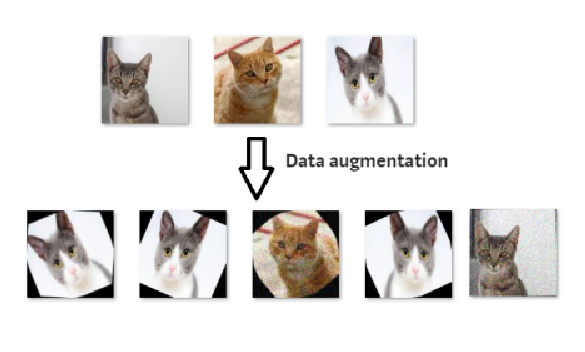
\includegraphics[scale=0.6]{pegado19}
\par\end{center}

\textbf{Mixup} is a particular case of data augmentation, consisting
on creating new training new samples with labels by interpolation:
\begin{align*}
\hat{x} & =\lambda x_{i}+\left(1-\lambda\right)x_{j},\\
\hat{y} & =\lambda y_{i}+\left(1-\lambda\right)y_{j},
\end{align*}
 where $\lambda\sim Beta\left(\alpha,\alpha\right)$, with $\alpha\in\left[0.1,0.4\right]$
for classification tasks. This method works for structured data, and
can be used to stabilizing GANs (we will see this later).

\subsection{Vanishing Gradients}

Contrary to what we could think, adding more layers to a DNN does
not necessarily lead to better performance, both on the training and
test set. For instance, see the following graph, where we observe
the performance of a 20 layers NN (left) and a 56 layers NN (right):
\begin{center}
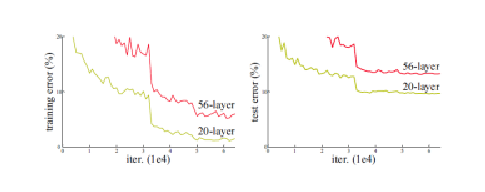
\includegraphics{pegado20}
\par\end{center}

We observe how its performance is worse in all senses. The main reason
for this is the \textbf{vanishing gradient problem}. The gradient
of the loss function is repeatedly multiplied by a weight matrix $W$
as it travels backwards in a deep NN, as
\[
\frac{\partial h_{k}}{\partial h_{k-1}}=f'\left(W^{k}h_{k-1}+b^{k}\right)W^{k}.
\]
 When the gradient arrives to the first layer, the contribution of
the weight matrices is comprised between $W_{min}^{d},$ and $W_{max}^{d}$,
which are the weight matrix with the highest and lowest norm, and
$d$ is the depth of the network. We find:
\begin{itemize}
\item If $\left|W_{max}\right|<1$, then $W_{max}^{d}$ is very small for
high values of $d$, and the gradient vanishes.
\item If $\left|W_{min}\right|>1$, then $W_{min}^{d}$ is very high for
high values of $d$, and the gradient explodes.
\end{itemize}
We saw that exploding gradients can be solved by gradient clipping.
But vanishing gradients are still the current limitation of deep NN.
The solutions include the utilization of ReLU activaiton functions,
unsupervised pre-training, batch normalization, residual networks,
etc.

\subsubsection{Residual network}

A Residual Neural Network, or \textbf{ResNet}, is an advanced type
of neural network that is specifically designed to help improve the
performance of deep learning models.

ResNet introduces the concept of residual learning. Instead of expecting
each stack of layers to directly fit a desired underlying mapping,
ResNet layers are designed to fit a residual mapping. The key component
of ResNet is the introduction of \textquotedbl skip connections\textquotedbl{}
or \textquotedbl shortcuts\textquotedbl{} that bypass one or more
layers. A skip connection in a ResNet allows the gradient to be directly
backpropagated to earlier layers.

These skip connections perform identity mapping, and their outputs
are added to the outputs of the stacked layers. This design helps
in training deeper networks by mitigating the vanishing gradient problem.
With residual blocks, the network learns the additive residual function
with respect to the layer inputs, making it easier to optimize and
gain accuracy from considerably deeper networks.
\begin{center}
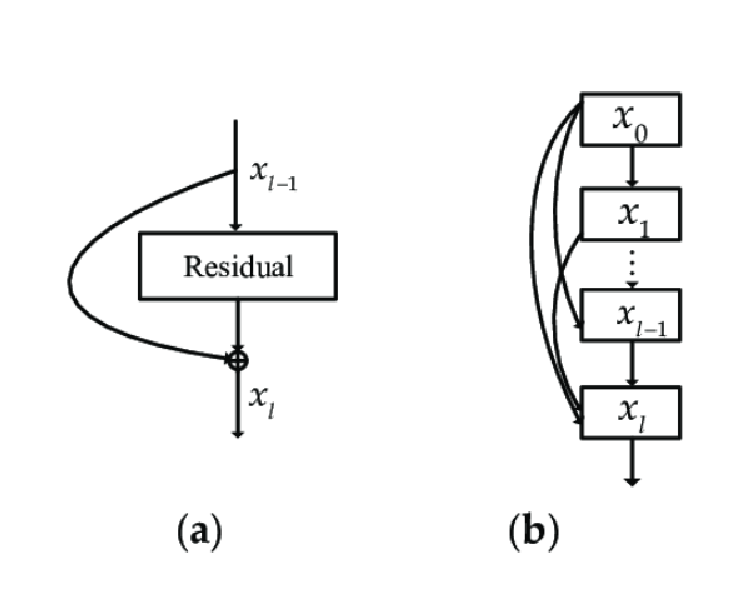
\includegraphics{pegado21}
\par\end{center}

\subsubsection{Stochastic Depth}

Stochastic depth is a training technique for deep neural networks,
particularly effective for very deep networks like ResNets. It was
introduced as a solution to the problem of vanishing gradients and
long training times in deep networks.

During training, stochastic depth randomly drops layers in the network.
The idea is similar to dropout, where random neurons are turned off
during training to prevent overfitting. In stochastic depth, however,
it's entire layers that are dropped.

Each training iteration uses a shallower version of the network. The
depth of the network varies each time, as different subsets of layers
are randomly deactivated.

Notice how stochastic depth is particularly useful for ResNets, where
skip connections (or residual connections) are a key feature. When
a residual block is dropped, the skip connection effectively takes
its place, allowing the signal to still propagate forward.

At test time, all layers are used, but their outputs are scaled appropriately
to compensate for the dropout during training. This ensures that the
network can benefit from its full depth during inference.
\begin{center}
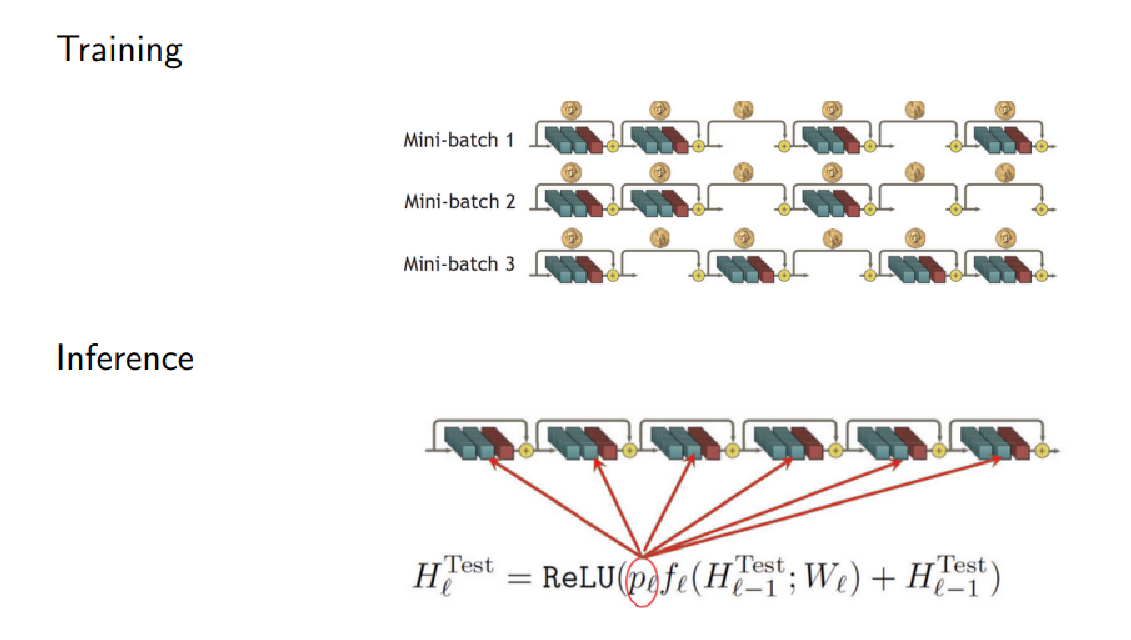
\includegraphics[scale=0.6]{pegado22}
\par\end{center}

\subsection{Double Descent}

Double descent is a phenomenon observed in the training of machine
learning models, particularly in relation to the model's complexity
and its performance on a given task. This concept challenges the traditional
understanding of the bias-variance tradeoff and has gained attention
in the field of machine learning and statistics.

The double descent curve shows that after the point where the model
starts to overfit (as per the traditional U-shaped bias-variance tradeoff
curve), increasing the model complexity even further can lead to a
decrease in the total error again.

It shows the following phases:
\begin{itemize}
\item \textbf{Underparameterized Regime}: Where the model has too few parameters
and underfits the data. Here, increasing complexity reduces bias and
total error. 
\item \textbf{Interpolation Threshold}: At this point, the model just starts
to fit all the training data perfectly (including noise), leading
to high variance and total error. 
\item \textbf{Overparameterized Regime}: Beyond this threshold, as complexity
continues to increase, the model enters the second descent where surprisingly,
the total error begins to decrease again despite the model being overparameterized.
\end{itemize}
The double descent phenomenon is especially noticeable in scenarios
with limited training data. With more data, the peak of the curve
(at the interpolation threshold) becomes less pronounced.

Double descent suggests that in some cases, choosing an even more
complex model after hitting the overfitting point can improve performance.

For example, observe this phenomenon in the following graphs:
\begin{center}
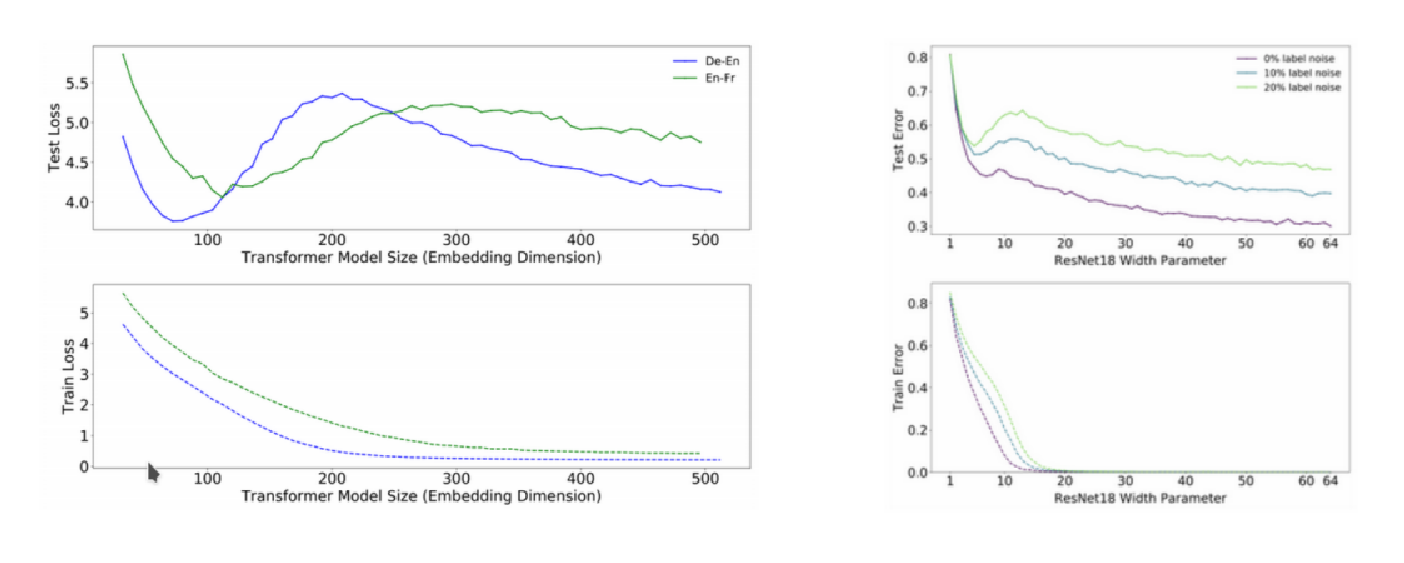
\includegraphics[scale=0.6]{pegado23}
\par\end{center}

A similar phenomenon is \textbf{grokking}, which occur when we increase
training time. It is remarkable that shallow models don't show it,
which is a reason to use deep networks! 
\begin{center}
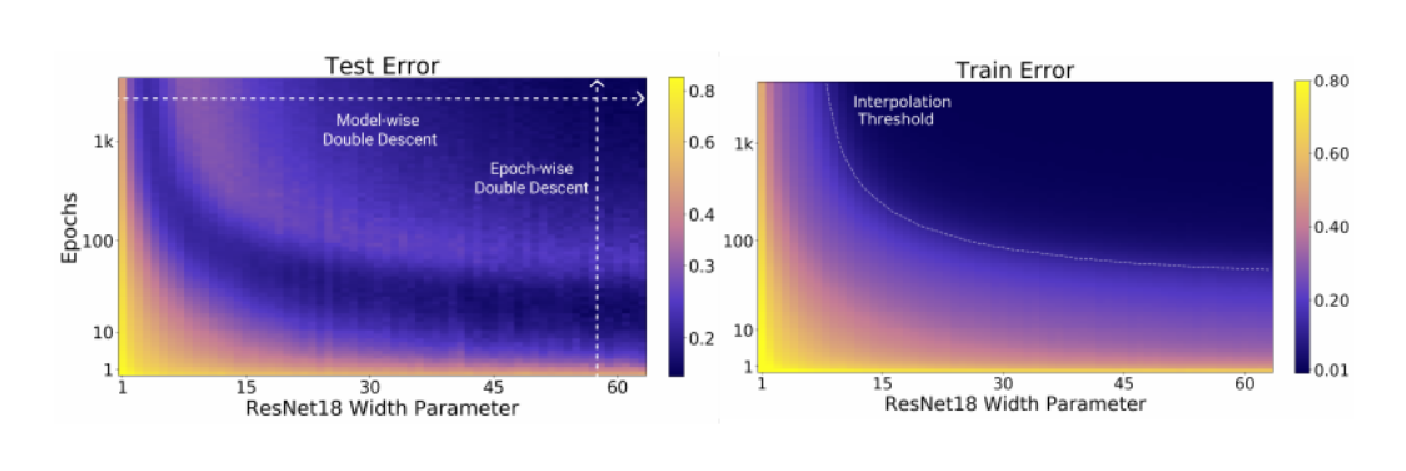
\includegraphics[scale=0.6]{pegado24}
\par\end{center}

\section{Convolutional Neural Networks}

\subsection{Introduction}

When working with MLP, we find several limitations:
\begin{enumerate}
\item Dealing with data with a high number of features. For example, let
imagine we are working with a dataset of images at full HD resolution.
The feature size is $1920\times1080\times3=6\ 220\ 800$. Learning
a single layer to reduce the dimension to 1000 requires around $6000K\times1K\sim10^{9}$
parameters, making the training really difficult.
\item Use the knowledge of the input data modality to shape the network.
E.g., for images, the network should be equivariant to translation.
This means that a pattern should be detected independently of where
it is located in the image.
\end{enumerate}
\textbf{Convolutional Neural Networks (CNNs)} appear to mitigate these
limitations.

\begin{tcolorbox}
\begin{defn}
A CNN is an NN that uses convolutions in place of general matrix multiplication
in, at least, one of their layers.
\end{defn}
\end{tcolorbox}

CNNs deal with data arranged according to a grid, which can be temporal
date, images, videos, etc.

\subsubsection{History of CNNs}
\begin{itemize}
\item The first work on CNNs was done in 1998, by LeCun et al. 
\item Theoretical advances to make DNN converge by Hinton et al. in 2006.
\item Access to large datasets such as ImageNet thanks to Deng et al. in
2009.
\item Advances in hardware technology to scale learning, with better CPUs
and the development of GPUs.
\item Win of the 2012 ImageNet challenge with AlexNet, using CNNs, by Krizhevsky
et al. in 2012, made them famous.
\end{itemize}

\subsection{Convolutions}

\begin{tcolorbox}
\begin{defn}
Given two functions, $f,g:\mathbb{R}\rightarrow\mathbb{R}$, their
\textbf{convolution} is defined as
\[
\left(f*g\right)\left(x\right)=\int_{-\infty}^{\infty}f\left(z\right)g\left(x-z\right)dz.
\]
 For discrete function, it becomes
\[
\left(f*g\right)\left(m,n\right)=\sum_{i,j=-\infty}^{i,j=\infty}f\left(i,j\right)g\left(m-i,n-j\right),
\]
 where in this case $f$ and $g$ are bidimensional.

$f$ is called the \textbf{input} \textbf{signal}.

$g$ is called the \textbf{kernel}, or filter.

$f*g$, the convolution output, is the \textbf{feature map}.
\end{defn}
\end{tcolorbox}

\begin{rem}
Properties of convolutions:
\begin{itemize}
\item Commutativity:
\[
\left(f*g\right)\left(x\right)=\left(g*f\right)\left(x\right).
\]
\item Distributivity:
\[
\left(f*\left(g+h\right)\right)\left(x\right)=\left(f*g\right)\left(x\right)+\left(f*h\right)\left(x\right).
\]
\item Associativity:
\[
\left(\left(f*g\right)*h\right)\left(x\right)=\left(f*\left(g*h\right)\right)\left(x\right).
\]
\end{itemize}
\end{rem}
%
\begin{rem}
Observe that convolutions can be understood as taking a moving average
of $f$ around each point $x$, with weights provided by $g$. If
$\int gdx=1$, then it would represent a proper moving average.
\end{rem}
In practice, however, CNNs do not really use convolutions, but \textbf{cross-correlations},
which consist in sliding one signal (or function) over another and
measuring the similarity at each position. It's a way to track how
much one signal resembles another as you shift one of them over time
or space. Their definition is very similar to convolutions, but convolutions
invert the kernel function, while cross-correlations do not:
\[
\left(f\logof g\right)\left(m,n\right)=\sum_{i,j=-\infty}^{i,j=\infty}f\left(m,n\right)g\left(m+i,n+i\right).
\]

While MLPs make an interaction between each input neurons and each
output neurons, CNNs have \textbf{sparse interactions}, thanks to
the kernels, which have a small number of parameters, significantly
reducing the number of parameters of the network.

Moreover, in MLP there is one weight per connection between the input
and the output, while CNNs apply the same kernel to different parts
of the input, also reducing the number of parameters of the network.
This is called the \textbf{parameter sharing} property.

\begin{tcolorbox}
\begin{defn}
A function $f$ is said to be \textbf{equivariant} to a transform
$g$, if for any input $x$, it holds
\[
f\left(g\left(x\right)\right)=g\left(f\left(x\right)\right).
\]
\end{defn}
\end{tcolorbox}

Because of paratemer sharing, the CNNs are equivariant to translations.
This makes them particulary useful for some modalities, such as image,
for which we aim to detect several objects in the same manner.

Images, and some other modalities, like videos, are composed of \textbf{channels}.
For example, RGB is a 3-channel way to compose images.

Kernels are convoluted with all channels of the input, as visualized
in the following figure.

\begin{figure}
\begin{centering}
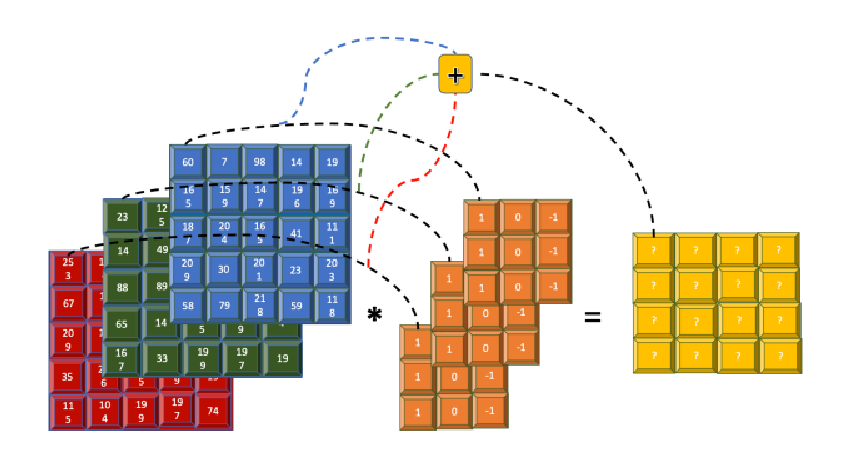
\includegraphics[scale=0.6]{pegado28}
\par\end{centering}
\caption{Convolution of a 3-channel input with a 3-channel kernel.}
\end{figure}

Convolutions are not equivariant to rotation, zoom, etc. And these
might be interesting for our model to be invariant. To make the network
invariant to such transformation, we can transform the data with data
augmentations including zooming and rotating, and feeding the network
with this transformed data.

Notice how convolutions can reduce the input size, whenever the kernel
is larger than $1\times1$. This is due to the necessity to fit the
whole image. 

The output size of the convolution of an input of size $n_{h}\times n_{w}$
with a kernel of size $k_{h}\times k_{w}$ is
\[
\left(n-k_{h}+1\right)\times\left(n_{w}-k_{w}+1\right).
\]


\subsubsection{Fixed Kernels Weights}

If we are interested in certain features, and we know how to define
a kernel that is good for identifying these features, we can just
do this and applying this kernel.

For example, in the following illustration we observe a kernel that
is good at finding vertical edges:
\begin{center}
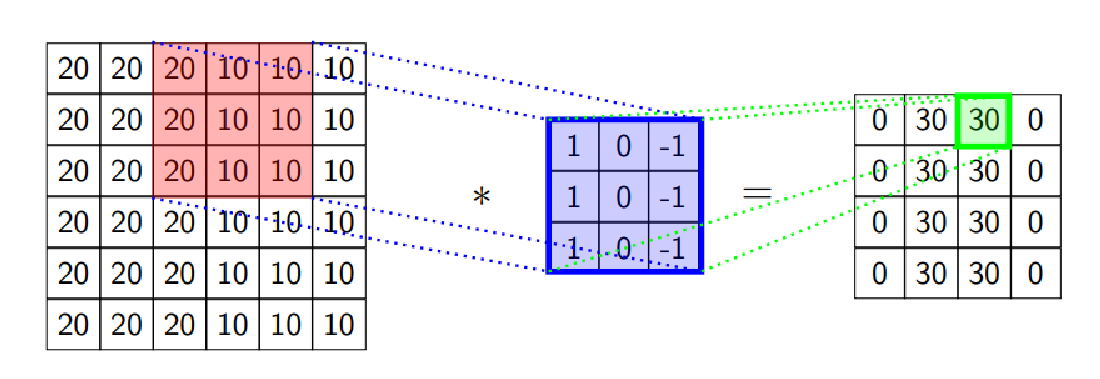
\includegraphics[scale=0.6]{pegado29}
\par\end{center}

\subsubsection{Learned Kernel Weights}

Learning a CNN backbone using DL is learning the weights of the kernels
via backpropagation. The filters seek to learn the best representation
to fit its training objective, via the training loss.

Using different kernels allows to detect various patterns, so usually
CNNs contain thousands of kernels and are grouped in hierarchical
layers, to learn from low-level features to high-level features.

To compute various features, such as different detections (horizontal,
vertical, diagonal, etc.) we need several filters. For an input of
size $C\times n_{1}\times n_{2}$, where $C$ is the amount of channels,
and $F$ filters of size $C\times m_{1}\times m_{2}$, the feature
map produced has $F$ channels and is of size
\[
F\times\left(n_{1}-m_{1}+1\right)\times\left(n_{2}-m_{2}+1\right).
\]


\subsubsection{Receptive fields}

The \textbf{receptive field} is the region of the input space that
a particular CNN's feature is looking at.

\subsubsection{$1\times1$ Convolution}

The $1\times1$ convolution is a linear combination of all channels
for each pixel, allowing to learn to reduce or increase the number
of filters.

In general, if the input is of size $F_{in}\times H\times W$ and
the filter is of size $F_{out}\times1\times1$, then
\begin{itemize}
\item If $F_{out}<F_{in}$: the dimension is reduced.
\item If $F_{out}>F_{in}$: the dimension is increased.
\end{itemize}
$1\times1$ convolutions can replace fully connected layers. For example,
in classification, we could do $F_{out}=N_{classes}$.

\subsection{Padding, Stride, Pooling}

\subsubsection{The Sides Problem}

Convolutions are applied on fixed size patches of the input data,
and they can only be shifted until there are no pixels. This introduces
two potential problems:
\begin{itemize}
\item The output size is reduced.
\item The information in the sides of the image can be lost, because the
convolution cannot be applied there.
\end{itemize}

\subsubsection{Padding}

Padding is a solution to the edge problem, consisting on adding data
at the sides of the image. There are several strategies, but in general,
we just add zeros:
\begin{center}
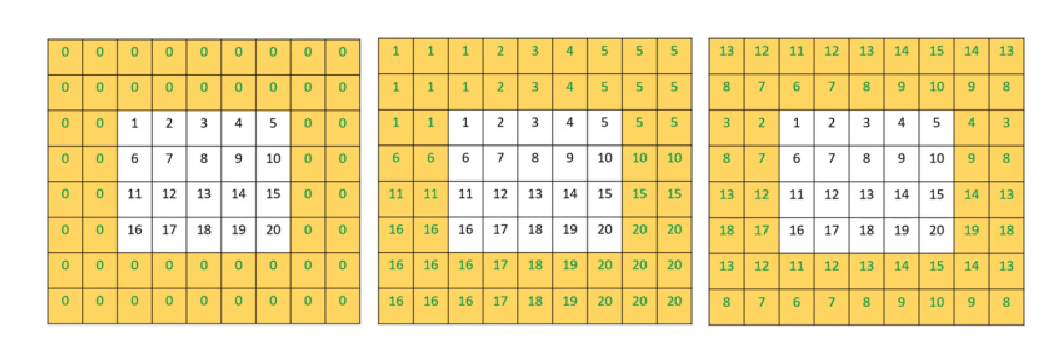
\includegraphics[scale=0.6]{pegado30}
\par\end{center}

There are several modes of zero padding. For a padding of $k$ pixels:
\begin{itemize}
\item Valid: no padding.
\item Same: add $\frac{k-1}{2}$ zeros on each side.
\item Full: add $k$ zeros on each side.
\end{itemize}
The output size of a convolution of a $n_{h}\times n_{w}$ sized input,
to which we add $p_{h}$ rows and $p_{w}$ columns of padding, and
a kernel of size $k_{h}\times k_{w}$ becomes
\[
\left(n_{h}-k_{h}+p_{h}+1\right)\times\left(n_{w}-k_{w}+p_{w}+1\right).
\]
 Generally, we want to have $p_{h}=k_{h}-1$ and $p_{w}=k_{w}-1$,
which is achieve by applying same zero padding.

\subsubsection{Stride}

As far as we have seen, we slide the kernel across all locations right
and down. However, we could skip some of this locations, effectively
reducing the feature map output and the computational cost, but at
the expense of the accuracy of the representations.

If we add $s_{h},s_{w}$ for the height and width strides, the feature
map size is
\[
\frac{\left(n_{h}-k_{h}+p_{h}+1+s_{h}\right)}{s_{h}}\times\frac{\left(n_{w}-k_{w}+p_{w}+1+s_{w}\right)}{s_{w}}.
\]


\subsubsection{Pooling}

Pooling consists in statistically summarizing a neighbourhood. A pooling
layer takes a window of values and output one value. There are several
pooling types:
\begin{itemize}
\item Max Pooling: take the maximum value of a window.
\item Average pooling: take the eman value of a window.
\item $L_{2}$ norm, weighted average pooling, etc.
\end{itemize}
For example, the following illustrates the use of a 2x2 max pooling
layer:
\begin{center}
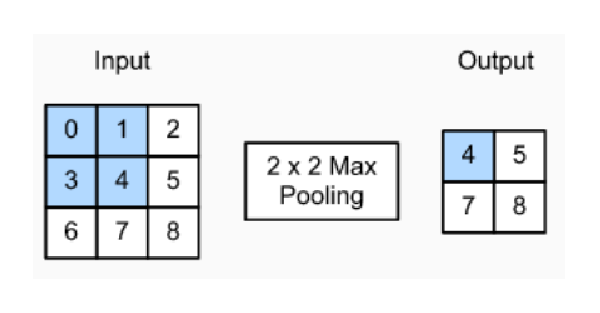
\includegraphics[scale=0.6]{pegado31}
\par\end{center}

Pooling is useful to make our representations invariant to minor translations.
For deep layers, minor modifications can mean great changes in the
input image.

Also, it reduces the amount of parameters and computation, and help
reducing overfiting.

It sets up a strong prior: invariance to local translation of learned
kernels.

It can be degrading for some tasks, where precise locations are required.

\subsection{CNNs}

\textbf{LeNet} by LeCun et al. in 1998 was designed after 10 uears
of working with handwritten bank checks. It paved the basics of DL:
\begin{itemize}
\item Feature extraction by convolution layers.
\item Classification by MLP layers.
\item Layer of convolution followed by average pooling, and non-linearity,
with sigmoid or tanh.
\item SGD optimizer to perform backpropagation.
\end{itemize}
The architecture is the following:
\begin{center}
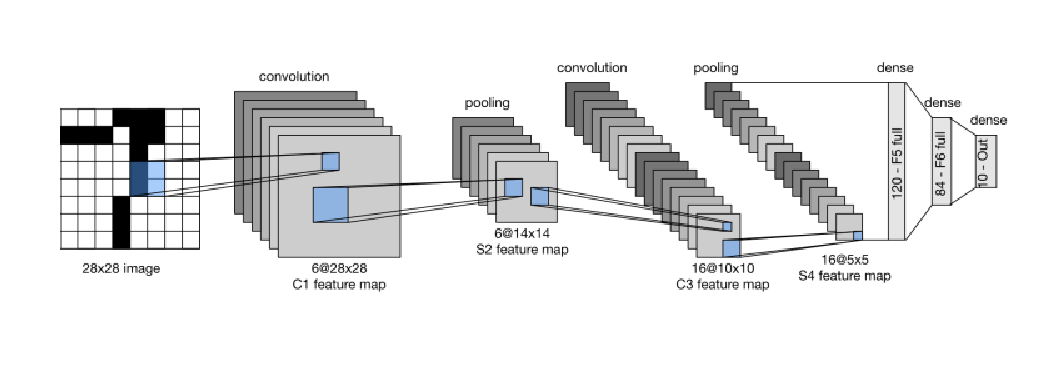
\includegraphics[scale=0.6]{pegado32}
\par\end{center}

\textbf{AlexNet} by Krizhevsky et al. in 2012 was on of the first
DNN, and won the 2012 ImageNet challenge, causing a new DL area. They
extended LeNet to larger images, with wider convolutions, and used
ReLUs and max pooling, combined with dropout.

A very interesting fact they observed was that as the layers were
deeper, the receptive field was higher: The first layers learn basic
patterns, while deeper layers learn more complicated shapes.
\begin{center}
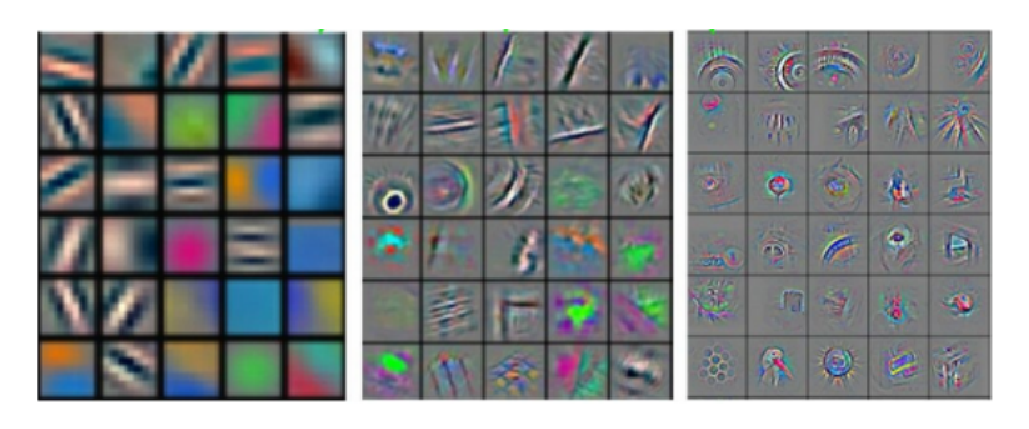
\includegraphics[scale=0.6]{pegado33}
\par\end{center}

\textbf{Visual Geometry Group (VGG)} by Simonyan et al. in 2015 was
the first network with blocks. the blocks consisted in:
\begin{itemize}
\item Convolution layer with padding to keep the same resolution.
\item Non-linearity.
\item Pooling layer to reduce resolution.
\end{itemize}
The architecture was the following:
\begin{center}
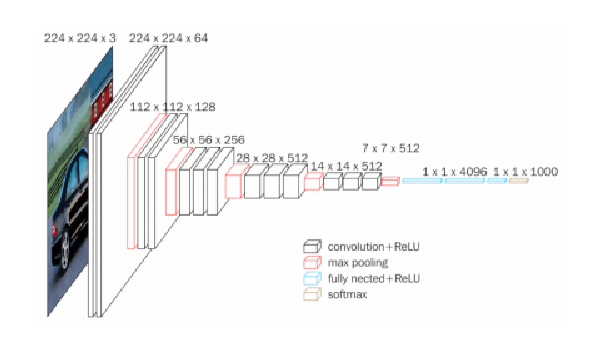
\includegraphics[scale=0.6]{pegado34}
\par\end{center}

The problem was how to maintain enough resolution to have a lot of
blocks. The solution was to introduce more convolutions at low resolution,
instead of few convolutions at high resolution.

This increases the number of non-linearities and reduces the number
of parameter to achieve an equal receptive field.

\textbf{Network in Network (NiN)}, by Lin et al. in 2013: previous
architectures improved by enhacing the number of convolutions (width)
and deepening the network (depth). This presents two problems:
\begin{itemize}
\item The last fully connected layers consume large number of parameters.
\item It is difficult to add non-linearity without using fully connected
layers, that destroy the spatial structure.
\end{itemize}
NiN made improvements:
\begin{itemize}
\item It used $1\times1$ convolutiones to increase the number of non-linearities.
\item Also, a global average pool at the end to remove large fully connected
layers.
\end{itemize}
\textbf{Inception Blocks}: Google was facing a problem. They needed
fast deployment and inference, but large convolutions with lots of
channels increase inference time. Their solution was to reduce the
number of channels by applying several convolutions in parallel. Instead
of choosing a single filter size for a given layer, Inception blocks
apply multiple different-sized filters (e.g., 1x1, 3x3, 5x5 convolutions)
in parallel to the same input feature map. This allows the network
to capture information at various scales.

An inception block looks as follows:
\begin{center}
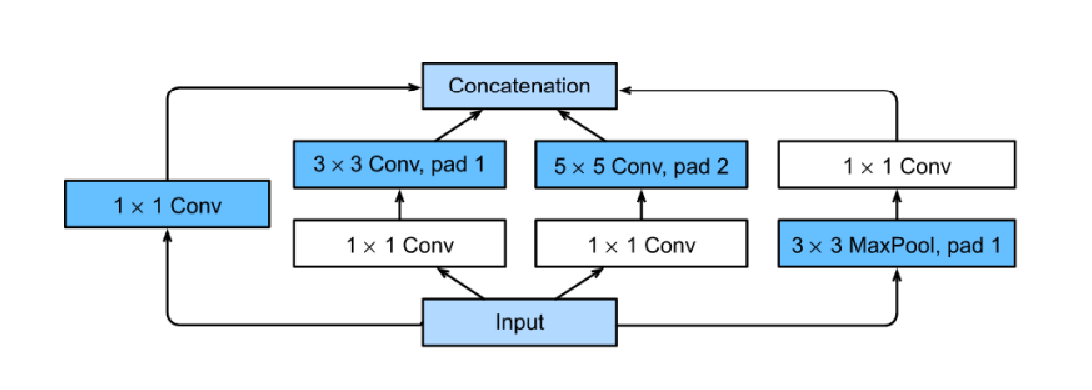
\includegraphics[scale=0.6]{pegado35}
\par\end{center}

\textbf{GoogleNet}, by Szegedy et al. in 2015 was based on inception
blocks. It used several classifiers throughout training to enhance
discriminative features at first layers, and reduce vanishing gradients.

\textbf{Residual Blocks}: these blocks make use of \textbf{residual
connections}, or shortcut connections, which forward the input to
the following layer. That is, if a layer is represented as $f\left(x\right)$,
the same layer, when used inside a residual block, would be $f\left(x\right)+x$.
This is illustrated below.
\begin{center}
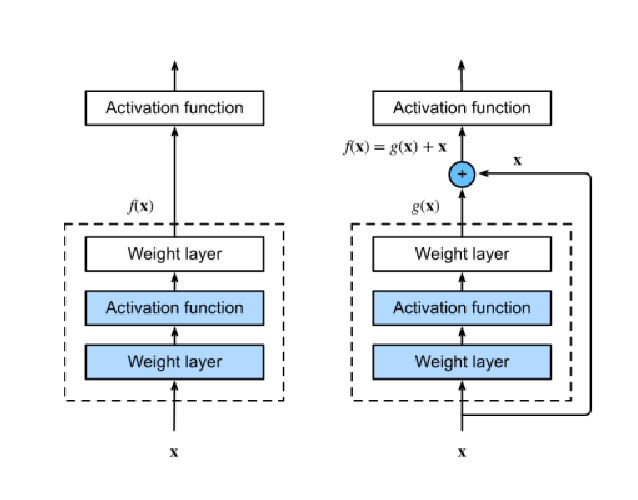
\includegraphics[scale=0.6]{pegado36}
\par\end{center}

Residual blocks make the identity function easier to learn, and reduce
vanishing or exploding gradient problems.

\textbf{ResNet Blocks}: these blocks are a combination of VGG blocks
and residual blocks. They use $3\times3$ convolutions, with batch
normalization to stabilize training and residual connection concatenated
to the result of applying two of these convolutions. The residual
connection can be either direct, or by means of a $1\times1$ convolution.
This is illustrated below:
\begin{center}
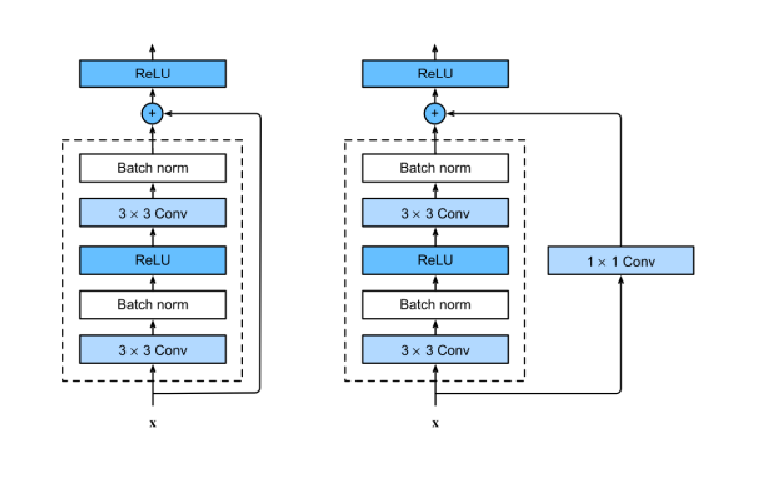
\includegraphics[scale=0.6]{pegado37}
\par\end{center}

\textbf{Residual Neural Networks (ResNet)}, by He et al. in 2016,
is a network architecture consisting of blocks of residual blocks.
There are different ResNets depending on how many blocks or layer
are used. For example, the following is a ResNet-18, as it has 18
trainable layers (the first 7x7 conv, two 3x3 convs for each internal
block, and there are eight of them, and the last fully connected layer):
\begin{center}
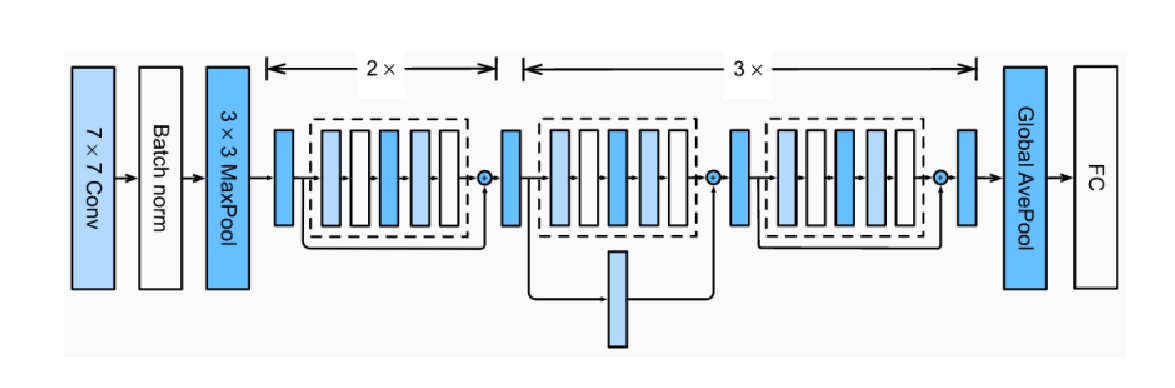
\includegraphics[scale=0.6]{pegado38}
\par\end{center}

ResNet is a widely used backbone until today.

\textbf{ResNexts: Group convolution}, by Xie et al. in 2017. To add
more non-linearities in ResNets we can add more layers, increase the
width of convolutions or the number of channels. However, increasing
the number of channels add quadratic complexity $\left(F_{in}\times F_{out}\right)$.
Group convolutions is a technique to reduce the computational complexity
while still increasing the network's width. In group convolution,
the input channels are divided into groups, and a convolution is performed
independently on each group. This means that if you have $g$ groups,
each group will have $\frac{c}{g}$ input channels and $\frac{b}{g}$
filters applied to it, where $c$ is the total number of input channels,
and $b$ is the total number of intermediate channels. Each filter
in a group only interacts with the input channels within that group.

The following diagram shows a block of the ResNeXt architecture. The
input channels are first split into $g$ groups. Each group is processed
by its own set of 1x1 convolutions (to reduce dimensionality), followed
by 3x3 convolutions (to capture spatial hierarchies). The outputs
of these groups are then concatenated, and a final 1x1 convolution
is applied to the concatenated result to produce the final output
channels.
\begin{center}
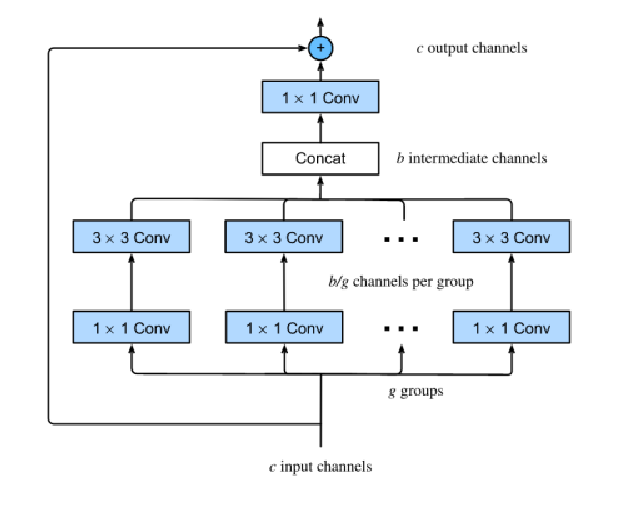
\includegraphics[scale=0.6]{pegado39}
\par\end{center}

\textbf{DenseNet}, by Huang et al. in 2017. This architecture is based
on ResNet blocks, but instead of adding the input and the result of
the convolution, it concatenates both of them plus the results of
each dense blocks on the channel dimension. It makes use of \textbf{transition
layers}, which are $1\times1$ convolutions after concatenation, to
reduce feature dimension.

Some other architectures address different problems. MobileNets, by
Howard et al. in 2017 was thought to be deployed on mobiles, it separates
convolution in two operations; EfficientNet, by Tan et al. in 2019,
uses grid search without computational budget to modify the architecture
at best width, depth or input resolution... 

CNNs are being slowly replaced in some cases by \textbf{Visual Transformers}.

\subsubsection{Object Detection Problem}

The goal of the object detection problem is to find a bounding box
that contain an object of interest. It implies two objectives:
\begin{itemize}
\item Regression to shape the box.
\item Classification to identify the object.
\end{itemize}
If we consider this problem as a classification problem, one approach
is to test various positions and scales to propose various anchor
boxes. This is scalable only if the classifier is fast enough. However,
CNNs are computationally expensive. A solution is to select only a
subset of the boxes, by finding blobs likely to contain objects without
class consideration.

\textbf{Region proposal: selective search}, by Uijlings et al. in
2013

Selective search is a widely used tool to provide regions of interest
in images. The regions are computed following the pipeline:
\begin{enumerate}
\item Ascendant segmentation: The algorithm starts with a fine-grained segmentation
of the image, where many small regions are created based on pixel
similarity (color, texture, etc.). This is often done using a graph-based
segmentation method.
\item Fuse regions at different scales: The segmented regions are then hierarchically
merged based on various similarity measures. This process is iterative,
with smaller regions combining to form larger ones. This step is crucial
as it operates over multiple scales, allowing the algorithm to be
more robust in detecting objects of different sizes and aspects.
\item Convert regions to potential boxes of interest: The resulting regions
from the previous step are then used to generate bounding boxes, which
are the \textquotedbl region proposals.\textquotedbl{} These are
the candidate regions that could contain objects and are subsequently
used by an object detection model for classification.
\end{enumerate}
This process is depicted below:
\begin{center}
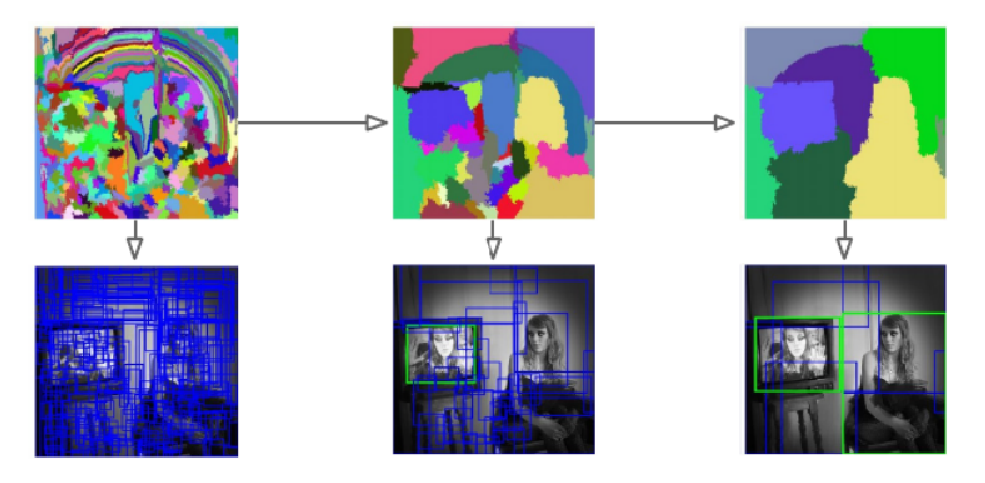
\includegraphics[scale=0.6]{pegado40}
\par\end{center}

\textbf{Intersection over Union (IoU)}

For two sets, $A$ and $B$, the Jaccard index, or Intersection over
Union, is the reatio of the intersection area to their union are
\[
J\left(A,B\right)=\frac{\left|A\cap B\right|}{\left|A\cup B\right|}.
\]

\textbf{Label region proposal}

Region proposal anchor boxes are associated to ground-truth bounding
boxes given their IoU (above a threshold). The class of an anchor
is the same as its associated bounding box. If the anchor box is not
associated to a bounding box, it is labeled as background.

The offsets, relative to the position of central coordinates between
anchor box and boundingbox, label the region.

That is, proposal anchor boxes are labeled with the same label of
a ground-truth bounding box if their IoU is above a given threshold.

\textbf{R-CNN}, by Girshick et al. in 2014

R-CNN takes region proposal as input. It computes features for each
of the regions, and the classification is done using several SVMs.
The regression of offsets is done by using a linear regression model.

To train R-CNNs, there is a supervised pretraining of a CNN backbone,
generally on ImageNet, followed by an optional fine-tuning of the
backbone, to learn specialised features based on a classification
obkective. The backbone is then fixed.

For each input: crop and wrap proposal regions computed by selective
search and compute the features. Train a binary SVM for each class,
and apply linear regression to crrect small offsets between the prediction
and the actual bounding box.
\begin{center}
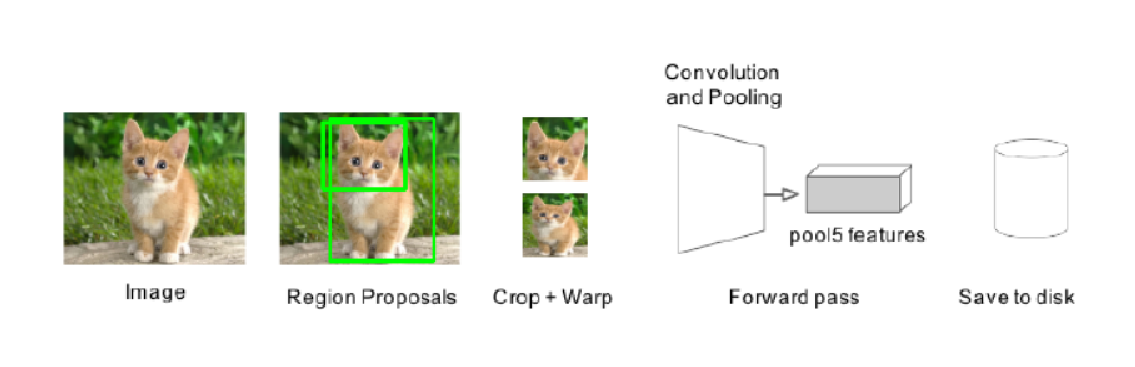
\includegraphics[scale=0.6]{pegado41}
\par\end{center}

\textbf{Evaluating detection models}

The meaning of true positive, false positive and false negative for
the detection problem is not the same as for regular classification
problems. The threshold for True and Falso positive/negatives is based
on the IoU and a given threshold. For example:
\begin{center}
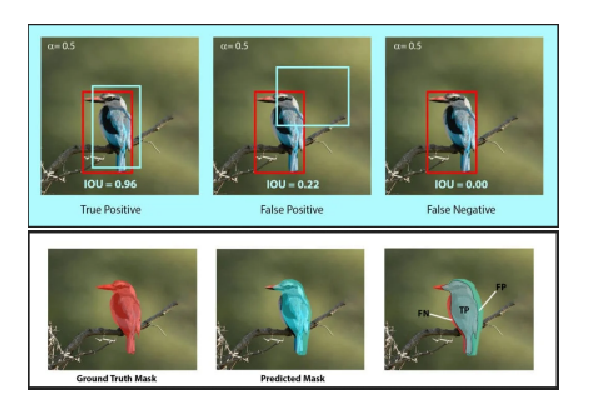
\includegraphics[scale=0.6]{pegado42}
\par\end{center}

Remember, $precision=\frac{TP}{TP+FP}$ and $recall=\frac{TP}{TP+FN}$.

The \textbf{average precision} is the area ander the prevision-recall
curve.

The \textbf{mean-average precision} is the mean of average precision
for various IoU threholds.

R-CNNs is slow in testing phase, because there are as many passes
in the CNN as the number of region proposals, which is around 2000.
Also, SVM and regression are a bit old school, so this architecture
is not usable for real world applications.

\textbf{Fast R-CNN}, by Girshick in 2015

This modification of R-CNN was proposed to increase its efficiency.
It passes thewhole image only once in the CNN backbone. The CNN is
trainable, and not fixed, and the proposed regions are associated
with computed features from the output feature map.

Each region of interest can have a different size, so selective search
proposed regions are concatenated with features from the CNN to form
the \textbf{Region of Interest (RoI) Pooling Layer}, which reshape
the features to feed them to fully connected layers. From these features
the classes and the offsets are predicted.

The following table compares R-CNN and Fast R-CNN:
\begin{center}
\begin{tabular}{|c|c|c|}
\hline 
 & R-CNN & Fast R-CNN\tabularnewline
\hline 
\hline 
Test time per image & 47 s & \textbf{0.32 s}\tabularnewline
\hline 
Speedup & 1x & \textbf{146x}\tabularnewline
\hline 
Test time per image with selective search & 50 s & \textbf{2 s}\tabularnewline
\hline 
Speedup & 1x & \textbf{25x}\tabularnewline
\hline 
\end{tabular}
\par\end{center}

\textbf{Faster R-CNN}, by Ren et al. in 2017

This new modification replaces selective search by a learned region
proposal network. The rest is similar to Fast R-CNN.

The \textbf{region proposal network (RPN)} is a network learned to
propose regions of interest. It slides a window on the feature size,
and, at each location of the window, it makes a prediction for $k$
anchors (propositions), which are sampled by varying scale and aspect
ratio. A small network predicts if there is an object there, and a
small network predicts offsets with the bounding box.

The following table compares the three approaches:
\begin{center}
\begin{tabular}{|c|c|c|c|}
\hline 
 & R-CNN & Fast R-CNN & Faster R-CNN\tabularnewline
\hline 
\hline 
Test time per image (with proposals) & 50 s & 2 s & \textbf{0.2 s}\tabularnewline
\hline 
Speedup & 1x & 25x & \textbf{250x}\tabularnewline
\hline 
mAP (VOC 2007) & 66.0 & \textbf{66.9} & \textbf{66.9}\tabularnewline
\hline 
\end{tabular}
\par\end{center}

\textbf{You Only Look Once (YOLO)}, by Redmon et al. in 2016

This model is a single stage detector: one network is used to predict
the bounding boxes and the class probabilities. It is the first real
time detector close to Faster R-CNN performance.

Its architecture consists of 24 convolutional layers and input dimension
of $448\times448$. For each input, it cuts it in $7\times7$ grids
of cells. Each cell computes the objectness and anchor boxes, considering
the object at the center of the cell, and enabling the boxes to reach
out the cell.

This model has been enhanced multiple times, with YoLo v2, v3, v4,
v5,...

\subsubsection{Semantic Segmentation}

The goal in this case is to find an object class for each pixel. There
are several associated problems:
\begin{itemize}
\item \textbf{Semantic segmentation}: associate each pixel to a specific
class.
\item \textbf{Instance segmentation}: associate each pixel to a specific
class and identify various instances from the same class.
\item \textbf{Panoptic segmentation}: associate each pixel to once class,
and prevent overlapping segments.
\end{itemize}
These are illustrated below:
\begin{center}
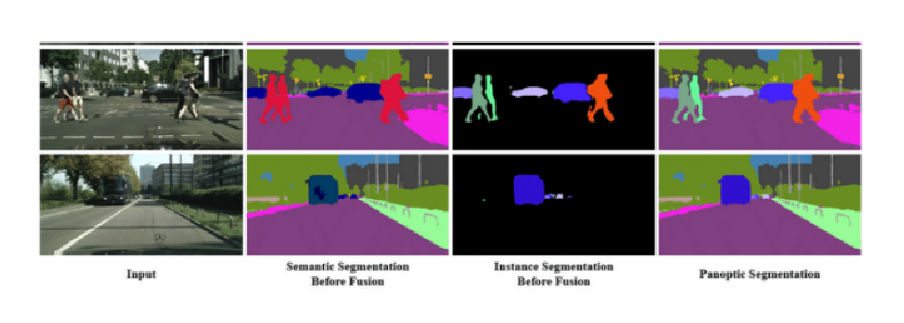
\includegraphics[scale=0.6]{pegado43}
\par\end{center}

\textbf{Mask R-CNN} by He et al. in 2017

Basically, it is Faster R-CNN with a third branch, which outputs the
object mask. 

It can use various backbones such as ResNet, DenseNet,...

\subsection{Data and Transfer}

Modern CNNs are made of millions of parameters, requiring a huge amount
of data to train them. For example, ImageNet has 1.2M images for 1k
classes, and is being replaced by ImageNet21k, that has 1B images.

Manually annotating such amount of images is costly in terms of money
and time, and therefore there is the need for techniques to deal with
lacking of data: data augmentation and transfer learning.

\subsubsection{Data Augmentation}

We already saw it! It increases the diversity of data by transforming
the source data with invariants

\subsubsection{Transfer Learning}

Sometimes there is possibility to learn from scratch, by random initialisation,
because of lack of data. In this case, we can make use of an already
\textbf{pre-trained} backbone from a source task for the target task.
\begin{itemize}
\item If the target task is similar to the source task, and the size is
comparable, transfer learning works directly; while if the size is
inferior, there is a risk of overfitting to the target task after
few epochs.

For small problems, the transfer learning is accomplished by learning
a linear classifier with last layers of a pre-trained backbone.
\item If the target task is very different from the the source task, and
the problem is small, a linear classifier from lower level layers
can be used; if the problem is large, we can fine-tune the backbone
to the new task.
\end{itemize}
In all cases, starting from initialized weights is better than nothing.

\textbf{Fine tuning}

Fine tuning consists in training several layers of a pre-trained backbone:
\begin{center}
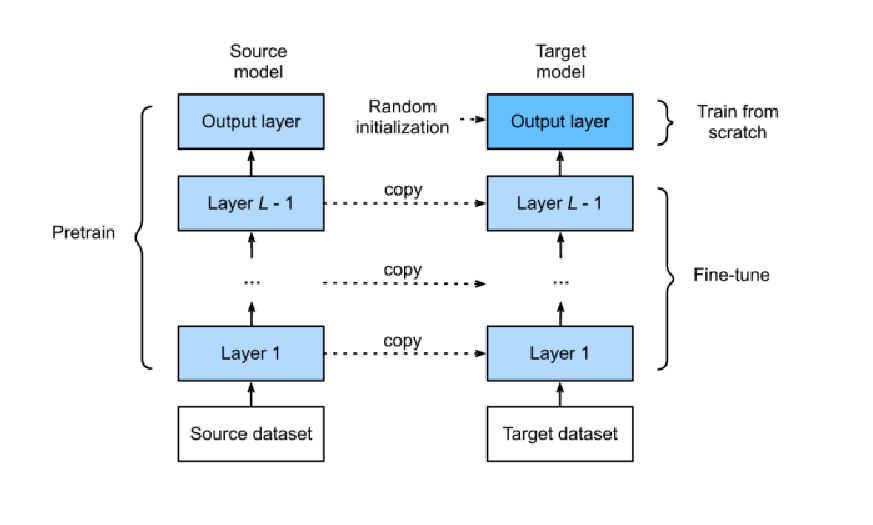
\includegraphics[scale=0.6]{pegado44}
\par\end{center}

\textbf{Domain Adaptation}

Sometimes, the target task and the source task share the same classes,
but the target data has a different distribution than the source.
This is an entire field in ML: how to adapt our features to the new
domain, and have the best possible results.

\subsection{Self-Supervised Learning (SSL)}

We already know supervised learning. It consists on predicting a target
associated to an input. 

Self-Supervised Learning (SSL) is different. It consists on predicting
a part of en input, from the input. This means the model learns to
understand and generate data by teaching itself.

A \textbf{pretext task} is a task designed to teach the model something
about the structure of the input data without using labels. For example,
the pretext task might involve predicting the next word in a sentence,
or the color version of a grayscale image. The idea is to construct
targets from the data itself and learn from these artificially created
labels.

SSL presents several advantages:
\begin{itemize}
\item Reduces the Need for Labeled Data: Labeling is often expensive and
time-consuming, and SSL offers a way to learn useful representations
without the need for extensive labeled datasets. 
\item Better Pre-training: SSL can serve as pre-training for neural networks,
allowing them to learn general features from the data that can then
be refined with a smaller amount of labeled data for a specific task
(using transfer learning).
\end{itemize}
All this is illustrated below:
\begin{center}
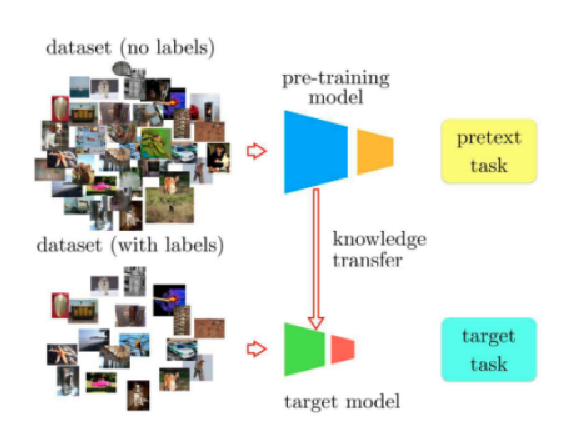
\includegraphics[scale=0.6]{pegado45}
\par\end{center}

For images, several pretext tasks have been firstly proposed, like
rotation, patch localization, colorization, counting,...

For videos, which add the time dimension, we find the same pretext
tasks as in images, plus some others specific to videos, which can
be masking frames, shuffling frames,...

\textbf{Contrastive Learning}

Constrastive Learning is a pretext task for SSL. It aligns positively
pairs of images, and push away other images. We find the problem of
defining what is a positive pair, which can be solved by using data
augmentation.

The following figure illustrates this concept:
\begin{center}
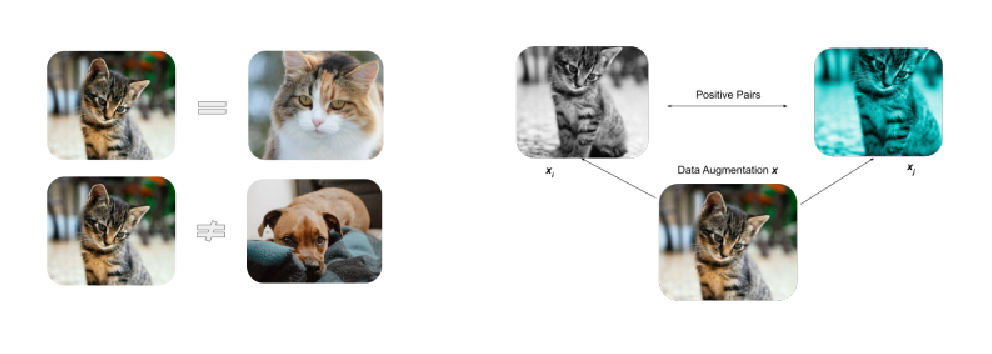
\includegraphics[scale=0.6]{pegado46}
\par\end{center}

\textbf{SimCLR}, by Chen et al. in 2020

This model defines a siamese pipeline for contrastive learning. Positive
pairs are formed from strong data augmentation, like color jittering,
gaussian blur, grayscale, etc. Both paris go through an encoder and
a projector, which consists on several stacked MLP layers. Then, contrastive
loss is applied.
\begin{center}
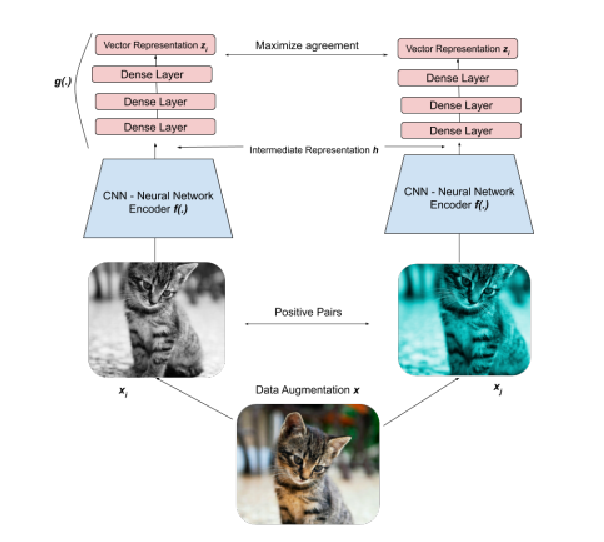
\includegraphics[scale=0.6]{pegado47}
\par\end{center}

\textbf{SCE}, by Denize et al. in 2021

This model tries to address the problem of how to deal with negatives
that share semantic information with the positive pairs. For example,
two different cats share more information than two different dogs.
Pushing negatives with high semantic similarities makes training unstable,
and so SCE predicts positive pairs and estimated relations among instances.

\textbf{Deep Cluster}, by Caron et al. in 2018

Clustering associates several input data to a same pseudo-label, without
supervision.

Deep Cluster applies clustering to traing a backbone using several
stages:
\begin{itemize}
\item Estimate pseudo-labels for each instance with a fixed backbone.
\item Train the backbone on this label.
\item Repeat the operations until convergence.
\end{itemize}

\section{Recurrent Neural Networks}

\subsection{Introduction}

Recurrent Neural Networks are a family of Neural Network architectures
specially designed to deal with sequential data, such as text in NLP,
speech signals in speech2text tasks, temporal data in videos, or other
temporal signals, like ECGs, time series, etc.

\textbf{Sequential data} is data with a temporal component, that usually
implies correlation in the temporal dimension. More precisely, a \textbf{sequence}
consists in a set of vectors $x_{t}$, where $t\in\left[1,\tau\right]$
is a temporal index.

Note that the temporal index is not necessarily related to time, but
to order. For example, text is not temporal, but words are ordered.

\textbf{Memory} is essential for us to understand and interpret what
we perceive. Memory can be understood as a persistent format of information.
MLP don't have this persistence, each data point is processed independently
of the rest. Therefore, RNNs introduce a way to store information,
by adding inner loops that enables them to preserve information at
each time-step.

\subsection{Recurrent Neural Networks}

A Recurrent Neural Network (RNN) is defined with a state, $h^{\left(t\right)}$,
by recurrence. This state depends on the current input, $x^{\left(t\right)}$,
and the previous state, $h^{\left(t-1\right)}$:
\[
h^{\left(t\right)}=f\left(h^{\left(t-1\right)},x^{\left(t\right)};\theta\right).
\]
 The computational graph can be represented with a loop, or unfolded,
making it direct and acyclic, as:
\begin{center}
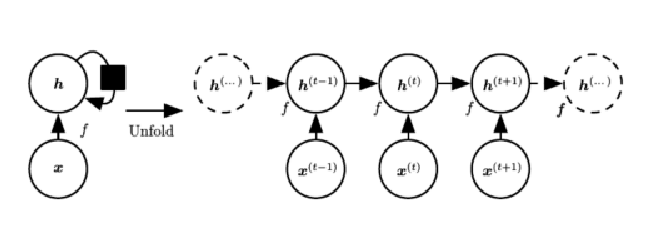
\includegraphics[scale=0.6]{pegado50}
\par\end{center}

A RNN is trained to predict the future, given past information, in
such a way that $h^{\left(t\right)}$ is a summary of the sequence
until the timestep $t$. This summarization implies information compression,
or loss of information, and the training must keep relevant information
for the task.

Going back to the definition of the state, we can then write it alternative
as
\[
h^{\left(t\right)}=f\left(h^{\left(t-1\right)},x^{\left(t\right)};\theta\right)=g^{\left(t\right)}\left(x^{\left(t\right)},x^{\left(t-1\right)},...,x^{\left(1\right)}\right),
\]
 where $g^{\left(t\right)}$ takes the whole sequence as input, of
variable length.

On the other hand, using the factorized form, with \textbf{transition
function $f$}, the function is the same at each timestep, allowing
for parameter sharing and generalization.

\begin{tcolorbox}
\begin{thm}
RNNs are universal approximators.
\end{thm}
\end{tcolorbox}

We measure the performance of a RNN through the cost function $L$,
between the output $o$ and the ground truth $y$. Internatlly, we
use softmax:
\[
\hat{y}_{i}=\frac{e^{o_{i}}}{\sum_{j}e^{o_{j}}}.
\]
 The parameters of a RNN are:
\begin{itemize}
\item $U$: input to hidden layers.
\item $W$: recurrent connections between hidden layers.
\item $V$: hidden layers to output.
\end{itemize}
That is:
\begin{center}
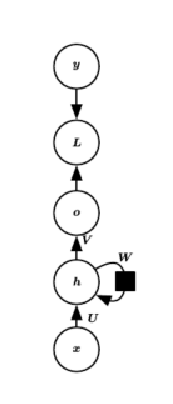
\includegraphics[scale=0.6]{pegado51}
\par\end{center}

\subsubsection{Direct Propagation}

In the case of discrete variable prediction (like words), $o$ represents
log-likelihoods of possible output values, and the normalize probability
is $\hat{y}=softmax\left(o\right)$.

Direct propagation works by:
\begin{align*}
a^{\left(t\right)} & =b+Wh^{\left(t-1\right)}+Ux^{\left(t\right)},\\
h^{\left(t\right)} & =\phi\left(a^{\left(t\right)}\right),\\
o^{\left(t\right)} & =c+Vh^{\left(t\right)},\\
\hat{y}^{\left(t\right)} & =softmax\left(o^{\left(t\right)}\right),
\end{align*}
 where $\phi$ is the activation function.

\subsubsection{Recurrent Neural Networks with output recurrence}

We don't link directly hidden layers recurrently, but rather we link
the output to a hidden layer. This has the cons of using less information
than $h^{\left(t-1\right)}$, being therefore a less expressive model,
but the pros of being easier to train, enabling parallelization and
efficient backpropagation.
\begin{center}
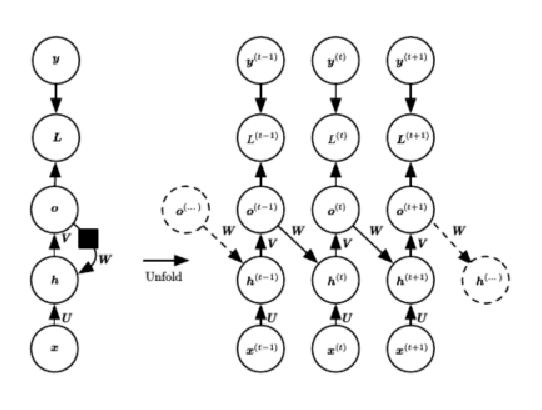
\includegraphics[scale=0.6]{pegado52}
\par\end{center}

\subsubsection{Recurrent Neural Networks with unique output}

In this case, it needs the complete input sequence, and the output
is a summary of the input. This kind of setting is usually used a
simpler module of a more complex architecture.
\begin{center}
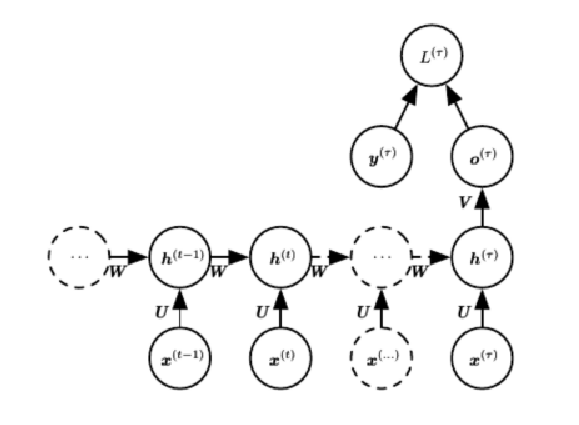
\includegraphics[scale=0.6]{pegado53}
\par\end{center}

\subsubsection{More architectures}

In this figure we observe different possible setups, which apply to
different use cases.
\begin{center}
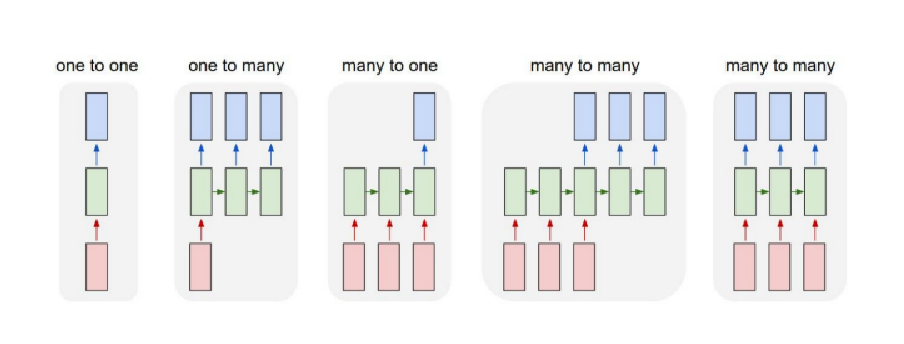
\includegraphics[scale=0.6]{pegado54}
\par\end{center}

For instance:
\begin{itemize}
\item Automatic captioning, converting images to text sequences, could be
done with a one to many architecture.
\item Sentiment analysis, converting a text sequence to a predicted label,
could be done with a many to one architecture.
\item Machine translation, converting text sequence to text sequence, could
be done with a many to many architecture.
\item Frame-label video classification, converting a video sequence into
a sequence of labels, could also be done with a many to many architecture.
\end{itemize}

\subsubsection{Bi-Directional Recurrent Neural Network}

Sometimes, the future of the sequence can also be helpful, for example
in NLP, in Character recognition and even in Speech recognition. For
this, there exist the Bi-Directional RNN (BRNN), which combine a RNN
processing from past to future, with state $h$, and a RNN processing
from future to past, with state $g$, and the output combines the
two of them.
\begin{center}
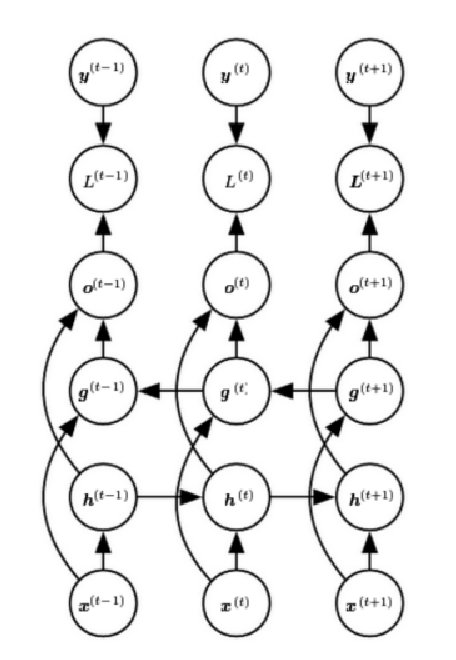
\includegraphics[scale=0.6]{pegado55}
\par\end{center}

Moreover, BRNN can be applied to images with 4 direction, applying
them up,down and left,right. This is a bit outdated approach for visual
recognition, with architectures as ReNet for classification and ReSeg
for segmentation.

\subsubsection{Deep Recurrent Neural Network}

A classical RNN has an input layer, $U$, a hidden layer, $W$, and
an output layer $V$. However, we can add hidden layers, allowing
to go higher in abstraction.

The representation improves hierarchically:
\begin{itemize}
\item $h$, the first state, represents temporal dependencies on inputs
$x$.
\item $z$, the second state, represents temporal dependencies on the representations
$h$.
\end{itemize}
\begin{center}
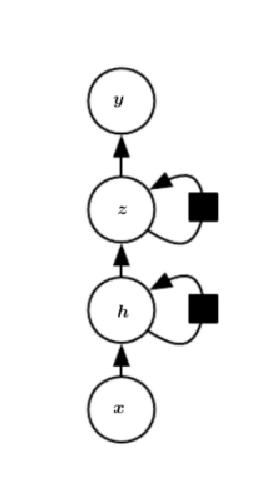
\includegraphics[scale=0.6]{pegado56}
\par\end{center}

Also, we can add an MLP before every recurrent layer, increasing the
representation capacity of the network, at the expense of a harder
training. A possibility to improve these is to use skip connections.

\subsection{Recurrent Neural Networks Training}

The principle is the same as with MLP and CNNs: we choose a cost function
a minimize it during training using gradient descent with backpropagation.

However, we need to take into account the recurrency of the network,
and so we use what is called \textbf{Backpropagation through time
}(BPTT), which consists in applying backpropagation to an unrolled
graph of the RNN.

The idea is to forward through the entire sequence to compute the
loss, and then go backwards through the entire sequence to compute
gradient.

However, this can be very inefficient, so we also find the \textbf{truncated
BPTT}, which does BPTT to chunks of the sequence, instead of the complete
sequence. The hidden states are carried forward in time until the
end of the sequence, but we only backpropagation for some smaller
number of steps.
\begin{center}
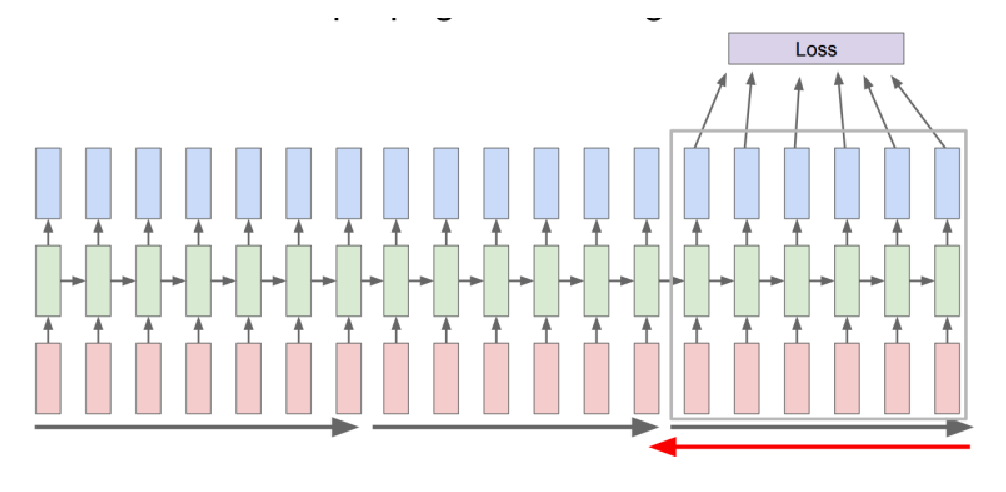
\includegraphics[scale=0.5]{pegado57}
\par\end{center}

\subsection{Long-Short Term Memory (LSTM) and Gated Recurrent Units (GRU)}

Classical RNN present two main limitations:
\begin{enumerate}
\item A computation limitation: they are hard to train, and prone to gradient
vanishing and explosion.
\item Long term interactions are hard to model.
\end{enumerate}
Some upgraded variants of RNNs are Long Short Term Memory (LSTM) and
Gated Recurrent Units (GRU).

\textbf{Gradient vanishing and exploding}: the reason RNNs are prone
to gradient vanishing/exploding is that the gradient needs to go through
the unfolded computational graph. If the largest singular value of
the hidden matrix is greater than 1, a recurrent multiplication by
it would tend to increase the gradient vector, leading to gradient
explosion. The opposite happens when the largest singular value is
smaller than 1, leading to gradient vanishing.

The solution to gradient explosion can be using gradient clipping.

The solution to gradient vanishing is to change the RNN architecture.

\textbf{Long-term dependency problem}: RNNs can connect past information
to present data, and, in theory, time distance of information is irrelevant.
However, in practice, classical RNNs cannot model long sequences (more
than 20 points).

\subsubsection{LSTM}

LSTM is based on a standard RNN whose neuron activates with $tanh$.
\begin{center}
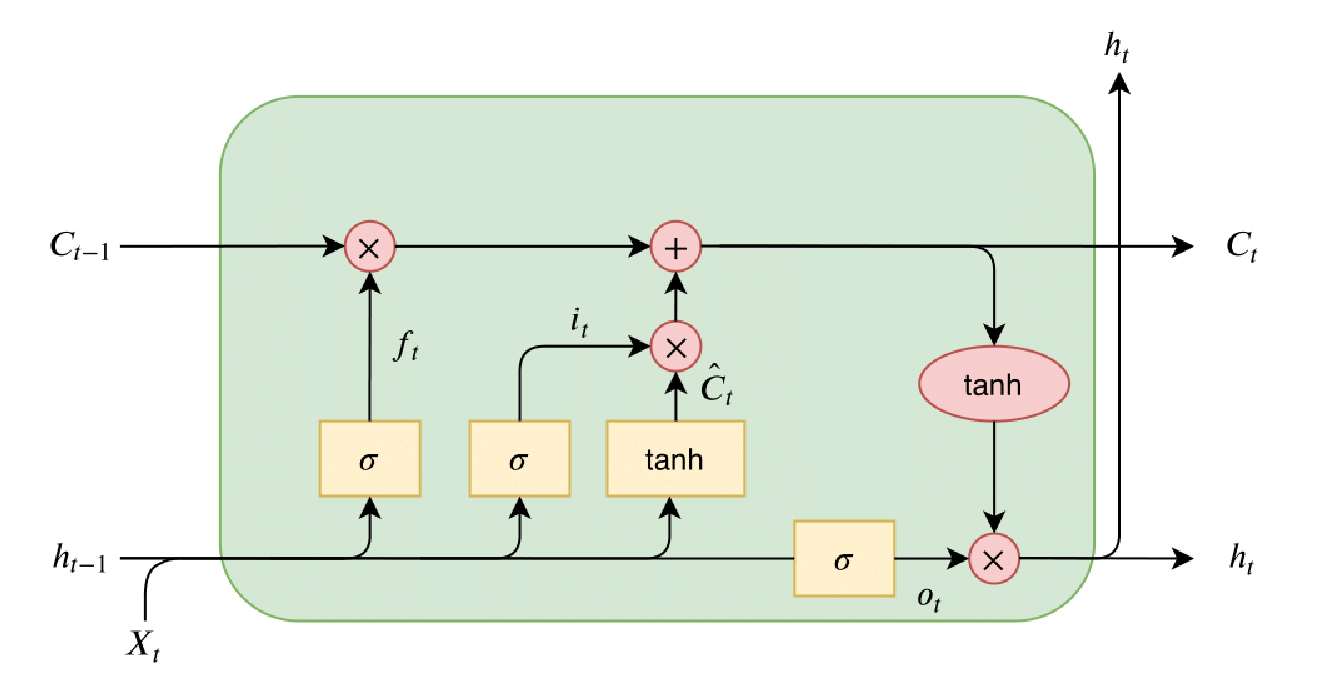
\includegraphics[scale=0.5]{pegado58}
\par\end{center}

$C_{t}$ is the cell state, which flows through the entire chain and
is updated with a sum instead of a product. This avoids memory vanishing
and the gradient explosion and vanish. 

Then, there are three gates foverned by sigmoid units, which define
the control of in and out information.

A key component is the forget gate,
\[
f_{t}=\sigma\left(W_{f}\cdot\left[h_{t-1},x_{t}\right]+b_{f}\right),
\]
 which can affect the affect the previous state, letting it through
or not (forgetting).

Then, the input gate layer,
\[
i_{t}=\sigma\left(W_{i}\cdot\left[h_{t-1},x_{t}\right]+b_{i}\right),
\]
 which processes the input, contributing to the cell state.

Then, there is the classical neuron, activated with $tanh$, which
also contributes to the cell state, by
\[
\hat{C}_{t}=tanh\left(W_{C}\cdot\left[h_{t-1},x_{t}\right]+b_{C}\right).
\]

Finally, to update the cell state it is
\[
C_{t}=f_{t}\cdot C_{t-1}+i_{t}\cdot\hat{C}_{t}.
\]
 Notice that the output is computed as
\[
h_{t}=tanh\left(C_{t}\right)+\sigma\left(W_{o}\cdot\left[h_{t-1},x_{t}\right]+b_{o}\right).
\]


\subsubsection{GRU}

GRU is a variant of LSTM, simpler and faster, and with similar performance.
It works by applying:
\begin{align*}
u_{i} & =\sigma\left(W_{u}\cdot x_{i}+U_{u}\cdot h_{i-1}+b_{u}\right),\\
r_{i} & =\sigma\left(W_{r}\cdot x_{i}+U_{r}\cdot h_{i-1}+b_{r}\right),\\
\hat{h}_{i} & =tanh\left(W_{h}\cdot x_{i}+r_{i}\circ U_{h}\cdot h_{i-1}+b_{h}\right),\\
h_{i} & =u_{i}\circ\hat{h}_{i}+\left(1-u_{i}\right)\circ h_{i-1}.
\end{align*}

\begin{center}
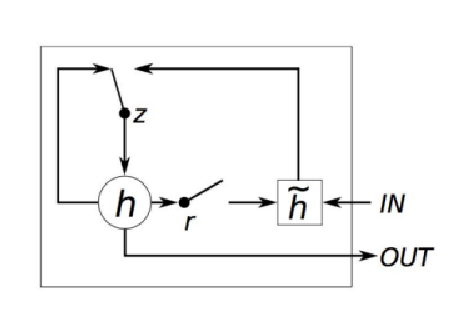
\includegraphics[scale=0.6]{pegado59}
\par\end{center}

Even with these improvements, RNN struggle with long sequences, and
remain difficult and slow to train, because of thei autoregressive
nature. In 2017, a Google paper introduced a novel architecture that
changed everything: the Transformer.

\section{Deep Generative Modelling}

Recall that the objective of supervised learning is to learn a mapping,
$f$, between a data sample, $x$, and its label, $y$:
\[
y=f\left(x\right).
\]
 This can be formalized by learning the conditional distribution between
labels, given a data point, that is, $p\left(y|x\right)$.

For this task, we need to have access the annotated pairs $\left(x,y\right)$.
The applications of supervised learning are classification, object
detection, segmentation, etc.

On the other hand, unsupervised learning tries to learn the underlying
hidden data structure, formalized by the unconditional distribution
data points, $p\left(x\right)$. 

In this case, we don't need any annotations to the data. The applications
of unsupervised learning are generative modelling, clustering, feature
learning, summarization, etc.

\textbf{Generative modelling} consists in learning a model, $M$,
that can approximate the data distribution, 
\[
p_{M}\left(x\right)\sim p\left(x\right),
\]
 and should enable sampling easily. That is, a generative model aims
to provide:
\begin{itemize}
\item Density estimation: it can evaluate the likelihood of a data point
belonging to the original distribution.
\item Sampling: it can provide likely samples.
\end{itemize}

\subsection{Variational Auto-Encoders (VAE)}

\subsubsection{Auto-Encoders}

AEs are a type of unsupervised model used to learn low-dimensional
latent representations, $z$, of data samples, $x$. This means that
the aim is to somehow try to summarize the input data space, $X$,
into a smaller space, $Z$, so $dim\left(Z\right)<dim\left(X\right)$.
$Z$ should capture relevant characteristics of data, and the choice
of its dimensionality is a compromise between interpretability and
the amount of information to keep.

In Figure \ref{fig:Illustration-of-autoencoders.} we can see an illustration
of autoencoders. The input is processed by the encoder, which is able
to embed it into a smaller space, the \textbf{latent space}. The decoder
can take the point in the latent space and reconstruct the original
image.

To train them, this process is applied to the training set, and the
loss function is the distance between the reconstructed images and
the original ones:
\[
\mathcal{L}\left(M,X\right)=\sum_{x\in X}\left\Vert M\left(x\right)-x\right\Vert ^{2}.
\]

\begin{figure}
\begin{centering}
\includegraphics[scale=0.1]{autoencoder}
\par\end{centering}
\caption{\label{fig:Illustration-of-autoencoders.}Illustration of autoencoders.
Source: \protect\url{https://www.v7labs.com/blog/autoencoders-guide}.}
\end{figure}

The \textcolor{red}{problem} of AEs is that they don't allow generation,
because the distribution of $p\left(z\right)$ is difficult to sample
from.

To see this more clearly, let's discuss an example done by Joseph
Rocca, \href{https://towardsdatascience.com/understanding-variational-autoencoders-vaes-f70510919f73}{Understanding VAEs}.

In the following image, we observe how, when using AEs, points in
the latent space can have no real meaning, making it difficult to
sample and generate new objects, which is the ultimate goal of generative
models.
\begin{center}
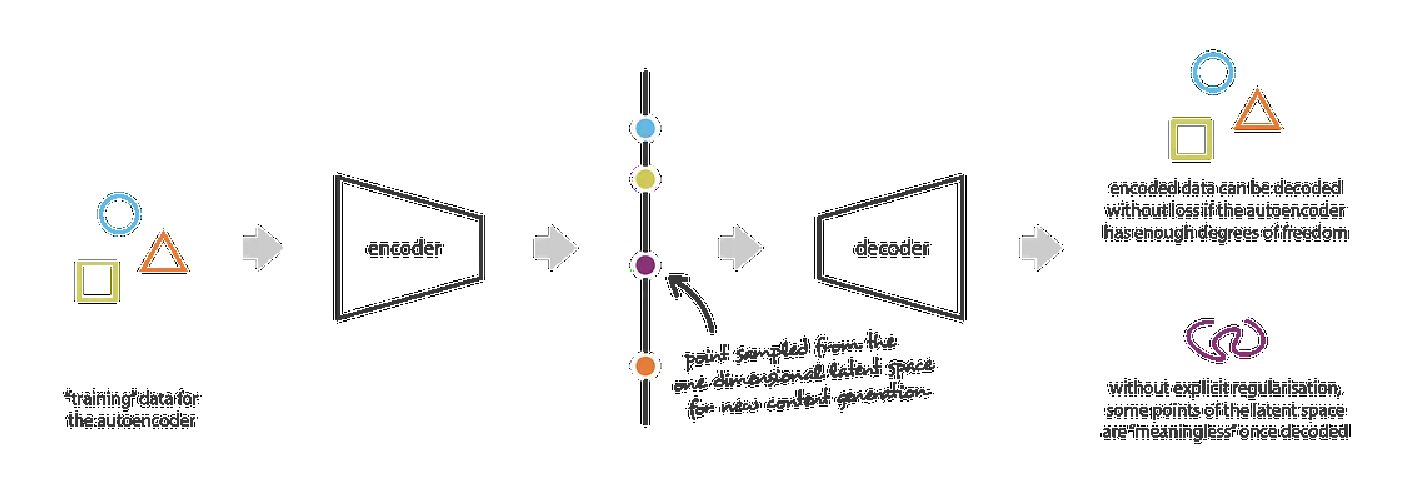
\includegraphics[scale=0.6]{pegado60}
\par\end{center}

What is desirable, is that somehow, points in the latent space that
are close to each other, should have a similar real meaning, once
they are decoded:
\begin{center}
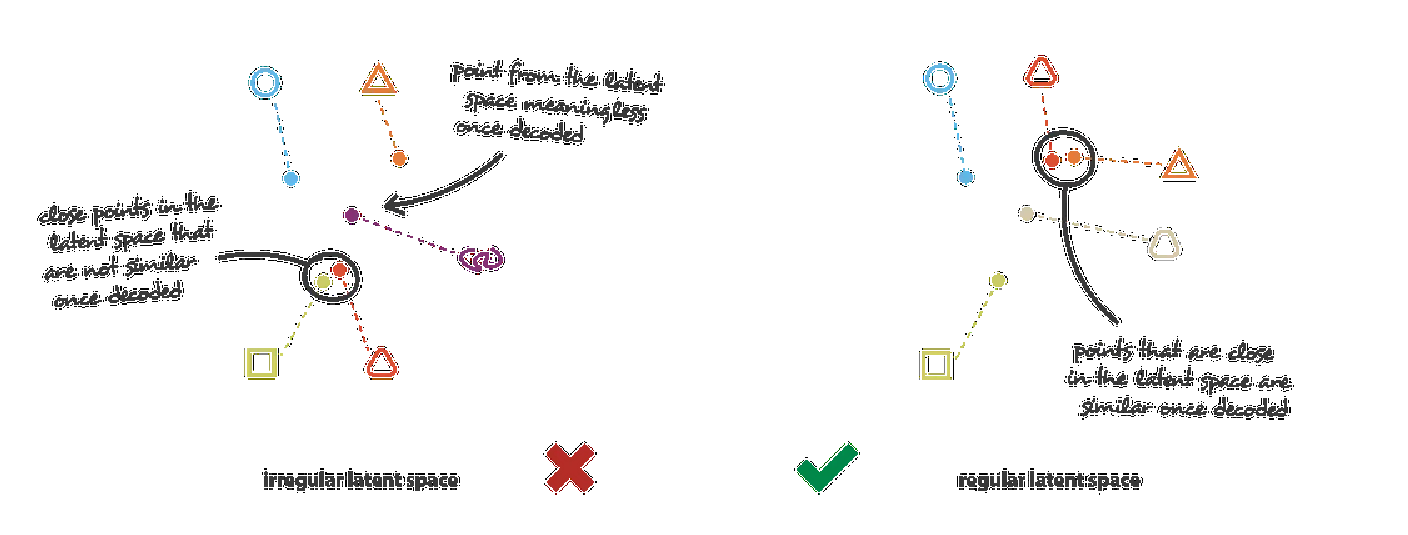
\includegraphics[scale=0.6]{pegado61}
\par\end{center}

This cannot be achieved with AEs, and this led to the introduction
of Variational Auto-Encoders (VAEs).

\subsubsection{Variational Auto-Encodersi}

In this case, the latent representation is not directly learnt, but
rather a \textbf{latent distribution}. In Figure \ref{fig:Illustration-of-a},
we observe the illustration of VAEs.

\begin{figure}
\begin{centering}
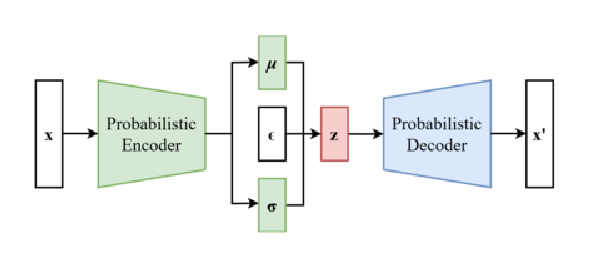
\includegraphics{pegado62}
\par\end{centering}
\caption{Illustration of a variational auto-encoder.\label{fig:Illustration-of-a}.
Source: \protect\href{https://en.wikipedia.org/wiki/Variational_autoencoder}{Wikipedia}.}
\end{figure}

In this case, training is more complex. We want to mazimize the data
likelihood. More precisely, its log-likelihood:
\[
\mathcal{L}\left(\theta,\phi,x\right)=\log p_{\theta}\left(x\right).
\]
 Notice that this is not dependent on the distribution of $z$, $q_{\phi}$,
so we can write:
\[
\log p_{\theta}\left(x\right)=\mathbb{E}_{z\sim q_{\phi}\left(z|x\right)}\left[\log p_{\theta}\left(x\right)\right],
\]
 and applying the reversed Bayes' Rule:
\[
\mathbb{E}_{z}\left[\log p_{\theta}\left(x\right)\right]=\mathbb{E}_{z}\left[log\frac{p_{\theta}\left(x|z\right)p_{\theta}\left(x\right)}{p_{\theta}\left(z|x\right)}\right].
\]
 Here, we can multiply and divide by $q_{\phi}\left(z|x\right)$ and
use the properties of logarithms, to get:
\[
\mathbb{E}_{z}\left[\log p_{\theta}\left(x\right)\right]=\mathbb{E}_{z}\left[\log p_{\theta}\left(x|z\right)\right]-\mathbb{E}_{z}\left[\log\frac{q_{\phi}\left(z|x\right)}{p_{\theta}\left(z\right)}\right]+\mathbb{E}_{z}\left[\log\frac{q_{\phi}\left(z|x\right)}{p_{\theta}\left(z|x\right)}\right].
\]
 Now, recalling the definition of the Kullback-Leibler Divergence:
\[
D_{KL}\left(P\parallel Q\right)=\mathbb{E}_{P}\left[\log\frac{P\left(x\right)}{Q\left(x\right)}\right],
\]
 we can rewrite:
\[
\mathcal{L}\left(\theta,\phi,x\right)=\mathbb{E}_{z}\left[\log p_{\theta}\left(x|z\right)\right]-D_{KL}\left(q_{\phi}\left(z|x\right)\parallel p_{\theta}\left(z\right)\right)+D_{KL}\left(q_{\phi}\left(z|x\right)\parallel p_{\theta}\left(z|x\right)\right).
\]
 Now, the last term is very difficult to compute, because $p_{\theta}\left(z|x\right)$
is intractable. Since it is bigger than 0, we can bound $\mathcal{L}$
from below by
\[
\mathcal{L}\left(\theta,\phi,x\right)\geq\mathbb{E}_{z}\left[\log p_{\theta}\left(x|z\right)\right]-D_{KL}\left(q_{\phi}\left(z|x\right)\parallel p_{\theta}\left(z\right)\right),
\]
 this is called the \textbf{Evidence Lower Bound}. The first term
is called the \textbf{reconstruction term}, and can be approximated
by sampling and serves to ensure good reconstructions of the output.
The second term is the \textbf{regularisation term}, which makes the
distribution of the encoder close to the prior.

The impact of the regularisation is that it enables for \textbf{continuity}
in the latent representation, so that similar data samples have similar
latent representations; and it helps to ensure \textbf{completeness}
of the latent space, so that all latent points have a meaningful decoding.

Joseph Rocca illustrates this as:
\begin{center}
\includegraphics[scale=0.6]{pegado63}
\par\end{center}

In addition to enabling continuity and completeness, or maybe thanks
to this, VAEs enable a much easier sampling and generation. We can
just sample $z$ from a normal distribution, and process it through
the decoder.

\subsection{Generative Adversarial Networks}

Now, the objective is to sample for a high dimensional and multi-modal
distribution, $p\left(x\right)$, by learning a mapping, $G$, between
a simple distribution from which we can sample and the high dimensional
distribution. For this, Generative Adversarial Networks (GANs), consist
of two components:
\begin{itemize}
\item \textbf{Discriminator}: tries to distinguish between generated and
real data.
\item \textbf{Generator}: tries to fool the discriminator by creating likely
samples.
\end{itemize}
This is illustrated below:
\begin{center}
\includegraphics[scale=0.6]{pegado64}
\par\end{center}

To train these models, we follow a minimax approach: the discriminator
aims at maximizing its success rate, while the generator aims to minimizing
the success rate of the discriminator. This can be expressed as:
\begin{align*}
\mathcal{J}\left(D,G,X\right) & =\min_{G}\max_{D}V\left(D,G,X\right)\\
 & =\min_{G}\max_{D}\mathbb{E}_{x\sim p_{data}\left(x\right)}\left[\log D\left(x\right)\right]+\mathbb{E}_{z\sim p_{z}\left(z\right)}\left[\log\left(1-D\left(G\left(z\right)\right)\right)\right].
\end{align*}
 This can be divided:
\begin{itemize}
\item The \textbf{discriminator loss} is
\[
\mathcal{J}\left(D,X\right)=\max_{D}\mathbb{E}_{x\sim p_{data}\left(x\right)}\left[\log D\left(x\right)\right]+\mathbb{E}_{z\sim p_{z}\left(z\right)}\left[\log\left(1-D\left(G\left(z\right)\right)\right)\right].
\]
\item The \textbf{generator loss} is
\[
\mathcal{J}\left(G,X\right)=\min_{G}\mathbb{E}_{z\sim p_{z}\left(z\right)}\left[\log\left(1-D\left(G\left(z\right)\right)\right)\right].
\]
 
\end{itemize}
Once the training is done, generation is quite straightforward. We
only need to sample $z\sim p_{z}\left(z\right)$ and process it with
the generator module.

An interesting property of GANs is that they show continuous representations
of the latent space, as shown in the figure below:

\begin{figure}
\begin{centering}
\includegraphics[scale=0.6]{pegado65}
\par\end{centering}
\caption{Interpolating in the latent space of GANs. Source: \cite{radford2015}.}
\end{figure}

In the following table, we compare GANs and VAEs in different aspects:
\begin{center}
\begin{tabular}{|c|c|c|c|c|c|}
\hline 
 & Sample Quality & Inference & Mode Coverage & Training Quality Assesment & Training Stability\tabularnewline
\hline 
\hline 
VAE & Intermediate & Good & Good & Good & Good\tabularnewline
\hline 
GAN & Very good & Bad & Intermediate & Intermediate & Intermediate\tabularnewline
\hline 
\end{tabular}
\par\end{center}

\subsection{Other Approaches}

\subsubsection{Normalizing Flows}

The idea is to transform a simple distribution into acomplex one,
by applying a sequence of invertible transformation functions.

The pros of this approach is that it provides good sample quality,
exact inference and stable training. However, it requires invertible
neural networks.

\subsubsection{Pixel RNN}

This approach consists in generated image pixels starting from the
corner. The dependencies between the current pixel and the previous
ones is modelled using an RNN. The biggest drawback of this approach
is that sequential generation is very slow.

\section{Denoising Diffusion Models}

To train diffusion models, there are two processes involved:
\begin{itemize}
\item Forward process: gradually adds noice to the input, until obtaining
a completely noisy image.
\item Reverse process: learns to generate data by denoising.
\end{itemize}
This is illustrated in this Figure:
\begin{center}
\includegraphics[scale=0.6]{pegado66}
\par\end{center}

The forward process can be seen as a Markov process, with starting
state $x_{0}$ and transition probability $q\left(x_{t}|x_{t-1}\right)$
for $t=1,...,T$:
\[
x_{0}\overset{q\left(x_{1}|x_{0}\right)}{\rightarrow}x_{1}\overset{q\left(x_{2}|x_{1}\right)}{\rightarrow}x_{2}\overset{q\left(x_{3}|x_{2}\right)}{\rightarrow}...\overset{q\left(x_{T-1}|x_{T-2}\right)}{\rightarrow}x_{T-1}\overset{q\left(x_{T}|x_{T-1}\right)}{\rightarrow}x_{T}
\]
 The transition probability or \textbf{Markov kernel} is usually chosen
to be
\[
q\left(x_{t}|x_{t-1}\right)=\mathcal{N}\left(x_{t};\sqrt{1-\beta_{t}}x_{t-1},\beta_{t}I\right),\ \beta_{t}\in\left(0,1\right),
\]
 but it can be any Markov Diffusion Kernel. The property of these
kernels is that they converge to a standard distribution. In this
case, they converge to a normal distribution, always the same, no
matter the input, $x_{0}$.

Thus, the forward trajectory can be expressed as
\[
q\left(x_{0;T}\right)=q\left(x_{0}\right)\prod_{t=1}^{T}q\left(x_{t}|x_{t-1}\right).
\]
 And to go to step $t$, from the step $t-1$, we just need to sample
from the kernel distribution.

It is also possible to go advance several steps at once. For this,
we can define the parameters:
\[
\begin{cases}
\alpha_{t}=1-\beta_{t}\\
\hat{\alpha}_{t}=\prod_{s=1}^{t}\alpha_{s}
\end{cases},
\]
 and use the Markov kernel
\[
q\left(x_{t}|x_{0}\right)=\mathcal{N}\left(x_{t};\sqrt{\hat{\alpha}_{t}}x_{0},\left(1-\hat{\alpha}_{t}\right)I\right),
\]
 which is equivalent to do
\[
x_{t}=\sqrt{\hat{\alpha}_{t}}x_{0}+\sqrt{1-\hat{\alpha}_{t}}\varepsilon
\]
 with $\varepsilon\sim\mathcal{N}\left(0,I\right)$. This allows to
go to any node in the chain in just one step.

The parameter $\beta_{t}$ is the \textbf{noise scheduler}, and it's
chosen to have increasing variance, in such a way that $q\left(x_{T}\right)$
is a standard Gaussian. If the $\beta_{t}$-s are small enough, the
reverse transitions are also Gaussian, but $q\left(x_{t-1}|x_{t}\right)$
in intractable, but using the Bayes rule we know that
\[
q\left(x_{t-1}|x_{t}\right)\propto q\left(x_{t-1}\right)q\left(x_{t}|x_{t-1}\right),
\]
 and we can use a model to approximate this reverse process.

That is, we are going to train a model to approximate the reverse,
denoising, process. This parametric reverse model:
\begin{itemize}
\item Is also a Markov chain, starting at $x_{T}$.
\item It starts with $p\left(x_{T}\right)=\mathcal{N}\left(x_{T};0,I\right)$,
since $q\left(x_{T}\right)\approx\mathcal{N}\left(0,I\right)$.
\item Its transitions are learned.
\end{itemize}
So, how may we achieve this? 

The reverse process is:
\[
x_{0}\overset{p_{\theta}\left(x_{0}|x_{1}\right)}{\leftarrow}x_{1}\overset{p_{\theta}\left(x_{1}|x_{2}\right)}{\leftarrow}x_{2}\overset{p_{\theta}\left(x_{2}|x_{3}\right)}{\leftarrow}...\overset{p_{\theta}\left(x_{T-2}|x_{T-1}\right)}{\leftarrow}x_{T-1}\overset{p_{\theta}\left(x_{T-1}|x_{T}\right)}{\leftarrow}x_{T}
\]
 So the reverse transitions are
\[
p_{\theta}\left(x_{t-1}|x_{t}\right)=\mathcal{N}\left(x_{t-1};{\color{red}\mu_{\theta}\left(x_{t},t\right)},\sigma_{t}^{2}I\right),
\]
 and $\mu_{\theta}\left(x_{t},t\right)$ will be our trainable network!
The reverse trajectory is then
\[
p_{\theta}\left(x_{0;T}\right)=p\left(x_{T}\right)\prod_{t=1}^{T}p_{\theta}\left(x_{t-1}|x_{t}\right).
\]
 To train this, we follow a maximum likelihood approach:
\[
\mathcal{J}\left(x,\theta\right)=-\log p_{\theta}\left(x_{0}\right)
\]
 Now, we can marginalize by integrating over the latents:
\[
-\log p_{\theta}\left(x_{0}\right)=-\log\int p_{\theta}\left(x_{0:T}\right)dx_{1:T},
\]
 which is a shortened notation for $-\log\int...\int p_{\theta}\left(x_{0},x_{1},...,x_{T}\right)dx_{1}...dx_{T}$.
Here, we can multiply and divide by $q\left(x_{1:T}|x_{0}\right)$:
\[
-\log p_{\theta}\left(x_{0}\right)=-\log\int p_{\theta}\left(x_{0:T}\right)\frac{q\left(x_{1:T}|x_{0}\right)}{q\left(x_{1:T}|x_{0}\right)}dx_{1:T},
\]
 which can be seen as an expectation:
\[
-\log p_{\theta}\left(x_{0}\right)=-\log\mathbb{E}_{x_{1:T}\sim q\left(x_{1:T}|x_{0}\right)}\left[\frac{p_{\theta}\left(x_{0:T}\right)}{q\left(x_{1:T}|x_{0}\right)}\right],
\]
 and in this point we can use the Jensen's inequality:
\[
-\log\mathbb{E}_{x_{1:T}\sim q\left(x_{1:T}|x_{0}\right)}\left[\frac{p_{\theta}\left(x_{0:T}\right)}{q\left(x_{1:T}|x_{0}\right)}\right]\leq\mathbb{E}_{x_{1:T}\sim q\left(x_{1:T}|x_{0}\right)}\left[-\log\frac{p_{\theta}\left(x_{0:T}\right)}{q\left(x_{1:T}|x_{0}\right)}\right]=L_{VLB}.
\]
 We have reached $L_{VLB}$, the \textbf{variational lower bound}.
After some derivations, it is possible to arrive to
\[
\mathbb{E}_{q}\left[{\color{red}D_{KL}\left(q\left(x_{T}|x_{0}\right)\Vert p\left(x_{T}\right)\right)}+\sum_{t>1}{\color{red}{\color{blue}D_{KL}\left(q\left(x_{t-1}|x_{t},x_{0}\right)\Vert p_{\theta}\left(x_{t-1}|x_{t}\right)\right)}}-{\color{purple}\log p_{\theta}\left(x_{0}|x_{1}\right)}\right],
\]
 here ${\color{red}D_{KL}\left(q\left(x_{T}|x_{0}\right)\Vert p\left(x_{T}\right)\right)}$
has no learnable parameters, so we can remove it, and we name:
\[
{\color{red}{\color{blue}L_{t-1}=D_{KL}\left(q\left(x_{t-1}|x_{t},x_{0}\right)\Vert p_{\theta}\left(x_{t-1}|x_{t}\right)\right)}}
\]
 and
\[
{\color{purple}L_{0}=-\log p_{\theta}\left(x_{0}|x_{1}\right)}.
\]
Now, $D_{KL}\left(P\Vert Q\right)$ is always non-negative, and is
0 when $P=Q$. Also, when conditioned on $x_{t}$ and $x_{0}$, the
reverse process becomes tractable:
\[
q\left(x_{t-1}|x_{t},x_{0}\right)=\mathcal{N}\left(x_{t-1};\hat{\mu}_{t}\left(x_{t},x_{0}\right),\hat{\beta}_{t}I\right),
\]
 where $\hat{\mu}_{t}\left(x_{t},x_{0}\right)=\frac{\sqrt{\hat{\alpha}_{t-1}}\beta_{t}}{1-\hat{\alpha}_{t}}x_{0}+\frac{\sqrt{\alpha_{t}}\left(1-\hat{\alpha}_{t-1}\right)}{1-\hat{\alpha}_{t}}x_{t}$
and $\hat{\beta}_{t}=\frac{1-\hat{\alpha}_{t-1}}{1-\hat{\alpha}_{t}}\beta_{t}$. 

Of course, we don't have $x_{0}$ available at inference time, so
what we want is $p_{\theta}\left(x_{t-1}|x_{t}\right)$ to be as close
as possible to $q\left(x_{t-1}|x_{t},x_{0}\right)$. For this, we
use the normal law and approximate our $\hat{\mu}_{t}\left(x_{t},x_{0}\right)$
in our approximated reverse process.

\newpage{}

\part{Reinforcement Learning}

\section{Introduction}

People and animals learn by interacting with the environment that
sorround them, differing from certain other types of learning. This
process is active, rather than passive: the subject needs to perform
interactions with the environment, to obtain knowledge. Also, the
interactions are usually sequential, with future interactions possibly
depending on earlier ones.

Not only this, but we are goal oriented: we act towards an objective.
And, more importantly, we can learn without examples of optimal behavior!
Instead, we optimise some reward signal obtained from the outcome
of our actions.

It is in these observation that \textbf{Reinforcement Learning (RL)}
arises as a learning paradigm, based on the \textbf{interaction loop}:
there is an agent in an environment; the agent can make actions in
the environment, and get observations from it.
\begin{center}
\includegraphics[scale=0.6]{interaction_loop}
\par\end{center}

RL relies on the reward hypothesis:

\begin{tcolorbox}
\begin{conjecture}
Reward Hypothesis

Any goal can be formalized as the outcome of maximizing a cumulative
reward.
\end{conjecture}
\end{tcolorbox}

This hypothesis basically says that every objective that an agent
can have, can be stated in terms of maximizing a reward associated
to the actions of the agent with respect to this objective.

For example, if the objective of the agent is to fly a helicopter
from point A to point B, then the reward could be negatively affected
by the distance to point B, by the time taken to reach B,...

Now, it is important to realize that there exist different reasons
to learn:
\begin{itemize}
\item Find solutions to problems.
\item Adapt online to unforseen circumstances.
\end{itemize}
Well, RL can provide algorithm for both cases! Note that the second
point is not just about generalization, but also to cope with the
so-called data shift, efficiently, during operation.

With all this, now we can define RL:

\begin{tcolorbox}
\begin{defn}
Reinforcement Learning is the science and framework of learning to
make decisions from interaction.
\end{defn}
\end{tcolorbox}

This requires us to think about time, consequences of actions, experience
gathering, future prediction, uncertainty,...

It has a huge potential scope and is a formalisation of the AI problem.

\section{Definition and components}

\begin{tcolorbox}
\begin{defn}
The \textbf{environment} is the world of the problem at hand, with
\textbf{agents} in it that can perform actions, over time.

At each time step $t$, the agent:
\begin{itemize}
\item Receives observation $O_{t}$ and reward $R_{t}$ from the environment.
\item Executes action $A_{t}$.
\end{itemize}
And the environment:
\begin{itemize}
\item Receives action $A_{t}$.
\item Emits observation $O_{t+1}$ and reward $R_{t+1}$.
\end{itemize}
\end{defn}
\end{tcolorbox}

But, what is a reward?

A \textbf{reward}, $R_{t}$, is a scalar feedback signal which indicates
how well the agent is doing at step $t$: it defines how well the
goal is being accomplished!

Therefore, the agent's job is to maximize the cummulative reward of
the future steps, i.e., 
\[
G_{t}=R_{t+1}+R_{t+2}+R_{t+3}+...
\]
 This is called the \textbf{return}. But, when one thinks about it
carefully, one realizes that it is hard to know the future rewards
with such precision. Therefore, it is also usual to use the \textbf{value},
which is the expected return, taking into account the current state,
$s$:
\[
v\left(s\right)=\mathbb{E}\left[G_{t}|S_{t}=s\right].
\]
 This depends on the actions the agents takes, and the goal is to
\textcolor{blue}{maximize it}! To achieve this, the agent must pick
suitable actions.

Therefore, rewards and values define the utility of states and actions,
and in this setup there is no supervised feedback.

Note, also, that this values can be defined recursively as
\[
G_{t}=R_{t+1}+G_{t+1},
\]
 
\[
v\left(s\right)=\mathbb{E}\left[R_{t+1}+v\left(S_{t+1}\right)|S_{t}=s\right].
\]

The \textbf{environment state} is the environment's internal state,
which is usually invisible or partially visible to the agent. It is
very important, but it can also contain lots of irrelevant information.

An environment is \textbf{fully observable} when the agent can see
the full environment state, so every observation reveals the whole
environment state. That is, the agent state could just be the observation:
\[
S_{t}=O_{t}.
\]

Note that $S_{t}$ is the agent state, not the environment state!

\subsection{Maximising the value by taking actions}

As we have outlined, the goal is to select the actions that maximise
the value. For this, we may need to take into account that actions
may have long term consequences, delaying rewards. Thus, it may be
better to sacrifice immediate reward to gain long-term reward.

The decision making process that for a given state chooses which action
to take is called a \textbf{policy}. 

To decide which action to take, we can also condition the value on
actions:
\[
q\left(s,a\right)=\mathbb{E}\left[G_{t}|S_{t}=s,A_{t}=a\right],
\]
 so, for a given state $s$, a possible set of actions $A_{t}^{s}$,
we could decide which action to take as
\[
a_{t}=\max_{a\in A_{t}^{s}}q\left(s,a\right).
\]

Then, the \textbf{history} is the full sequence of observation, actions
and rewards:
\[
\mathcal{H}_{t}=O_{0},A_{0},R_{1},O_{1},...,O_{t-1},A_{t-1},R_{t},O_{t}.
\]


\subsection{Markov Decision Processes}

Markov Decision Processes (MDPs) are a useful mathematical framework,
defined as:

\begin{tcolorbox}
\begin{defn}
A decision process is Markov if
\[
p\left(r,s|S_{t},A_{t}\right)=p\left(r,s|\mathcal{H}_{t},A_{t}\right).
\]
\end{defn}
\end{tcolorbox}

This means that the current state is the only information needed to
make a decision, we don't need the full story. For example, think
in a chess game: there are many ways to arrive to a certain position,
but it really does not matter how to got to the position, the past
does not affect your choice now.

In order for a process to be Markov, full observability is required.
When the situation is of \textbf{partial observability}, the observations
are not Markovian, so using the observation as state is not enough
to make the decision. This is called a \textbf{partially observable
Markov decision process (POMDP)}. Note that the environment state
can still be Markov, but the agent does not know it. In this case,
we might be able to construct a Markov agent state.

In the general case, the agent state is a function of the history:
\[
S_{t+1}=u\left(S_{t},A_{t},R_{t+1},O_{t+1}\right),
\]
 where $u$ is a \textbf{state update function}.

Usually, the agent state is much smaller than the environment state.
\begin{example}
A not Markov process:

Consider the following maze to be the full environment:
\begin{center}
\includegraphics{pegado2}
\par\end{center}

And consider the following observations:
\begin{center}
\includegraphics{pegado3}\includegraphics{pegado4}
\par\end{center}

They are indistinguishable! This process is not Markov, because only
taking into account the current state, we cannot identify where we
are.
\end{example}
To deal with partial observability, agent can construct suitable state
representations. Some examples of agent states are:
\begin{itemize}
\item Last observation: $S_{t}=O_{t}$ (might not be enough).
\item Complete history: $S_{t}=\mathcal{H}_{t}$ (might be too large).
\item A generic update: $S_{t}=u\left(S_{t-1},A_{t-1},R_{t},O_{t}\right)$
(but how to design $u$?)
\end{itemize}
Constructing a fully Markovian agent state is often not feasible and,
more importantly, the state should allow for good policies and value
predictions.

\subsection{Policies}

As we saw, a \textbf{policy} defines the agent's behavior: it is a
map from the agent state to an action. Policies can be deterministic,
\[
A=\pi\left(S\right),
\]
 or stochastic,
\[
\pi\left(A|S\right)=p\left(A|S\right).
\]


\subsection{Value Functions}

We saw the value before, which is the expected return. However, it
is usual to introduce a \textbf{discount factor}, $\gamma\in\left[0,1\right]$,
which trades off importance of immediate and long-term rewards. This
way, the value becomes
\[
v_{\pi}\left(s\right)=\mathbb{E}\left[G_{t}|S_{t}=s,\pi\right]=\mathbb{E}\left[R_{t+1}+\gamma R_{t+2}+\gamma^{2}R_{t+3}+...|S_{t}=s,\pi\right].
\]
 The value depends on the policy, $\pi$, and can be used to evaluate
the desirability of states, as well as to select between actions.

Note the role of the discount factor: the higher it is, the higher
the focus on long term outcomes.

Now, using the recursive expression of the return, $G_{t}=R_{t+1}+\gamma G_{t+1}$,
we can rewrite the value as
\[
v_{\pi}\left(s\right)=\mathbb{E}\left[R_{t+1}+\gamma v_{\pi}\left(S_{t+1}\right)|S_{t}=a,A_{t}\sim\pi\left(s\right)\right],
\]
 where $A\sim\pi\left(s\right)$ means $A$ is chosen by policy $\pi$
in state $s$. This is known as a \textbf{Bellman equation}. A similar
equation holds for the optimal value, i.e., the highest possible value:
\[
v_{*}\left(s\right)=\max_{a}\mathbb{E}\left[R_{t+1}+\gamma v_{*}\left(S_{t+1}\right)|S_{t}=s,A_{t}=a\right].
\]
 Note how this does not depend on a policy, it is just the maximum
achievable value from the current state.

\subsubsection{Value Function Approximations}

Agents often approximate value functions, and with an accurate value
function approximation, the agent can behave optimally, or very well,
even in intractably big domains.

\subsection{Model}

A \textbf{model} predicts what the environment will do next. For example,
$\mathcal{P}$ predicts the next state, given the current state and
an action:
\[
\mathcal{P}\left(s,a,s'\right)\approx p\left(S_{t+1}=s'|S_{t}=s,A_{t}=a\right).
\]
 Or $\mathcal{R}$ predicts the next immediate reward:
\[
\mathcal{R}\left(s,a\right)\approx\mathbb{E}\left[R_{t+1}|S_{t}=s,A_{t}=a\right].
\]
 Note that a model does not immediately give us a good policy! We
still need to plan and see how actions and states are related. 
\begin{example}
Consider the following maze, where the rewards are -1 per time-step,
the actions are to go N, E, S and W, and the states are the agent's
location:
\begin{center}
\begin{tabular}{c|c|c|c|c|c|c|c|c|c}
\cline{2-9} \cline{3-9} \cline{4-9} \cline{5-9} \cline{6-9} \cline{7-9} \cline{8-9} \cline{9-9} 
\rowcolor{black}\cellcolor{white} &  &  &  &  &  &  &  &  & \cellcolor{white}\tabularnewline
\cline{2-9} \cline{3-9} \cline{4-9} \cline{5-9} \cline{6-9} \cline{7-9} \cline{8-9} \cline{9-9} 
\rowcolor{black}\cellcolor{white} &  & \cellcolor{white} & \cellcolor{white} & \cellcolor{white} & \cellcolor{white} & \cellcolor{white} & \cellcolor{white} &  & \cellcolor{white}\tabularnewline
\cline{2-9} \cline{3-9} \cline{4-9} \cline{5-9} \cline{6-9} \cline{7-9} \cline{8-9} \cline{9-9} 
\rowcolor{black}\cellcolor{white}Start & \cellcolor{white} & \cellcolor{white} &  &  & \cellcolor{white} &  & \cellcolor{white} &  & \cellcolor{white}\tabularnewline
\cline{2-9} \cline{3-9} \cline{4-9} \cline{5-9} \cline{6-9} \cline{7-9} \cline{8-9} \cline{9-9} 
\rowcolor{black}\cellcolor{white} &  & \cellcolor{white} & \cellcolor{white} &  &  & \cellcolor{white} & \cellcolor{white} &  & \cellcolor{white}\tabularnewline
\cline{2-9} \cline{3-9} \cline{4-9} \cline{5-9} \cline{6-9} \cline{7-9} \cline{8-9} \cline{9-9} 
\rowcolor{black}\cellcolor{white} &  &  & \cellcolor{white} & \cellcolor{white} &  & \cellcolor{white} &  &  & \cellcolor{white}\tabularnewline
\cline{2-9} \cline{3-9} \cline{4-9} \cline{5-9} \cline{6-9} \cline{7-9} \cline{8-9} \cline{9-9} 
\rowcolor{black}\cellcolor{white} &  & \cellcolor{white} &  & \cellcolor{white} &  & \cellcolor{white} & \cellcolor{white} &  & \cellcolor{white}\tabularnewline
\cline{2-9} \cline{3-9} \cline{4-9} \cline{5-9} \cline{6-9} \cline{7-9} \cline{8-9} \cline{9-9} 
\rowcolor{black}\cellcolor{white} &  & \cellcolor{white} & \cellcolor{white} & \cellcolor{white} & \cellcolor{white} &  & \cellcolor{white} & \cellcolor{white} & \cellcolor{white}End\tabularnewline
\cline{2-9} \cline{3-9} \cline{4-9} \cline{5-9} \cline{6-9} \cline{7-9} \cline{8-9} \cline{9-9} 
\rowcolor{black}\cellcolor{white} &  &  &  &  &  &  &  &  & \cellcolor{white}\tabularnewline
\cline{2-9} \cline{3-9} \cline{4-9} \cline{5-9} \cline{6-9} \cline{7-9} \cline{8-9} \cline{9-9} 
\end{tabular}
\par\end{center}

The following arrows represent the policy, $\pi\left(s\right)$, for
each state $s$:
\begin{center}
\begin{tabular}{c|c|c|c|c|c|c|c|c|c}
\cline{2-9} \cline{3-9} \cline{4-9} \cline{5-9} \cline{6-9} \cline{7-9} \cline{8-9} \cline{9-9} 
\rowcolor{black}\cellcolor{white} &  &  &  &  &  &  &  &  & \cellcolor{white}\tabularnewline
\cline{2-9} \cline{3-9} \cline{4-9} \cline{5-9} \cline{6-9} \cline{7-9} \cline{8-9} \cline{9-9} 
\rowcolor{black}\cellcolor{white} &  & \cellcolor{white}\includegraphics[scale=0.3]{pegado5} & \cellcolor{white}\includegraphics[scale=0.3]{pegado5} & \cellcolor{white}\includegraphics[scale=0.3]{pegado5} & \cellcolor{white}\includegraphics[scale=0.3]{pegado5} & \cellcolor{white}\includegraphics[scale=0.3]{pegado5} & \cellcolor{white}\includegraphics[scale=0.3]{pegado9} &  & \cellcolor{white}\tabularnewline
\cline{2-9} \cline{3-9} \cline{4-9} \cline{5-9} \cline{6-9} \cline{7-9} \cline{8-9} \cline{9-9} 
\rowcolor{black}\cellcolor{white}Start & \cellcolor{white}\includegraphics[scale=0.3]{pegado5} & \cellcolor{white}\includegraphics[scale=0.3]{pegado6} &  &  & \cellcolor{white}\includegraphics[scale=0.3]{pegado6} &  & \cellcolor{white}\includegraphics[scale=0.3]{pegado9} &  & \cellcolor{white}\tabularnewline
\cline{2-9} \cline{3-9} \cline{4-9} \cline{5-9} \cline{6-9} \cline{7-9} \cline{8-9} \cline{9-9} 
\rowcolor{black}\cellcolor{white} &  & \cellcolor{white}\includegraphics[scale=0.3]{pegado6} & \cellcolor{white}\includegraphics[scale=0.3]{pegado8} &  &  & \cellcolor{white}\includegraphics[scale=0.3]{pegado9} & \cellcolor{white}\includegraphics[scale=0.3]{pegado8} &  & \cellcolor{white}\tabularnewline
\cline{2-9} \cline{3-9} \cline{4-9} \cline{5-9} \cline{6-9} \cline{7-9} \cline{8-9} \cline{9-9} 
\rowcolor{black}\cellcolor{white} &  &  & \cellcolor{white}\includegraphics[scale=0.3]{pegado6} & \cellcolor{white}\includegraphics[scale=0.3]{pegado8} &  & \cellcolor{white}\includegraphics[scale=0.3]{pegado9} &  &  & \cellcolor{white}\tabularnewline
\cline{2-9} \cline{3-9} \cline{4-9} \cline{5-9} \cline{6-9} \cline{7-9} \cline{8-9} \cline{9-9} 
\rowcolor{black}\cellcolor{white} &  & \cellcolor{white}\includegraphics[scale=0.3]{pegado9} &  & \cellcolor{white}\includegraphics[scale=0.3]{pegado6} &  & \cellcolor{white}\includegraphics[scale=0.3]{pegado5} & \cellcolor{white}\includegraphics[scale=0.3]{pegado9} &  & \cellcolor{white}\tabularnewline
\cline{2-9} \cline{3-9} \cline{4-9} \cline{5-9} \cline{6-9} \cline{7-9} \cline{8-9} \cline{9-9} 
\rowcolor{black}\cellcolor{white} &  & \cellcolor{white}\includegraphics[scale=0.3]{pegado5} & \cellcolor{white}\includegraphics[scale=0.3]{pegado5} & \cellcolor{white}\includegraphics[scale=0.3]{pegado6} & \cellcolor{white}\includegraphics[scale=0.3]{pegado8} &  & \cellcolor{white}\includegraphics[scale=0.3]{pegado5} & \cellcolor{white}\includegraphics[scale=0.3]{pegado5} & \cellcolor{white}End\tabularnewline
\cline{2-9} \cline{3-9} \cline{4-9} \cline{5-9} \cline{6-9} \cline{7-9} \cline{8-9} \cline{9-9} 
\rowcolor{black}\cellcolor{white} &  &  &  &  &  &  &  &  & \cellcolor{white}\tabularnewline
\cline{2-9} \cline{3-9} \cline{4-9} \cline{5-9} \cline{6-9} \cline{7-9} \cline{8-9} \cline{9-9} 
\end{tabular}
\par\end{center}

In the following one, the numbers represent the value $v_{\pi}\left(s\right)$
of each state $s$:
\end{example}
\begin{center}
\begin{tabular}{c|c|c|c|c|c|c|c|c|c}
\cline{2-9} \cline{3-9} \cline{4-9} \cline{5-9} \cline{6-9} \cline{7-9} \cline{8-9} \cline{9-9} 
\rowcolor{black}\cellcolor{white} &  &  &  &  &  &  &  &  & \cellcolor{white}\tabularnewline
\cline{2-9} \cline{3-9} \cline{4-9} \cline{5-9} \cline{6-9} \cline{7-9} \cline{8-9} \cline{9-9} 
\rowcolor{black}\cellcolor{white} &  & \cellcolor{white}-14 & \cellcolor{white}-13 & \cellcolor{white}-12 & \cellcolor{white}-11 & \cellcolor{white}-10 & \cellcolor{white}-9 &  & \cellcolor{white}\tabularnewline
\cline{2-9} \cline{3-9} \cline{4-9} \cline{5-9} \cline{6-9} \cline{7-9} \cline{8-9} \cline{9-9} 
\rowcolor{black}\cellcolor{white}Start & \cellcolor{white}-16 & \cellcolor{white}-15 &  &  & \cellcolor{white}-12 &  & \cellcolor{white}-8 &  & \cellcolor{white}\tabularnewline
\cline{2-9} \cline{3-9} \cline{4-9} \cline{5-9} \cline{6-9} \cline{7-9} \cline{8-9} \cline{9-9} 
\rowcolor{black}\cellcolor{white} &  & \cellcolor{white}-16 & \cellcolor{white}-17 &  &  & \cellcolor{white}-6 & \cellcolor{white}-7 &  & \cellcolor{white}\tabularnewline
\cline{2-9} \cline{3-9} \cline{4-9} \cline{5-9} \cline{6-9} \cline{7-9} \cline{8-9} \cline{9-9} 
\rowcolor{black}\cellcolor{white} &  &  & \cellcolor{white}-18 & \cellcolor{white}-19 &  & \cellcolor{white}-5 &  &  & \cellcolor{white}\tabularnewline
\cline{2-9} \cline{3-9} \cline{4-9} \cline{5-9} \cline{6-9} \cline{7-9} \cline{8-9} \cline{9-9} 
\rowcolor{black}\cellcolor{white} &  & \cellcolor{white}-24 &  & \cellcolor{white}-20 &  & \cellcolor{white}-4 & \cellcolor{white}-3 &  & \cellcolor{white}\tabularnewline
\cline{2-9} \cline{3-9} \cline{4-9} \cline{5-9} \cline{6-9} \cline{7-9} \cline{8-9} \cline{9-9} 
\rowcolor{black}\cellcolor{white} &  & \cellcolor{white}-23 & \cellcolor{white}-22 & \cellcolor{white}-21 & \cellcolor{white}-22 &  & \cellcolor{white}-2 & \cellcolor{white}-1 & \cellcolor{white}End\tabularnewline
\cline{2-9} \cline{3-9} \cline{4-9} \cline{5-9} \cline{6-9} \cline{7-9} \cline{8-9} \cline{9-9} 
\rowcolor{black}\cellcolor{white} &  &  &  &  &  &  &  &  & \cellcolor{white}\tabularnewline
\cline{2-9} \cline{3-9} \cline{4-9} \cline{5-9} \cline{6-9} \cline{7-9} \cline{8-9} \cline{9-9} 
\end{tabular}
\par\end{center}

The grid layout represents the partial transition model $\mathcal{P}_{ss'}^{a}$,
and numbers represent the immediate reward, $\mathcal{R}_{ss'}^{a}$
from each state $s$, which is -1 for all $a$ and $s'$ in this case.

\subsection{Agent categories}

An agent is \textbf{model free} when the behavior of the environment
is not known. The agent needs a policy or a value function to operate
and there is no model. On the other hand, it is \textbf{model based}
when the environment is known by means of a model. In this case, a
policy and a value function might be optional, since it is possible
that the agent can operate just knowing the model.

Model free agents are simpler, while model based agents are more sample
efficient.

Another categorization is the following:
\begin{itemize}
\item Value based: there is no policy, it is implicit in the value function.
\item Policy based: there is no value function, the model operates only
by means of the policy.
\item Actor critic: they have both a policy and a value function.
\end{itemize}

\subsection{Subproblems of RL}

\textbf{Prediction }consists in evaluating the future, for a given
policy, i.e., what are the values in each state?

\textbf{Control} refers to the problem of optimising the future to
find the best policy, i.e., which actions to take?

These two problems are strongly related, because the best actions
to take will be decided using our predictions about the future:
\[
\pi_{*}\left(s\right)=\arg\max_{\pi}v_{\pi}\left(s\right).
\]

Two fundamental problems in RL are:
\begin{itemize}
\item Learning: the environment is initially unknown and the agent interacts
with it to learn.
\item Planning/search: a model of the environment is given or learnt, and
the agent plans in this model.
\end{itemize}
In order to learn, we need to define all components of the problem
as functions:
\begin{itemize}
\item Policy: $\pi:S\rightarrow A$ (or probabilities over $A$).
\item Value functions: $v:S\rightarrow\mathbb{R}$.
\item Models: $p:S\rightarrow S$ or $r:S\rightarrow\mathbb{R}$.
\item State update: $u:S\times O\rightarrow S$.
\end{itemize}
Then, we can use, for example, neural networks and deep learning techniques
to learn. But we do need to be careful, because in RL it is usual
to violate assumptios made in supervised learning, such as having
i.i.d. samples, or stationarity.

\section{Markov Decision Processes}

We saw the notion of MDP, and now we formalize it:

\begin{tcolorbox}
\begin{defn}
A \textbf{Markov Decision Process (MDP)} is a tuple $\left(S,A,p,\gamma\right)$
where:
\begin{itemize}
\item $S$ is the set of all possible states with the Markov Property.
\item $A$ is the set of all possible actions.
\item $p\left(r,s'|s,a\right)$ is the joint probability of a reward, $r$,
and next state, $s'$, given a state $s$ and an action $a$.
\item $\gamma\in\left[0,1\right]$ is a discount factor that trades off
later rewards to earlier ones.
\end{itemize}
\end{defn}
\end{tcolorbox}

\begin{rem}
$p$ defines the dynamics of the problem.

Sometimes, it is useful to marginalise out the state transitions or
expected rewards:
\[
p\left(s'|s,a\right)=\sum_{r}p\left(s',r|s,a\right),
\]
 to obtain the probability of arriving to a certain state.

Also, the expected reward:
\[
\mathbb{E}\left[R|s,a\right]=\sum_{r}r\sum_{s'}p\left(r,s'|s,a\right).
\]
\end{rem}
There is an alternative equivalent definition, which introduces the
notion of the expected reward into the concept, and takes it out of
the probabity function:

\begin{tcolorbox}
\begin{defn}
A MDP is a tuple $\left(S,A,p,r,\gamma\right)$ where:
\begin{itemize}
\item $S$ is the set of all possible states with the Markov Property.
\item $A$ is the set of all possible actions.
\item $p\left(s'|s,a\right)$ is the probability of transitioning to $s'$,
fiven a state $s$ and an action $a$.
\item $r:S\times A\rightarrow\mathbb{R}$ is the expected reward, achieved
on a transition starting in $\left(s,a\right)$,
\[
r=\mathbb{E}\left[R|s,a\right].
\]
\item $\gamma\in\left[0,1\right]$ is a discount factor that trades off
later rewards to earlier ones.
\end{itemize}
\end{defn}
\end{tcolorbox}

Now, we have to clarify what is the Markov Property:

\begin{tcolorbox}
\begin{defn}
Consider a sequence of random variables, $\left\{ S_{t}\right\} _{t\in\mathbb{N}}$,
indexed by time and taken from a set of states $S$. Consider also
the set of actions $A$ and rewards in $\mathbb{R}$.

A state $s$ has the \textbf{Markov Property} when, for all $s'\in S$,
\[
p\left(S_{t+1}=s'|S_{t}=s\right)=p\left(S_{t+1}=s'|h_{t-1},S_{t}=s\right),
\]
 for all possible histories $h_{t-1}=\left\{ S_{1},...,S_{t-1},A_{1},...,A_{t-1},R_{1},...,R_{t-1}\right\} $.
\end{defn}
\end{tcolorbox}

Therefore, in an MDP, the current state captures all relevant information
from the history, it is a sufficient statistic of the past. So, once
the state is known, the history may be thrown away.
\begin{xca}
In an MDP, which of the following statemest are true?
\begin{enumerate}
\item $p\left(S_{t+1}=s'|S_{t}=s,A_{t}=a\right)=p\left(S_{t+1}=s'|S_{1},...,S_{t-1},A_{1},...,A_{t},S_{t}=s\right)$:
false, the RHS does not condition on $A_{t}=a$.
\item $p\left(S_{t+1}=s'|S_{t}=s,A_{t}=a\right)=p\left(S_{t+1}=s'|S_{1},...,S_{t-1},S_{t}=s,A_{t}=a\right)$:
true.
\item $p\left(S_{t+1}=s'|S_{t}=s,A_{t}=a\right)=p\left(S_{t+1}=s'|S_{1},...,S_{t-1},S_{t}=s\right)$:
false, the RHS does not condition on $A_{t}=a$.
\item $p\left(R_{t+1}=r,S_{t+1}=s'|S_{t}=s\right)=p\left(R_{t+1}=r,S_{t+1}=s'|S_{1},...,S_{t-1},S_{t}=s\right)$:
true.
\end{enumerate}
\end{xca}
It is also worth noting that most MDPs are discounted, and there are
several reasons for these:
\begin{itemize}
\item Problem specification: immediate rewards may actually be more valuable.
For instance, animal/human behavior shows preference for immediate
reward.
\item Solution side: it is mathematically convenient to discount rewards,
because it allows for easier proofs of convergence, and avoids infinite
returns in cyclic Markov processes.
\end{itemize}
As we outlined previously, the \textbf{goal of an RL agent} is to
find a behavior policy that maximises the expected return $G_{t}$.
Recall our definition for value funtion
\[
v_{\pi}\left(s\right)=\mathbb{E}\left[G_{t}|S_{t}=s,\pi\right].
\]
 Similarly, we can define the \textbf{state-action values}, as
\[
q_{\pi}\left(s,a\right)=\mathbb{E}\left[G_{t}|S_{t}=s,A_{t}=a,\pi\right],
\]
 and there is the following connection between them:
\[
v_{\pi}\left(s\right)=\sum_{a}\pi\left(a|s\right)q_{\pi}\left(s,a\right)=\mathbb{E}\left[q_{\pi}\left(S_{t},A_{t}\right)|S_{t}=s,\pi\right],\forall s\in S.
\]

Also, we can define the maximum possible value functions:

\begin{tcolorbox}
\begin{defn}
The \textbf{optimal state value function}, $v^{*}\left(s\right)$,
is the maximum value function over all policies,
\[
v^{*}\left(s\right)=\max_{\pi}v_{\pi}\left(s\right).
\]
 The \textbf{optimal state-action value function}, $q^{*}\left(s,a\right)$,
is the amximum state-action value function over all policies,
\[
q^{*}\left(s,a\right)=\max_{\pi}q_{\pi}\left(s,a\right).
\]
\end{defn}
\end{tcolorbox}

The optimal value function specifies the best possible performance
in the MDP. We can consider the MDP to be solved when we know the
optimal value function.

In addition, value functions allow us to define a partial ordering
over policies, having
\[
\pi\geq\pi'\iff v_{\pi}\left(s\right)\geq v_{\pi'}\left(s\right),\forall s\in S.
\]

With this partial ordering, the following theorem state that optimal
policies exist for every MDP:

\begin{tcolorbox}
\begin{thm}
\textbf{Optimal Policies Theorem}

For any MDP:
\begin{itemize}
\item There exists an optimal policy $\pi^{*}$ that is better than or equal
to all other policies,
\[
\pi^{*}\geq\pi,\forall\pi.
\]
\item All optimal policies achieve the optimal value function,
\[
v^{\pi^{*}}\left(s\right)=v^{*}\left(s\right).
\]
\item All optimal policies achieve the optimal state-action value function,
\[
q^{\pi^{*}}\left(s,a\right)=q^{*}\left(s,a\right).
\]
\end{itemize}
\end{thm}
\end{tcolorbox}

To find an optimal policy, we can maximise over $q^{*}\left(s,a\right)$:
\[
\pi^{*}\left(s,a\right)=\begin{cases}
1 & if\ a=\arg\max_{a\in A}q^{*}\left(s,a\right)\\
0 & otherwise
\end{cases}.
\]

That is, the optimal policy is to take action $a$ in state $s$ if
$a$ is the action that gives the highes state-action value given
state $s$.
\begin{rem}
There is always a deterministic optimal policy for any MDP, and we
know $q^{*}\left(s,a\right)$, we know the optimal policy immediately.

Also, there can be multiple optimal policies, and if multiple actions
maximize $q_{*}\left(s,\cdot\right)$, we can pick any of them.
\end{rem}
Now, recall the Bellman Equations we saw previously. The following
theorem explains how to express the value functions by means of these
equations:

\begin{tcolorbox}
\begin{thm}
\textbf{Bellman Expectation Equations}

Given an MDP, $M=\left(S,A,p,r,\gamma\right)$, for any policy $\pi$,
the value functions obey the followin expectation equations:
\[
v_{\pi}\left(s\right)=\sum_{a}\pi\left(s,a\right)\left[r\left(s,a\right)+\gamma\sum_{s'}p\left(s'|a,s\right)v_{\pi}\left(s'\right)\right],
\]
 and
\[
q_{\pi}\left(s,a\right)=r\left(s,a\right)+\gamma\sum_{s'}p\left(s'|a,s\right)\sum_{a'\in A}\pi\left(a'|s'\right)q_{\pi}\left(s',a'\right).
\]
\end{thm}
\end{tcolorbox}

\begin{tcolorbox}
\begin{thm}
\textbf{Bellman Optimality Equations}

Given an MDP, $M=\left(S,A,p,r,\gamma\right)$, the optimal value
functions obey the following expectation equations:
\[
v^{*}\left(s\right)=\max_{a\in A}\left[r\left(s,a\right)+\gamma\sum_{s'}p\left(s'|a,s\right)v^{*}\left(s'\right)\right],
\]
\[
q^{*}\left(s,a\right)=r\left(s,a\right)+\gamma\sum_{s'}p\left(s'|a,s\right)\max_{a'\in A}q^{*}\left(s',a'\right).
\]
\end{thm}
\end{tcolorbox}

\begin{rem}
There can not be a policy with a higher value than $v^{*}\left(s\right)=\max_{\pi}v_{\pi}\left(s\right),\forall s$.
\end{rem}
\emph{Intuition on the proof for the Bellman Optimality }Equations\emph{:}

An optimal policy can be found by maximising over $q^{*}\left(s,a\right)$,
\[
\pi^{*}\left(s,a\right)=\begin{cases}
1 & if\ a=\arg\max_{a\in A}q^{*}\left(s,a\right),\\
0 & otherwise.
\end{cases}
\]
 Applyin the Bellman Expectation Equation:
\begin{align*}
q_{\pi^{*}}\left(s,a\right)= & r\left(s,a\right)+\gamma\sum_{s'}p\left(s'|a,s\right)\sum_{a'\in A}\pi^{*}\left(a'|s'\right)q_{\pi^{*}}\left(s',a'\right)\\
= & r\left(s,a\right)+\gamma\sum_{s'}p\left(s'|a,s\right)\max_{a'\in A}q^{*}\left(s',a'\right).
\end{align*}

We can also express the Bellman equations in matrix form, as
\[
V=R^{\pi}+\gamma P^{\pi}V,
\]
 where $v_{i}=v\left(s_{i}\right),$ $R_{i}^{\pi}=\mathbb{E}\left[R_{t+1}|S_{t}=s_{i},A_{t}\sim\pi\left(S_{t}\right)\right]$
and $P_{ij}^{\pi}=p\left(s_{j}|s_{i}\right)=\sum_{a}\pi\left(a|s_{i}\right)p\left(s_{j}|s_{i},a\right)$.

This is a linear equations, that can be solved directly:
\begin{align*}
\left(I-\gamma P^{\pi}\right)V= & R^{\pi}\\
V= & \left(I-\gamma P^{\pi}\right)^{-1}R^{\pi}.
\end{align*}
 The computational complexity is $O\left(\left|S\right|^{3}\right)$,
making this only feasible for small problems. This makes it helpful
to design other methods for larger problems. For example, there are
iterative methods such as dynamic programming, monte-calro evaluation
and temporal-difference learning.

\subsection{Solving Reinforcement Learning Problems with Bellman Equations}
\begin{enumerate}
\item[Pb1.]  Estimating $v_{\pi}$ or $q_{\pi}$ is called \textbf{policy evaluation},
or \textbf{prediction}:
\begin{enumerate}
\item Given a policy, what is my expected return under that behavior?
\item Given this treatment protocol/trading strategy, what is my expected
return?
\end{enumerate}
\item[Pb2.]  Estimating $v_{*}$ or $q_{*}$ is sometimes called \textbf{control},
because these can be used for \textbf{policy optimisation}:
\begin{enumerate}
\item What is the optimal way of behaving? What is the optimal value function?
\item What is the optimal treatment? What is the optimal control policy
to minimise time, fuel consumption, etc?
\end{enumerate}
\end{enumerate}
\begin{xca}
Consider the following MDP:
\begin{center}
\includegraphics[scale=0.6]{mdp_exercise}
\par\end{center}

The actions have a 0.9 probability of success and with 0.1 probability
we remain in the same state.

$R_{t}=0$ for all transitions that end up in $S_{0}$ and $R_{t}=-1$
for all other transitions.

Discount factor: $\gamma=0.9$.

Questions:
\begin{itemize}
\item What is $v_{\pi}$ for $\pi\left(s\right)=a_{1}\left(\rightarrow\right),\forall s$?

According to the Bellman Equations:
\begin{align*}
v_{\pi}\left(s\right)= & \sum_{a}\pi\left(s,a\right)\left[r\left(s,a\right)+\gamma\sum_{s'}p\left(s'|a,s\right)v_{\pi}\left(s'\right)\right],
\end{align*}
 
\begin{align*}
v_{\pi}\left(s_{0}\right)= & \pi\left(s_{0},a_{1}\checkmark\right)\left[r\left(s_{0},a_{1}\checkmark\right)+0.9\cdot\left[p\left(s_{1}|a_{1},s_{0}\right)v_{\pi}\left(s_{1}\right)+p\left(s_{2}|a_{1},s_{0}\right)v_{\pi}\left(s_{2}\right)\right]\right]+\pi\left(s_{0},a_{1}\times\right)\cdot\left[r\left(s_{0},a_{1}\times\right)+0.9\cdot p\left(s_{0}|s_{0},a_{1}\times\right)v_{\pi}\left(s_{0}\right)\right]\\
= & 0.9\cdot\left[-1+0.9\cdot\left[0+v_{\pi}\left(s_{2}\right)\right]\right]+0.09\cdot v_{\pi}\left(s_{0}\right)\\
= & -0.9+0.81\cdot v_{\pi}\left(s_{2}\right)+0.09\cdot v_{\pi}\left(s_{0}\right).
\end{align*}
Isolating, $v_{\pi}\left(s_{0}\right)$, we get
\[
0.91v_{\pi}\left(s_{0}\right)=-0.9+0.81\cdot v_{\pi}\left(s_{2}\right)\implies v_{\pi}\left(s_{0}\right)=-0.99+0.89\cdot v_{\pi}\left(s_{2}\right).
\]
 Now, let's go for $v_{\pi}\left(s_{2}\right)$: 
\begin{align*}
v_{\pi}\left(s_{2}\right)= & \pi\left(s_{2},a_{1}\checkmark\right)\left[r\left(s_{2},a_{1}\checkmark\right)+0.9\cdot\left[p\left(s_{0}|a_{1},s_{2}\right)v_{\pi}\left(s_{0}\right)+p\left(s_{1}|a_{1},s_{2}\right)v_{\pi}\left(s_{1}\right)\right]\right]+\pi\left(s_{2},a_{1}\times\right)\cdot\left[-1+0.9\cdot v_{\pi}\left(s_{2}\right)\right]\\
= & 0.9\cdot\left[0+0.9\cdot\left[v_{\pi}\left(s_{0}\right)+0\right]\right]+0.1\left[-1+0.9\cdot v_{\pi}\left(s_{2}\right)\right]\\
= & 0.81\cdot v_{\pi}\left(s_{0}\right)-0.1+0.09\cdot v_{\pi}\left(s_{2}\right)\\
= & 0.81\cdot\left(-1+0.9\cdot v_{\pi}\left(s_{2}\right)\right)-0.1+0.09\cdot v_{\pi}\left(s_{2}\right)\\
= & -0.91+0.82\cdot v_{\pi}\left(s_{2}\right).
\end{align*}
Therefore,
\[
v_{\pi}\left(s_{2}\right)=\frac{-0.91}{0.18}=-5.06.
\]
 This means that
\[
v_{\pi}\left(s_{0}\right)=-5.49.
\]
 Finally, 
\begin{align*}
v_{\pi}\left(s_{1}\right)= & \pi\left(s_{1},a_{1}\right)\left[r\left(s_{1},a_{1}\right)+0.9\cdot\left[p\left(s_{0}|a_{1},s_{1}\right)v_{\pi}\left(s_{0}\right)+p\left(s_{2}|a_{1},s_{1}\right)v_{\pi}\left(s_{2}\right)\right]\right]+\pi\left(s_{1},a_{1}\times\right)\cdot\left[-1+0.9\cdot v_{\pi}\left(s_{1}\right)\right]\\
= & 0.9\cdot\left[0+0.9\cdot\left[-5.49+0\right]\right]+0.1\cdot\left[-1+0.9\cdot v_{\pi}\left(s_{1}\right)\right]\\
= & -4.45-0.1+0.09\cdot v_{\pi}\left(s_{1}\right).\\
= & -4.55+0.09\cdot v_{\pi}\left(s_{1}\right).
\end{align*}
 So
\[
v_{\pi}\left(s_{1}\right)=\frac{-4.55}{0.91}=-5.
\]
 That is, $v_{\pi}\left(s_{0}\right)=-5.49,v_{\pi}\left(s_{1}\right)=-5$
and $v_{\pi}\left(s_{2}\right)=-5.06$.
\item What is $v_{\pi}$ for the uniformly random policy?

This is: with probability 0.1, stay in the same state, with probability
0.45 choose $a_{1}$ and with probability 0.45 choose $a_{2}$. For
$s_{0}$:
\begin{align*}
v_{\pi}\left(s_{0}\right)= & 0.1\cdot0.9\cdot v_{\pi}\left(s_{0}\right)+0.45\cdot\left[-1+0.9\cdot v_{\pi}\left(s_{2}\right)\right]+0.45\cdot\left[-1+0.9\cdot v_{\pi}\left(s_{1}\right)\right]\\
= & 0.09\cdot v_{\pi}\left(s_{0}\right)-0.9+0.405\cdot v_{\pi}\left(s_{2}\right)+0.405\cdot v_{\pi}\left(s_{1}\right),
\end{align*}
 so
\[
v_{\pi}\left(s_{0}\right)=-0.99+0.445\cdot v_{\pi}\left(s_{2}\right)+0.445\cdot v_{\pi}\left(s_{1}\right).
\]
 For $s_{1}$:
\begin{align*}
v_{\pi}\left(s_{1}\right)= & 0.1\cdot\left[-1+0.9\cdot v_{\pi}\left(s_{1}\right)\right]+0.45\cdot\left[0+0.9\cdot v_{\pi}\left(s_{0}\right)\right]+0.45\cdot\left[0+0.9\cdot v_{\pi}\left(s_{0}\right)\right]\\
= & -0.1+0.09\cdot v_{\pi}\left(s_{1}\right)+0.81\cdot v_{\pi}\left(s_{0}\right),
\end{align*}
so
\[
v_{\pi}\left(s_{1}\right)=-0.1+0.9\cdot v_{\pi}\left(s_{0}\right).
\]
 For $s_{2}$:
\begin{align*}
v_{\pi}\left(s_{2}\right)= & 0.1\cdot\left[-1+0.9\cdot v_{\pi}\left(s_{2}\right)\right]+0.45\cdot\left[0+0.9\cdot v_{\pi}\left(s_{0}\right)\right]+0.45\cdot\left[0+0.9\cdot v_{\pi}\left(s_{0}\right)\right]\\
= & -0.1+0.09\cdot v_{\pi}\left(s_{2}\right)+0.81\cdot v_{\pi}\left(s_{0}\right),
\end{align*}
 so
\[
v_{\pi}\left(s_{2}\right)=-0.1+0.9\cdot v_{\pi}\left(s_{0}\right).
\]
 Therefore\_
\begin{align*}
v_{\pi}\left(s_{0}\right)= & -0.99+0.89\cdot\left(-0.1+0.9\cdot v_{\pi}\left(s_{0}\right)\right)\\
= & -0.99-0.089+0.8\cdot v_{\pi}\left(s_{0}\right)\\
= & -1.08+0.8\cdot v_{\pi}\left(s_{0}\right).
\end{align*}
 That is,
\[
v_{\pi}\left(s_{0}\right)=-5.4.
\]
 And,
\[
v_{\pi}\left(s_{1}\right)=v_{\pi}\left(s_{2}\right)=-4.96.
\]

\item Same policy evaluation problems for $\gamma=0$? What do you notice?

First, $\pi\left(s\right)=a_{1}\left(\rightarrow\right),\forall s$:
\begin{align*}
v_{\pi}\left(s_{0}\right)= & 0.1\cdot0+0.9\cdot\left(-1\right)\\
= & -0.9.
\end{align*}
\begin{align*}
v_{\pi}\left(s_{1}\right)= & 0.1\cdot\left(-1\right)+0.9\cdot\left(0\right)\\
= & -0.1.
\end{align*}
\begin{align*}
v_{\pi}\left(s_{2}\right)= & -0.1.
\end{align*}
 Second, $\pi\left(s\right)$ the random policy:
\begin{align*}
v_{\pi}\left(s_{0}\right)= & 0.1\cdot0+0.45\cdot\left(-1\right)+0.45\cdot\left(-1\right)\\
= & -0.9.
\end{align*}
\begin{align*}
v_{\pi}\left(s_{1}\right)= & 0.1\cdot\left(-1\right)+0.9\cdot\left(0\right)\\
= & -0.1.
\end{align*}
\begin{align*}
v_{\pi}\left(s_{2}\right)= & -0.1.
\end{align*}
 We can observe that if we don't take the discount factor into account,
two very different policies can give us the same (short term) values.
\end{itemize}
\end{xca}

\subsection{Dynamic Programming}

\begin{tcolorbox}[colback=green!5!white,colframe=cyan!75!black]

Dynamic programming refers to a collection of algorithms that can
be used to compute optimal policies given a perfect model of the environment
as a Markov Decision Process (MDP).
\begin{flushright}
-Sutton \& Barto, 2018
\par\end{flushright}
\end{tcolorbox}

We will discuss several dynamic programming methods to solve MDPs,
all of which consist of two important parts:
\begin{itemize}
\item Policy evaluation.
\item Policy improvement.
\end{itemize}

\subsubsection{Policy Evaluation}

We start by discussing how to estimate
\[
v_{\pi}\left(s\right)=\mathbb{E}\left[R_{t+1}+\gamma v_{\pi}\left(S_{t+1}\right)|s,\pi\right].
\]
 The idea is to turn the equality into an update rule. The process
is described in the following algorithm:

\begin{lstlisting}[language=Python]
def policy_eval(S, R, pi, gamma):

	v = [0 for s in S]
	
	repeat until converge:
		for s in S:
			v_new(s) = E[R + gamma * v(S_t+1) | S_t = s, pi]

		v = v_new

	return v
\end{lstlisting}

Note that this algorithm always converge under appropriate conditions,
like $\gamma<1$. We will delve into this later.
\begin{example}
Policy Evaluation example.

Take the following MDP:
\begin{center}
\begin{tabular}{|c|c|c|c|}
\hline 
\cellcolor{red} & 1 & 2 & 3\tabularnewline
\hline 
4 & 5 & 6 & 7\tabularnewline
\hline 
8 & 9 & 10 & 11\tabularnewline
\hline 
12 & 13 & 14 & \cellcolor{red}\tabularnewline
\hline 
\end{tabular}
\par\end{center}

The possible actions are to go up, down, left, right and when you
reach the red cells, you finish. Each transitions costs -1 point.

Let's evaluate the random policy with $\gamma=1$.

Initialization:
\begin{center}
\begin{tabular}{|c|c|c|c|}
\hline 
0 & 0 & 0 & 0\tabularnewline
\hline 
0 & 0 & 0 & 0\tabularnewline
\hline 
0 & 0 & 0 & 0\tabularnewline
\hline 
0 & 0 & 0 & 0\tabularnewline
\hline 
\end{tabular}
\par\end{center}

Step 1: we do
\[
v\left(s\right)=\mathbb{E}\left[R+\gamma v\left(S\right)|S,\pi\right],
\]
 so for example, for cell $\left(1\right)$, it is:
\[
v\left(1\right)=\frac{1}{3}\left(-1+1\cdot0\right)\cdot3=-1.
\]
\begin{center}
\begin{tabular}{|c|c|c|c|}
\hline 
0 & -1 & -1 & -1\tabularnewline
\hline 
-1 & -1 & -1 & -1\tabularnewline
\hline 
-1 & -1 & -1 & -1\tabularnewline
\hline 
-1 & -1 & -1 & 0\tabularnewline
\hline 
\end{tabular}
\par\end{center}

Step 2:
\[
v\left(1\right)=\frac{1}{3}\left(-1+1\cdot0\right)+\frac{2}{3}\left(-1-1\right)=-1.7.
\]
\begin{center}
\begin{tabular}{|c|c|c|c|}
\hline 
0 & -1.7 & -2 & -2\tabularnewline
\hline 
-1.7 & -2 & -2 & -2\tabularnewline
\hline 
-2 & -2 & -2 & -1.7\tabularnewline
\hline 
-2 & -2 & -1.7 & 0\tabularnewline
\hline 
\end{tabular}
\par\end{center}

Step 3:
\[
v\left(1\right)=\frac{1}{3}\left(-1+0\right)+\frac{2}{3}\left(-1-2\right)=-2.3.
\]
\begin{center}
\begin{tabular}{|c|c|c|c|}
\hline 
0 & -2.3 & -2.9 & -3\tabularnewline
\hline 
-2.3 & -2.9 & -3 & -2.9\tabularnewline
\hline 
-2.9 & --3 & -2.9 & -2.3\tabularnewline
\hline 
-3 & -2.9 & -2.3 & 0\tabularnewline
\hline 
\end{tabular}
\par\end{center}

And so on... It would converge at
\begin{center}
\begin{tabular}{|c|c|c|c|}
\hline 
0 & -14 & -20 & -22\tabularnewline
\hline 
-14 & -18 & -20 & -20\tabularnewline
\hline 
-20 & -20 & -18 & -14\tabularnewline
\hline 
-22 & -20 & -14 & 0\tabularnewline
\hline 
\end{tabular}
\par\end{center}
\end{example}

\subsubsection{Policy Improvement}

We can use the values computed with policy evaluation to improve the
policy. The simplest way to achieve this is with a \textbf{greedy
policy improvement} approach, which is as follows:

\begin{lstlisting}[language=Python]
def policy_improvement(S, R, pi, gamma)
	pi_new = {}

	v = [0 for s in S]

	for s in S:
		v(s) = policy_eval(S, R, pi, gamma)
		pi_new[v] = argmax_a E[R + gamma*v(S_t+1) | S_t = s, A_t = a]
		pi = pi_new

	return pi_new
\end{lstlisting}

\begin{claim}
It is possible to show that
\[
v_{\pi_{new}}\left(s\right)\geq v_{\pi}\left(s\right),\forall s.
\]
\end{claim}
\begin{example}
We can use this greedy approach combined with the previous example:

Initialization, with random policy:
\begin{center}
\begin{tabular}{|c|c|c|c|}
\hline 
0 & 0 & 0 & 0\tabularnewline
\hline 
0 & 0 & 0 & 0\tabularnewline
\hline 
0 & 0 & 0 & 0\tabularnewline
\hline 
0 & 0 & 0 & 0\tabularnewline
\hline 
\end{tabular}%
\begin{tabular}{|c|c|c|c|}
\hline 
0 & $\downarrow,\leftarrow,\rightarrow$ & $\downarrow,\leftarrow,\rightarrow$ & $\downarrow,\leftarrow$\tabularnewline
\hline 
$\uparrow,\downarrow,\rightarrow$ & $\uparrow,\downarrow,\leftarrow,\rightarrow$ & $\uparrow,\downarrow,\leftarrow,\rightarrow$ & $\uparrow,\downarrow,\leftarrow$\tabularnewline
\hline 
$\uparrow,\downarrow,\rightarrow$ & $\uparrow,\downarrow,\leftarrow,\rightarrow$ & $\uparrow,\downarrow,\leftarrow,\rightarrow$ & $\uparrow,\downarrow,\leftarrow$\tabularnewline
\hline 
$\uparrow,\rightarrow$ & $\uparrow,\leftarrow,\rightarrow$ & $\uparrow,\leftarrow,\rightarrow$ & \tabularnewline
\hline 
\end{tabular}
\par\end{center}

Step 1:
\begin{center}
\begin{tabular}{|c|c|c|c|}
\hline 
0 & -1 & -1 & -1\tabularnewline
\hline 
-1 & -1 & -1 & -1\tabularnewline
\hline 
-1 & -1 & -1 & -1\tabularnewline
\hline 
-1 & -1 & -1 & 0\tabularnewline
\hline 
\end{tabular}%
\begin{tabular}{|c|c|c|c|}
\hline 
0 & $\leftarrow$ & $\downarrow,\leftarrow,\rightarrow$ & $\downarrow,\leftarrow$\tabularnewline
\hline 
$\uparrow$ & $\uparrow,\downarrow,\leftarrow,\rightarrow$ & $\uparrow,\downarrow,\leftarrow,\rightarrow$ & $\uparrow,\downarrow,\leftarrow$\tabularnewline
\hline 
$\uparrow,\downarrow,\rightarrow$ & $\uparrow,\downarrow,\leftarrow,\rightarrow$ & $\uparrow,\downarrow,\leftarrow,\rightarrow$ & $\downarrow$\tabularnewline
\hline 
$\uparrow,\rightarrow$ & $\uparrow,\leftarrow,\rightarrow$ & $\rightarrow$ & \tabularnewline
\hline 
\end{tabular}
\par\end{center}

Step 2:
\begin{center}
\begin{tabular}{|c|c|c|c|}
\hline 
0 & -1.7 & -2 & -2\tabularnewline
\hline 
-1.7 & -2 & -2 & -2\tabularnewline
\hline 
-2 & -2 & -2 & -1.7\tabularnewline
\hline 
-2 & -2 & -1.7 & 0\tabularnewline
\hline 
\end{tabular}%
\begin{tabular}{|c|c|c|c|}
\hline 
0 & $\leftarrow$ & $\leftarrow$ & $\downarrow,\leftarrow$\tabularnewline
\hline 
$\uparrow$ & $\uparrow,\leftarrow$ & $\uparrow,\downarrow,\leftarrow,\rightarrow$ & $\downarrow$\tabularnewline
\hline 
$\uparrow$ & $\uparrow,\downarrow,\leftarrow,\rightarrow$ & $\downarrow,\rightarrow$ & $\downarrow$\tabularnewline
\hline 
$\uparrow,\rightarrow$ & $\rightarrow$ & $\rightarrow$ & \tabularnewline
\hline 
\end{tabular}
\par\end{center}

Step 3:
\begin{center}
\begin{tabular}{|c|c|c|c|}
\hline 
0 & -2.3 & -2.9 & -3\tabularnewline
\hline 
-2.3 & -2.9 & -3 & -2.9\tabularnewline
\hline 
-2.9 & --3 & -2.9 & -2.3\tabularnewline
\hline 
-3 & -2.9 & -2.3 & 0\tabularnewline
\hline 
\end{tabular}%
\begin{tabular}{|c|c|c|c|}
\hline 
0 & $\leftarrow$ & $\leftarrow$ & $\downarrow,\leftarrow$\tabularnewline
\hline 
$\uparrow$ & $\uparrow,\leftarrow$ & $\uparrow,\downarrow,\leftarrow,\rightarrow$ & $\downarrow$\tabularnewline
\hline 
$\uparrow$ & $\uparrow,\downarrow,\leftarrow,\rightarrow$ & $\downarrow,\rightarrow$ & $\downarrow$\tabularnewline
\hline 
$\uparrow,\rightarrow$ & $\rightarrow$ & $\rightarrow$ & \tabularnewline
\hline 
\end{tabular}
\par\end{center}

Step converged:
\begin{center}
\begin{tabular}{|c|c|c|c|}
\hline 
0 & -14 & -20 & -22\tabularnewline
\hline 
-14 & -18 & -20 & -20\tabularnewline
\hline 
-20 & -20 & -18 & -14\tabularnewline
\hline 
-22 & -20 & -14 & 0\tabularnewline
\hline 
\end{tabular}%
\begin{tabular}{|c|c|c|c|}
\hline 
0 & $\leftarrow$ & $\leftarrow$ & $\downarrow,\leftarrow$\tabularnewline
\hline 
$\uparrow$ & $\uparrow,\leftarrow$ & $\uparrow,\downarrow,\leftarrow,\rightarrow$ & $\downarrow$\tabularnewline
\hline 
$\uparrow$ & $\uparrow,\downarrow,\leftarrow,\rightarrow$ & $\downarrow,\rightarrow$ & $\downarrow$\tabularnewline
\hline 
$\uparrow,\rightarrow$ & $\rightarrow$ & $\rightarrow$ & \tabularnewline
\hline 
\end{tabular}
\par\end{center}

Observe how in the second iteration we already found the optimal policy!

In this example, we showed how we can use evaluation to improve our
policy, and in fact we obtained the optimal policy. However, the greedy
approach does not always ensure reaching the optimal policy.
\end{example}
This approach is called \textbf{policy iteration}:
\begin{itemize}
\item Policy evaluation: estimate $v^{\pi}$.
\item Policy improvement: generate $\pi'\geq\pi$.
\end{itemize}
It is natural to ask if policy evaluation need to converge to $v^{\pi}$
or if we should stop the evaluation at some point. Ways to stop it
are to put a threshold of minimum change between iterations, or simply
after $k$ iterations. One extreme, which is in fact quite usual in
practice, is to stop after $k=1$, which is equivalent to \textbf{value
iteration}:

\begin{lstlisting}[language=Python]
def value_iter(S, R, pi, gamma):

	v = [0 for s in S]
	
	repeat until converge
		for s in S:
			v_new(s) = max_a E[R + gamma * v(S_t+1) | S_t = s, A_t = a]
		
		v = v_new

	return v
\end{lstlisting}

In the following table, we sum up the different approaches:
\begin{center}
\begin{tabular}{|c|c|c|}
\hline 
Problem & Bellman Equation & Algorithm\tabularnewline
\hline 
\hline 
Prediction & Bellman Expectation Eq & Iterative Policy Eval\tabularnewline
\hline 
Control & Bellman Expectation Eq + (Greedy) Policy Improvement & Policy Iteration\tabularnewline
\hline 
Control & Bellman Optimality Eq & Value Iteration\tabularnewline
\hline 
\end{tabular}
\par\end{center}

Observations
\begin{itemize}
\item The algorithms are based on state-value functions $v_{\pi}\left(s\right)$
or $v^{*}\left(s\right)$, with complexity $O\left(\left|A\right|\left|S\right|^{2}\right)$
per iteration.
\item It could also be applied to action-value functions $q_{\pi}\left(s,a\right)$
or $q^{*}\left(s,a\right)$, with complexity $O\left(\left|A\right|^{2}\left|S\right|^{2}\right)$
per iteration.
\end{itemize}

\subsection{Extensions to Dynamic Programming}

\subsubsection{Asynchronous Dynamic Programming}

DP methods described so far used \textbf{synchronous} updates, meaning
all states are updated in parallel. In contrast, \textbf{asynchronous
DP} backs up states individually, in any order. This can significantly
reduce computation, and it is guaranteed to converge if all states
continue to be selected.

We are going to see three approaches for ADP:

\paragraph{In-Place DP}

Before, with synchronous value iteration, we stored two copies of
the value function:
\[
v_{new}\left(s\right)=\max_{a}\mathbb{E}\left[R_{t+1}+\gamma v\left(S_{t+1}\right)|S_{t}=s,A_{t}=a\right],
\]
\[
v=v_{new}.
\]

\begin{labeling}{00.00.0000}
\item [{Now,}] in-place value iteration stores only one copy of the value
function, doing:
\[
v\left(s\right)=\max_{a}\mathbb{E}\left[R_{t+1}+\gamma v\left(S_{t+1}\right)|S_{t}=s,A_{t}=a\right].
\]
\end{labeling}

\paragraph{Prioritised Sweeping}

We can use the magnitude of the Bellman error to guide the state selection.
For example:
\[
E=\left|\max_{a}\mathbb{E}\left[R_{t+1}+\gamma v\left(S_{t+1}\right)|S_{t}=s,A_{t}=a\right]-v\left(s\right)\right|.
\]
 We then backup the state with the largest remaining Bellman error,
and update the Bellman error of affected states after each backup.
This reuires knowledge of reverse dynamics (which are the predecessor
states). It can be implemented efficiently with a priority queue.

\paragraph{Real-Time DP}

The idea in this case is to only update states that are relevant to
the agent. For example, if the agent is in state $S_{t}$, we update
that state value, or the states that it expects to be in soon.

\paragraph{Full-Width backups}

Standard DP uses full-width backups. This means that, for each backup,
it being synchronous or asynchronous:
\begin{itemize}
\item Every successor state and action is considered.
\item Using the true model of transitions and reward function.
\end{itemize}
DP is effective for medium-sized problems (with millions of states).
For large problems DP suffers from the curse of dimensionality, since
the number of states grows exponentially with the number of state
variables, and even one full backup can be too expensive.

\paragraph{Sample Backups}

This approach consists in using sample rewards and sample transitions
$\left(s,a,r,s'\right)$ instead of the reward function $R$, and
the transition dynamics, $P$. 

It presents some advantages:
\begin{itemize}
\item It's model free: knowledge about the MDP is not required.
\item Breaks the curse of dimensionality through sampling.
\item Cost of backup is constant, independent of $n=\left|S\right|$.
\end{itemize}

\section{Model-Free Prediction}

\subsection{Monte Carlo Algorithms}

We can use experience samples to learn without a model. The direct
sampling of episodes is called \textbf{Monte Carlo}, and this is a
model-free approach, because we don't need knowledge about the MDP,
only the samples.

\subsubsection{Monte Carlo Policy Evaluation}

We consider sequential decision problems, and our goal is to learn
$v_{\pi}$ from episodes of experience under policy $\pi$:
\[
S_{1},A_{1},R_{2},...,S_{k}\sim\pi.
\]
 The \textbf{return} is the total discounted reward, for an episode
ending at time $T<t$:
\[
G_{t}=R_{t+1}+\gamma R_{t+1}+...+\gamma^{T-t-1}R_{T}.
\]
 The \textbf{value function} is the expected return:
\[
v_{\pi}\left(s\right)=\mathbb{E}\left[G_{t}|S_{t}=s,\pi\right].
\]
 We could also use just the sample average return, instead of the
expected return.

\subsubsection{First-Visit Monte Carlo Policy Evaluation}

\begin{lstlisting}
def FV_MC_PE:
	# Initialization
	foreach s:
		N(s) = 0
		G(s) = 0

	# Computation
	loop:
		# Sample episode
		e_i = s[i,1], a[i,1], r[i,1], s[i,2], a[i,2], r[i,2], ..., s[i,T_i]

		# Compute return from time step t onwards in episode i
		G[i,t] = r[i,t] + gamma * r[i,t+1] + ... + gamma ** (T_i - 1) * r[i, T_i]

		foreach time step t till the end of episode i:
			s = e_i[i, t].state
			if not visited[s, i]:
				N(s) = N(s) + 1		# Increment total visits counter
				G(s) = G(s) + G[i,t]	# Increment total return
				V_pi(s) = G(s) / N(s) 	# Update estimate					
\end{lstlisting}

Properties:
\begin{itemize}
\item $V^{\pi}$ is an unbiased estimator of the true $\mathbb{E}_{\pi}\left[G_{t}|s_{t}=s\right]$.
\item By the law of large numbers, as $N\left(s\right)\rightarrow\infty$
we have $V^{\pi}\rightarrow\mathbb{E}_{\pi}\left[G_{t}|s_{t}=s\right]$.
\end{itemize}

\subsubsection{Every-Visit Monte Carlo Policy Evaluation}

\begin{lstlisting}
def EV_MC_PE:
	# Initialization
	foreach s:
		N(s) = 0
		G(s) = 0

	# Computation
	loop:
		# Sample episode
		e_i = s[i,1], a[i,1], r[i,1], s[i,2], a[i,2], r[i,2], ..., s[i,T_i]

		# Compute return from time step t onwards in episode i
		G[i,t] = r[i,t] + gamma * r[i,t+1] + ... + gamma ** (T_i - 1) * r[i, T_i]

		foreach time step t till the end of episode i:
			s = e_i[i, t].state
			N(s) = N(s) + 1		# Increment total visits counter
			G(s) = G(s) + G[i,t]	# Increment total return
			V_pi(s) = G(s) / N(s) 	# Update estimate					
\end{lstlisting}

Properties:
\begin{itemize}
\item $V^{\pi}$ is a biased estimator of $\mathbb{E}_{\pi}\left[G_{t}|s_{t}=s\right]$.
\item But it is consistent and often with better MSE.
\end{itemize}

\subsubsection{Incremental Monte Carlo Policy Evaluation}

\begin{lstlisting}
def EV_MC_PE:
	# Initialization
	foreach s:
		N(s) = 0
		G(s) = 0

	# Computation
	loop:
		# Sample episode
		e_i = s[i,1], a[i,1], r[i,1], s[i,2], a[i,2], r[i,2], ..., s[i,T_i]

		# Compute return from time step t onwards in episode i
		G[i,t] = r[i,t] + gamma * r[i,t+1] + ... + gamma ** (T_i - 1) * r[i, T_i]

		for j=1:T_i:
			V_pi(s[j,t]) = V_pi(s[j,t]) + alpha * (G[j,t] - V_pi(s[j,t]))					
\end{lstlisting}

These algorithms can be used to learn value predictions, but when
episodes are long, the learning process can be slow, because we have
to wait until an episode ends before we can learn. In addition, the
return can have high variance. Therefore, it would be nice to have
other methods.

\subsection{Temporal Difference Learning}

The core of TD learning is the temporal difference error, which measures
the difference between the estimated value of the current state and
the estimated value of the next state, combined with the reward received
for transitioning between these states. This error guides the update
of the value function.

Therefore, TD is model-free and learns directly from experience. It
can also learn from incomplete episodes, by bootstrapping.

TD can learn during each episode, it does not need to complete it.

\subsubsection{Temporal Difference Learning by Sampling Bellman Equations}

Recall the Bellman equations,
\[
v_{\pi}\left(s\right)=\mathbb{E}\left[R_{t+1}+\gamma v_{\pi}\left(S_{t+1}\right)|S_{t}=s,A_{t}\sim\pi\left(S_{t}\right)\right],
\]
 which can be approximated by iterating
\[
v_{k+1}\left(s\right)=\mathbb{E}\left[R_{t+1}+\gamma v_{k}\left(S_{t+1}\right)|S_{t}=s,A_{t}\sim\pi\left(S_{t}\right)\right].
\]
 But we can also sample this, as
\[
v_{t+1}\left(S_{t}\right)=R_{t+1}+\gamma v_{t}\left(S_{t+1}\right).
\]
 However, this is likely to be very noisy, so it is better to take
a small step,
\[
v_{t+1}\left(S_{t}\right)=v_{t}\left(S_{t}\right)+\alpha_{t}\left({\color{red}R_{t+1}+\gamma v_{t}\left(S_{t+1}\right)}-v_{t}\left(S_{t}\right)\right).
\]

The red part is the target value, and $\delta_{t}=R_{t+1}+\gamma v_{t}\left(S_{t+1}\right)-v_{t}\left(S_{t}\right)$
is called the \textbf{TD error}.

We can visualize the difference between the Dynamic Programming approach,
the Monte Carlo approach and the Temporal Difference approach in the
following figure:

\begin{figure}[H]
\includegraphics[scale=0.4]{pegado25}\includegraphics[scale=0.4]{pegado26}\includegraphics[scale=0.4]{pegado27}

\caption{Backups for the different methods. DP (left), MC (center), TD (right).}
\end{figure}

In the context of reinforcement learning, \textbf{bootstrapping} refers
to a method where the current estimates are updated based on other
estimated values, rather than solely on actual rewards and complete
trajectories. \textbf{Sampling}, on the other side, refers to learning
from actual experiences or interactions with the environment.
\begin{center}
\begin{tabular}{|c|c|c|}
\hline 
Method & Bootstrapping & Sampling\tabularnewline
\hline 
\hline 
DP & Yes & No\tabularnewline
\hline 
MC & No & Yes\tabularnewline
\hline 
TD & Yes & Yes\tabularnewline
\hline 
\end{tabular}
\par\end{center}

Note now that the idea of TD can also be applied to action values,
and we can update the value $q_{t}\left(S_{t},A_{t}\right)$ towards
the estimated return $R_{t+1}+\gamma q\left(S_{t+1},A_{t+1}\right)$
by
\[
q_{t+1}\left(S_{t},A_{t}\right)\leftarrow q_{t}\left(S_{t},A_{t}\right)+\alpha\left(R_{t+1},\gamma q_{t}\left(S_{t+1},A_{t+1}\right)-q_{t}\left(S_{t},A_{t}\right)\right).
\]
 This approach is known as \textbf{SARSA}, since it uses $\left(S_{t},A_{t},R_{t+1},S_{t+1},A_{t+1}\right)$.

\subsection{Comparing MC and TD}
\begin{itemize}
\item \textcolor{lime}{TD} can learn before knowing the final outcome, online
after every step, while \textcolor{red}{MC} must wait until the end
of the episode before the return is known.
\item \textcolor{lime}{TD} can learn without of the final outcome. It can
learn from incomplete sequences and it works it continuing (non-terminating)
environments. \textcolor{red}{MC}, on the other hand, can only learn
from complete sequences, and only works for episodic (terminating)
environments.
\item \textcolor{lime}{TD} is independent of the temporal span of the prediction,
being able to learn from single transitions, while \textcolor{red}{MC}
must store all predictions to update at the end of an episode.
\item \textcolor{red}{TD} needs reasonable value estimates.
\item \textcolor{lime}{MC} returns an unbiased estimate $v_{\pi}\left(S_{t}\right)$,
while \textcolor{red}{TD} returns a biased estimate of $v_{\pi}\left(S_{t}\right)$,
but the \textcolor{lime}{TD} target has lower variance, because the
total return depends on many random actions, transitions and rewards,
while the TD target depends on one random action, transition and reward.
\item In some case, \textcolor{red}{TD} can have irreducible bias.
\item When the world is partially observable, \textcolor{lime}{MC} would
implicitly account for all the latent variables.
\item The function to approximate the values may fit poorly.
\item In the tabular case, both MC and TD will converge to $v_{\pi}$.
\end{itemize}

\subsection{Batch Monte Carlo and Temporal Difference}

Tabular MC and TD converge as experience keeps going to infinity and
$\alpha_{t}\rightarrow0$. But what about finite experience?

Consider a fixed batch of experience:
\begin{align*}
episode\ 1: & S_{1}^{1},A_{1}^{1},R_{2}^{1},...,S_{T_{1}}^{1}\\
\vdots\\
episode\ K: & S_{1}^{K},A_{1}^{K},R_{2}^{K},...,S_{T_{1}}^{K}
\end{align*}
 We can repeatedly sample each episode $k\in\left[1,K\right]$ and
apply MC or TD(0), which is equivalent to sampling from an empirical
model.

MC converges to the best mean-square fit for the observed returns:
\[
\sum_{k=1}^{K}\sum_{t=1}^{T_{k}}\left(G_{t}^{k}-v\left(S_{t}^{k}\right)\right)^{2}.
\]

TD converges to solution of the maximum likelihood Markov model, given
the data.
\begin{example}
Consider two states, $A$ and $B$, with no discounting, and the following
8 episodes of experience:
\begin{align*}
A & :0,B:0\\
B & :1\\
B & :1\\
B & :1\\
B & :1\\
B & :1\\
B & :1\\
B & :0
\end{align*}
\end{example}
What are $v\left(A\right)$ and $v\left(B\right)$?

MC:

All episodes regarding $A$ have 0 reward, therefore
\[
v\left(A\right)=0.
\]

Episodes regarding $B$ have 1 reward 75\% of the time, so
\[
v\left(B\right)=0.75.
\]

TD:

In this case, we observe that
\[
p\left(S_{t+1}=B|S_{t}=A\right)=1,
\]
 that is, whenever we go through state $A$, then we go to state $B$.
This means that the reward of $A$ is the same as the reward for $B$,
\[
v\left(A\right)=v\left(B\right)=0.75.
\]

TD exploits the Markov property, and so it can be helpful in fully-observable
environments. On the other side, MC does not rely the Markov property,
so it can be useful in partially-observable environments. 

When the data is finite or we are approximating the functions, the
solutions may differ.

\subsection{Multi-Step Temporal Difference}

TD uses value estimates, which can be innacurate. In addition, the
information can propagate quite slowly. On the other side, the information
propagates faster, but the updates are noisier. We can go in between
the two methods!

The idea is by applying TD, but instead of doing just one step, we
allow it to target $n$ steps into the future.

The returns, in this case, are:
\begin{align*}
n=1 &  & G_{t}^{\left(1\right)}= & R_{t+1}+\gamma v\left(S_{t+1}\right)\\
n=2 &  & G_{t}^{\left(2\right)}= & R_{t+1}+\gamma R_{t+2}+\gamma^{2}v\left(S_{t+2}\right)\\
\vdots &  & \vdots\\
n=\infty &  & G_{t}^{\left(\infty\right)}= & R_{t+1}+\gamma R_{t+2}+...+\gamma^{T-t-1}R_{T}
\end{align*}
As we can see, for $n=1$ we obtain the regular TD, and for $n=\infty$
we obtain MC.

The \textbf{learning process} is done by
\[
v\left(S_{t}\right)\leftarrow v\left(S_{t}\right)+\alpha\left(G_{t}^{\left(n\right)}-v\left(S_{t}\right)\right).
\]


\section{Model-Free Control}

Model-Free Control refers to learning optimal policies directly from
experience (i.e., from interaction with the environment) without needing
a model of the environment. In model-based control, you know the dynamics
of the environment (transition probabilities and rewards), but in
model-free control, you do not.

\subsection{Monte-Carlo Control}

In the previous chapter, we focused on how to estimate the value function,
given a policy. Now, we are going to try to discover new policies
using these estimations. Monte-Carlo control is based on estimating
the value of actions through sampling. This means that the agent tries
out actions and observe the outcomes, and learns from these.

When we have a model, we saw how we can use a greedy policy improvement
over $v\left(s\right)$, as
\[
\pi'\left(s\right)=\arg\max_{a}\mathbb{E}\left[R_{t+1}+\gamma v\left(S_{t+1}\right)|S_{t}=s,A_{t}=a\right].
\]
 However, when we don't have the model, we cannot use this approach.
Instead, we can use a greedy policy improvement over the action-value
function, as
\[
\pi'\left(s\right)=\arg\max_{a}q_{\pi'}\left(s,a\right),
\]
 which makes the action-value function very convenient for this problem.

The idea, then, would be something like:
\begin{itemize}
\item Policy evaluation: Monte-Carlo policy evaluation, $q\sim q_{\pi}$.
That is, from state $s_{t}$, we try some actions, $a_{1},...,a_{k}$.
and estimate $q\left(s_{t},a_{1}\right),...,q\left(s_{t},a_{k}\right)$.
\item Policy improvement: Finding a better policy, given the value function
estimated. Here, the policy is improved by making it greedy with respect
to the estimated action-value function ($q$). This is:
\[
a_{t}=\arg\max_{i=1,...,k}q\left(s_{t},a_{i}\right).
\]
\end{itemize}
But there is also a problem with this approach! We are learning by
interacting with the environment, so we cannot sample all states $s$
and actions $a$: since learning is from interaction, not all state-action
pairs may be visited, which makes it difficult to estimate their values
accurately. This is particularly a problem in environments with a
large number of states or actions.

We find a trade-off between \textbf{exploitation} (use the information
we already know) and \textbf{exploration} (try new actions to discover
more about the environment). One approach that increases the exploration
is the \textbf{$\epsilon$-greedy approach}:
\begin{itemize}
\item With probability $1-\epsilon$, select greedy action,
\[
a=\arg\max_{a\in\mathcal{A}}q\left(s_{t},a\right).
\]
\item With probability $\epsilon$, select a random action.
\end{itemize}
This can be written, for each action $a$, as
\[
\pi_{t}\left(a\right)=\begin{cases}
\left(1-\epsilon\right)+\frac{\epsilon}{\left|\mathcal{A}\right|} & if\ q\left(s_{t},a\right)=\max_{b}q\left(s_{t},b\right)\\
\frac{\epsilon}{\left|\mathcal{A}\right|} & otherwise
\end{cases}.
\]
 This approach keeps exploring and obtaining new information.

We can write the model-free control as the following algorithm:
\begin{itemize}
\item Repeat:
\begin{itemize}
\item Sample episode $1,...,k,...$ using $\pi:\left\{ S_{1},A_{1},R_{2},...,S_{T}\right\} \sim\pi$.
\item For each state $S_{t}$ and action $A_{t}$ in the episode, do
\[
q\left(S_{t},A_{t}\right)\leftarrow q\left(S_{t},A_{t}\right)+\alpha_{t}\left(G_{t}-q\left(S_{t},A_{t}\right)\right).
\]
\item Improve policy:
\[
\epsilon\leftarrow\frac{1}{k},
\]
\[
\pi\leftarrow\epsilon-greedy\left(q\right).
\]
\end{itemize}
\end{itemize}
Some possibilities for $\alpha_{t}$ are 
\[
\alpha_{t}=\frac{1}{N\left(S_{t},A_{t}\right)},
\]
 the inverse of the amount of possible actions in state $t$; or
\[
\alpha_{t}=\frac{1}{k},
\]
 the inverse of the amount of episodes considered.

\subsubsection{Greedy in the Limit with Infinite Exploration (GLIE)}

GLIE is a strategy to ensure that the learning algorithm both explores
the environment adequately and also converges to a near-optimal policy. 

\emph{Infinite Exploration} ensures that every state-action pair is
explored infinitely often. In practical terms, this means that the
learning algorithm never stops trying out new actions, even if it
has already found actions that seem to give good results. This continuous
exploration is crucial for making sure that the algorithm doesn't
miss out on potentially better actions that haven't been tried enough.
Infinite exploration is often implemented using strategies like $\epsilon$-greedy.
In other words, all state-actions are explored infinitely many times:
\[
\lim_{t\rightarrow\infty}N_{t}\left(s,a\right)=\infty,\forall s,a.
\]

\emph{Greedy in the Limit} means that as the learning process continues
(i.e., as the number of iterations goes to infinity), the policy becomes
increasingly greedy with respect to the estimated value function.
In other words, over time, the policy relies more and more on the
knowledge it has gained about the environment, and less on random
exploration. This is typically achieved by gradually reducing the
$\epsilon$ parameter in an $\epsilon$-greedy policy. As $\epsilon$
approaches zero, the policy becomes completely greedy, always choosing
the action that it currently believes to be the best. This means that
\[
\lim_{t\rightarrow\infty}\pi_{t}\left(a|s\right)=\mathcal{I}\left(a=\arg\max_{a'}q_{t}\left(s,a'\right)\right).
\]

An example is using $\epsilon$-greedy with $\epsilon_{k}=\frac{1}{k}$.

\begin{tcolorbox}
\begin{thm}
GLIE Model-Free Control converges to the optimal action-value funtion,
$q_{r}\rightarrow q^{*}$.
\end{thm}
\end{tcolorbox}


\subsection{Temporal-Difference Learning for Control}

We saw that TD learning has several advantages over Monte-Carlo, as
it shows lower variance, it learns online, and from incomplete sequences.
Therefore, it is natural to think about using TD instead of MC for
control. Instead of estimating $q\left(s,a\right)$ with MC, we do
it with TD.

We can also update the action-value functions with SARSA, as studied
in the previous section, by
\[
q_{t+1}\left(S_{t},A_{t}\right)=q_{t}\left(S_{t},A_{t}\right)+\alpha_{t}\left(R_{t+1}+\gamma q\left(S_{t+1},A_{t+1}\right)-q\left(S_{t},A_{t}\right)\right).
\]
 Once we evaluate $q\sim q_{\pi}$, we improve the policy with the
$\epsilon$-greedy approach.

More concretely, the following algorithm represents the approach called
\textbf{tabular SARSA}:

\begin{lstlisting}
initialize q(s,a) arbitrarily

for each episode:
	initialize s
	choose a from a using policy derived from q

	for each step in the episode:
		take action a
		observe r, s'
		choose a' from s' using policy derived from q
		
		q(s,a) <- q(s,a) + alpha * [ r + gamma * q(s',a') - q(s,a) ]
		
		s <- s'
		a <- a'
	until s is terminal
\end{lstlisting}

\begin{tcolorbox}
\begin{thm}
Tabular SARSA converges to the optimal aciton-value function, $q\rightarrow q^{*}$,
if the policy is GLIE.
\end{thm}
\end{tcolorbox}

Observe why it is called Tabular SARSA: we store the action-value
function as a matrix of size $\left|\mathcal{S}\right|\times\left|\mathcal{A}\right|$.

\subsection{Off-Policy Temporal-Difference and Q-Learning}

\begin{tcolorbox}
\begin{defn}
\textbf{On-Policy Learning} consists on learning about the behavior
policy $\pi$ from experience, sampeld from $\pi$.

\textbf{Off-Policy Learning} consists about learning the target policy
$\pi$ from experiences sampled from $\mu$. It tries to learn counterfactually
about other things the agent could do, by asking 'what if...?'.
\end{defn}
\end{tcolorbox}

\begin{example}
What I turned left? $\rightarrow$ New observations, rewards?

What if I played more defensively? $\rightarrow$ Do I change the
win probability?

What if I continued to go forward? $\rightarrow$ How long until I
bump into a wall?
\end{example}
The approaches seen so far are on-policy learning, while off-policy
learning approaches go as follows:
\begin{itemize}
\item Evaluate target policy $\pi\left(a|s\right)$ to compute $v_{\pi}\left(s\right)$
or $q_{\pi}\left(s,a\right)$.
\item Use a behavior policy $\mu\left(a|s\right)$ to generate actions.
\end{itemize}
Now, why is this important? It is important because it enables an
agent to learn by observing humans or other agents, and to re-use
experience from old policies. In addition, the agent can learn several
policies, while only following one. Finally, it learns about the greedy
policy while following an exploratory policy.

A common approach is \textbf{Q-Learning}, which estimates the value
of the greedy policy as
\[
q_{t+1}\left(s,a\right)=q_{t}\left(S_{t},A_{t}\right)+\alpha_{t}\left(R_{t+1}+\gamma\max_{a'}q_{t}\left(S_{t+1},a'\right)-q_{t}\left(S_{t},A_{t}\right)\right).
\]

\begin{tcolorbox}
\begin{thm}
Q-Learning control converges to the optimal action-value function,
$q\rightarrow q^{*}$, as long as we take each action in each state
infinitely often.
\end{thm}
\end{tcolorbox}

\begin{rem}
Note that Q-Learning achieves convergence without the need for greedy
behavior. It works for any policy that eventually selects all actions
sufficiently often.

It requires appropriately decaying step sizes, having $\sum_{t}\alpha_{t}=\infty$
and $\sum_{t}\alpha_{t}<\infty$.

One possibility is using $\alpha_{t}=\frac{1}{t^{\omega}}$, with
$\omega\in\left(0.5,1\right)$.
\end{rem}
\begin{example}
In this picture we can observe how Q-Learning is more conservative
than SARSA. SARSA manages to find the optimal path, but this is quite
close to the cliff, and is therefore dangerous. Q-Learning finds a
path that is less efficient, but is far from the cliff, minimizing
the danger to fall off.
\begin{center}
\includegraphics[scale=0.6]{pegado48}
\par\end{center}
\end{example}

\subsection{Overestimation in Q-Learning}

Classical Q-Learning has potential issues, due to the fact it uses
the same values to select, and to evaluate; but these values are approximate,
so the maximizing nature of the approach makes it more likely to select
overestimated values, and less likely to select understimated values,
causing \textbf{upward bias}.
\begin{example}
Roulette example

There are 171 actions: bet 1� on one of 170 options, or stop. 

Stops ends the episode, with 0�. All other actions have high variance
reward, with negative expected value, and betting actions do not end
the episode, instead enables the agent to bet again.

In the following graph, we observe how Q-Learning overestimates the
expected profit in this problem:
\begin{center}
\includegraphics[scale=0.6]{pegado49}
\par\end{center}

\end{example}
The \textcolor{green}{solution} to this problem is to decouple selection
from evaluation: \textbf{double Q-Learning}. The idea is to store
two action-value functions, $q$ and $q'$, and update the reward
estimates using them both:
\[
R_{t+1}+\gamma q_{t}'\left(S_{t+1},\arg\max_{a}q_{t}\left(S_{t+1},a\right)\right),
\]
\[
R_{t+1}+\gamma q_{t}\left(S_{t+1},\arg\max_{a}q_{t}'\left(S_{t+1},a\right)\right).
\]

At each $t$, we pick $q$ or $q'$ (randomly or with some design)
and update using one of the two previous formulas, depending on which
one we chose.

We can alse use both to act, for example by using the policy $\frac{q+q'}{2}$.

Double Q-Learning also converges to the optimal policy under the same
conditions as Q-Learning, and solves the overestimation problem.

Moreover, this idea can be generalized to other update approaches,
like \textbf{double SARSA}.

\subsection{Importance of Sampling Corrections}

Off-Policy Learning is basically trying to solve the following problem:

Given some function $f$, with random inputs $X$ and a distribution
$d'$, estimate the expectation of $f\left(X\right)$ under a different
distribution $d$ (the target distribution).

This can be solved by weighting the data using the ratio $\frac{d}{d'}$:
\[
\mathbb{E}_{x\sim d}\left[f\left(x\right)\right]=\sum d\left(x\right)f\left(x\right)=\sum d'\left(x\right)\frac{d\left(x\right)}{d'\left(x\right)}f\left(x\right)=\mathbb{E}_{x\sim d'}\left[\frac{d\left(x\right)}{d'\left(x\right)}f\left(x\right)\right].
\]
 The intuition is that we scale up events that are rare under $d'$,
but common under $d$, and scale down events that are common under
$d'$, but rare under $d$.
\begin{example}
Estimate one-step reward, with behavior $\mu\left(a|s\right)$. Then
\[
\mathbb{E}\left[R_{t+1}|S_{t}=s,A_{t}\sim\pi\right]=\sum_{a}\pi\left(a|s\right)r\left(s,a\right)=\sum\mu\left(a|s\right)\frac{\pi\left(a|s\right)}{\mu\left(a|s\right)}r\left(s,a\right)=\mathbb{E}\left[\frac{\pi\left(A_{t}|S_{t}\right)}{\mu\left(A_{t}|S_{t}\right)}R_{t+1}|S_{t}=s,A_{t}\sim\mu\right].
\]
 Therefore, when following policy $\mu$, we can use $\frac{\pi\left(A_{t}|S_{t}\right)}{\mu\left(A_{t}|S_{t}\right)}R_{t+1}$
as unbiased sample.
\end{example}

\section{Value approximation \& Deep Reinforcement Learning}

\subsection{Approximate Model-Free Prediction}

Tabular RL does not scale to large, complex problems, because there
are too many states to store in memory, and it is too slow to learn
the values of each state separately. Therefore, we need to generalise
what we learn across states.

We can estimate values or policies in an approximate way:
\begin{enumerate}
\item Map states $s$ onto a suitable feature representation $\phi\left(s\right)$.
\item Map features to values through a parametrised funciton $v_{\theta}\left(\phi\left(s\right)\right)$.
\item Update parameters $\theta$ so that $v_{\pi}\left(s\right)\sim v_{\theta}\left(\phi\left(s\right)\right)$.
\end{enumerate}
The \textbf{goal} is then to find $\theta$ that minimises the difference
between $v_{\pi}$ and $v_{\theta}$,
\[
L\left(\theta\right)=\mathbb{E}_{S\sim d}\left[\left(v_{\pi}\left(S\right)-v_{\theta}\left(S\right)\right)^{2}\right],
\]
 where $d$ is the state visitation distribution induced by $\pi$
and the dynamics $p$.

For this, we can use gradient descent to iteratively minimise this
objective function:
\[
\Delta\theta=-\frac{1}{2}\alpha\nabla_{\theta}L\left(\theta\right)=\alpha\mathbb{E}_{S\sim d}\left[\left(v_{\pi}\left(S\right)-v_{\theta}\left(S\right)\right)\nabla_{\theta}v_{\theta}\left(S\right)\right].
\]
 The evaluation of the expectation is going to be a \textcolor{red}{problem},
and therefore the solution is to use \textcolor{green}{stochastic
gradient descent}, sampling the gradient update:
\[
\Delta\theta=\alpha\left(G_{t}-v_{\theta}\left(S_{t}\right)\right)\nabla_{\theta}v_{\theta}\left(S_{t}\right),
\]
 where $G_{t}$ is a suitable sampled estimate of the return.

For Monte Carlo Prediction, it is
\[
G_{t}=R_{t}+\gamma R_{t+1}+\gamma^{2}R_{t+2}+...
\]
 and for Temporal Difference Prediction it is
\[
G_{t}=R_{t}+\gamma v_{\theta}\left(S_{t+1}\right).
\]

At this point, it is pretty evident that we can use Deep Learning
in this setting!

\subsection{Deep Reinforcement Learning}

Before, the feature representation was typically fixed, and the parametrized
function was just a linear mapping. We will consider more complicated
non-linear mappings $v_{\theta}$.

A popular choice is to use DNNs to parameterize such mapping. These
are known to discover useful feature representation tailored to the
specific task, and we can leverage extensive research on architectures
and optimisation from DL.

Therefore, we are going to parameterize $v_{\theta}$ using a DNN.
For instance, as a MLP:
\[
v_{\theta}\left(S\right)=W_{2}\cdot tanh\left(W_{1}\cdot S+b_{1}\right)+b_{2},
\]
 where $\theta=\left\{ W_{1},b_{1},W_{2},b_{2}\right\} $.

When $v_{\theta}$ is linear, $\nabla v_{\theta}$ is trivial to compute.
However, now we have to use automatic differentiation with back-propagation
implemented in DL frameworks.

\begin{tcolorbox}[colback=blue!5!white,colframe=blue!75!black,title=\textbf{\color{white}DeepMind
Atari Breakthrough}]

DeepMind was able to develop a Deep Reinforcement Learning system
that obtained human performance in all classic Atari games. The did
it by using function approximation to help scale ip to making decisions
in very large domains.
\end{tcolorbox}

To achieve such thing, they developed the concept of \textbf{Deep
Q-Networks (DQN)} which consists on neural networks that are used
to represents the value function, $Q$, policies and models, optimising
a loss function by SGD.

Therefore, we represent the state-action value function by a DQN with
weights $w$:
\[
\hat{Q}\left(s,a;w\right)\approx Q\left(s,a\right),
\]
 for which we:
\begin{enumerate}
\item Map the input state, $s$, to a $h$-dimensional vector.
\item Apply a non-linear transformation, like $tanh$ or $ReLU$.
\item Map the hidden vector to the $m$ possible action values, as a classification
problem. 
\item The action with greatest approximated $Q$-value is selected.
\end{enumerate}
It is also possible to pass each action to the network, and output
its $Q$-value. This is useful when there are too many actions or
the action space is continuous.

\begin{tcolorbox}[colback=blue!5!white,colframe=blue!75!black,title=\textbf{\color{white}DeepMind
Atari Breakthrough}]

The performed end-to-end learning of the values $Q\left(s,a\right)$
from the states, $s$, represented by the pixels of the game of the
last 4 frames of the game.

The output is the value $Q\left(s,a\right)$ for the 18 possible button
positions.

The reward is a change in the score for that step.

The network architecture and hyperparameters were the same for all
the games of the console!
\begin{center}
\includegraphics[scale=0.6]{pegado67}
\par\end{center}
\end{tcolorbox}

We saw in previous sections that $Q$-learning converges to the optimal
$Q^{*}\left(s,a\right)$ using table lookup representation. When working
with value function approximation, we can minimize the MSE loss by
SGD using a target $Q$ estimate instead of the true $Q$, like in
linear value function approximation.

However, $Q$-learning with value function approximation can diverge
from the optimal $Q^{*}$, due to mainly the correlations between
samples, and the existence of non-stationary targets.

DQN addresses these challenges by leveraging \textbf{experience replay}
and \textbf{fixed $Q$-targets}.

\subsubsection{Experience Replay}

To help remove correlations, we can store a dataset, called the \textbf{replay
buffer}, $\mathcal{D}$, obtained from prior experience. In this dataset,
we store at each step $i$, the tuple $\left(s_{i},a_{i},r_{i+1},s_{i+1}\right)$,
that is:
\begin{itemize}
\item The initial state.
\item The action taken.
\item The reward.
\item The obtained state.
\end{itemize}
Once we have the dataset, we would perform experience replay as follows:
\begin{enumerate}
\item Sample an experience tuple from the replay buffer:.
\[
\left(s,a,r,s'\right)\sim\mathcal{D}.
\]
\item Compute the target value for the sampled $s$ as $r+\gamma\max_{a'}\hat{Q}\left(s',a';w\right)$.
\item Use SGD to update the network weights:
\[
\Delta w=\alpha\left(r+\gamma\max_{a'}\hat{Q}\left(s',a';w\right)-\hat{Q}\left(s,a;w\right)\right)\nabla_{w}\hat{Q}\left(s,a;w\right),
\]
 obtained from the loss function
\[
L\left(w\right)=\frac{1}{2}\left(r+\gamma\max_{a'}\hat{Q}\left(s',a';w\right)-\hat{Q}\left(s,a;w\right)\right)^{2}.
\]
\end{enumerate}

\subsection{Deep Learning aware Reinforcement Learning}

As always, things are not all good, and there exist issues with online
deep RL. We know from DL literature that
\begin{itemize}
\item SGD assumes gradients are sampled IID.
\item Using mini-batches instead of single samples is typically better.
\end{itemize}
However, in online RL, we perform an update on every new sample, and
consecutive updates are strongly correlated.

We can be smart in the design of the method to improve it. For instance,
Experience Replay helps with this, because we can mix online updates
with updates on data sampled from the replay buffer. This approach
can reduce correlation between consecutive updates, and enables mini-batch
updates, instead of vanilla SGD.

Other ways to address this issue are:
\begin{itemize}
\item Use better online algorithms, like eligibility traces.
\item Use better optimizers, like with momentum.
\item Planning with learnt models, like Dyna-Q.
\item Changing the problem setting itself, like using parallel environments.
\end{itemize}

\subsubsection{The Deadly Triad}

If we use experience replay, we are combining:
\begin{enumerate}
\item Function approximation: with the mere use of a neural network to fit
the action values.
\item Bootstrapping: because we bootstrap on $\max_{a}Q_{\theta}\left(s,a\right)$
to construct the target.
\item Off-policy learning: the replay hold data from a mixture of past policies.
\end{enumerate}
When these three elements are combined, they can create a feedback
loop where errors in the function approximation are compounded through
bootstrapping, and the off-policy nature of the learning algorithm
can lead to poor or incorrect updates. This can cause the learning
algorithm to diverge, meaning that instead of converging to a solution,
it becomes increasingly unstable over time.

Empirically, it is actually rare to see unbounded divergence. The
most common scenarios are value explosions that recover after an initial
phase, a phenomenon referred to as \textbf{soft-divergence}.

Soft-divergence still cause value estimates to be quite poor for extended
periods... But we can address this in our RL agents using a separate
\textbf{target network}, that is:
\begin{itemize}
\item Hold fixed the parameters used to compute the bootstrap targets $\max_{a}Q_{\theta}\left(s,a\right)$.
\item Only update them periodically (every few hundreds or thousands of
updates).
\end{itemize}
This way, we can break the feedback loop that sits at the heart of
the deadly triad.

The general pseudocode of DQN is the following:

\begin{lstlisting}[language=Python]
def DQN(C, alpha, gamma):
	D = {} #Replay buffer
	Initialize w #DQN
	w_ = w #Target network
	t = 0
	Get initial state s_0

	while True:
		sample action a_t given eps-greedy policy for current Q'(s_t,a;w)
		Observe reward r_t
		Observe next state s_t+1
		D.append(s_t,a_t,r_t,s_t+1)
		sample random mini-batch of tuples (s_i,a_i,r_i,s_i+1) from D
		
		for j in mini-batch do
			if episode terminated at step i+1 then
				y_i = r_i
			else
				y_i = r_i + gamma * max_a[Q'(s_i,a_i;w_)]
			
			do SGD step on (y_i - Q'(s_i,a_i;w))^2
			update w += dw
		t++
		if t % C == 0:
			w_ = w
\end{lstlisting}


\subsubsection{Deep Double Q-Learning}

\newpage{}

\bibliographystyle{plain}
\bibliography{ps-cs}

\end{document}
